%% Exemplo de utilizacao do estilo de formatacao normas-utf-tex (http://normas-utf-tex.sourceforge.net)
%% dúvidas acessar o site acima
%%
%%
%% Autores: (200?-2011) Hugo Vieira Neto (hvieir@utfpr.edu.br)
%%          (200?-2011) Diogo Rosa Kuiaski (diogo.kuiaski@gmail.com)
%%          (2011-2017) Marcos Talau <talau@users.sourceforge.net>
%% Colaborador:
%%          (2011) César M. Vargas Benitez <cesarvargasb@gmail.com>

%%
%% IMPORTANTE: O texto está escrito com acentuação antiga, atualmente você
%%             pode escrever acentos sem precisar de códigos para tal.
%%

\documentclass[openright]{normas-utf-tex} %openright = o capitulo comeca sempre em paginas impares
%\documentclass[oneside]{normas-utf-tex} %oneside = para dissertacoes com numero de paginas menor que 100 (apenas frente da folha) 

% force A4 paper format
\special{papersize=210mm,297mm}

\usepackage[breaklinks=true,hidelinks]{hyperref}
\usepackage[alf,abnt-emphasize=bf,bibjustif,recuo=0cm, abnt-etal-cite=2, abnt-etal-list=0]{abntcite} %configuracao correta das referencias bibliograficas.

\usepackage[brazil]{babel} % pacote portugues brasileiro
\usepackage[utf8]{inputenc} % pacote para acentuacao direta
\usepackage{amsmath,amsfonts,amssymb} % pacote matematico
\usepackage{graphicx} % pacote grafico
%\usepackage{times} % fonte times
\usepackage[final]{pdfpages} % adicao da ata
\usepackage{float}
\usepackage{wrapfig}
\usepackage{tikz}
\usepackage{helvet}
\renewcommand{\familydefault}{\sfdefault}

%Podem utilizar GEOMETRY{...} para realizar pequenos ajustes das margens. Onde, left=esquerda, right=direita, top=superior, bottom=inferior. P.ex.:
%\geometry{left=3.0cm,right=1.5cm,top=4cm,bottom=1cm} 

% ---------- Preambulo ----------
%\instituicao{Universidade Tecnológica Federal do Paraná} % nome da instituicao
\instituicao{Universidade Tecnológica Federal do Paraná\\Departamento Acadêmico de Computação} % nome da instituicao
\programa{Programa de Pós-Graduação em Informática} % nome do programa
%\area{Engenharia de Software} % [Engenharia Biom\'edica] ou [Inform\'atica Industrial] ou [Telem\'atica]

\documento{Dissertação} % [Disserta\c{c}\~ao] ou [Tese]
\nivel{Mestrado} % [Mestrado] ou [Doutorado]
\titulacao{Mestre} % [Mestre] ou [Doutor]

\titulo{{Engenharia de Atributos Físico-Informados para Predição de Ponto Final em Fornos Básicos a Oxigênio}} % titulo do trabalho em portugues
\title{Physics-Informed Feature Engineering for Endpoint Prediction in Basic Oxygen Furnaces} % titulo do trabalho em ingles

\autor{Gabriel Vinicius Silva Vieira de Souza} % autor do trabalho
\cita{SOUZA, Gabriel Vinicius Silva Vieira de} % sobrenome (maiusculas), nome do autor do trabalho

\palavraschave{Aprendizado de Máquina Informado por Física (PIML), 	Otimização de Processos Industriais, Engenharia de Atributos Físico-Químicos} % palavras-chave do trabalho
\keywords{Physics-Informed Machine Learning (PIML), Industrial Process Optimization, Physico-Chemical Feature Engineering} % palavras-chave do trabalho em ingles

\comentario{\UTFPRdocumentodata\ apresentada ao \UTFPRprogramadata\ da \ABNTinstituicaodata\ -- UTFPR, como requisito parcial para obtenção do título de \UTFPRtitulacaodata\ em Informática.}

\orientador[Orientador:]{Prof. Dr. Silvio Ricardo Rodrigues Sanches} % nome do orientador do trabalho
%\orientador[Orientadora:]{Prof$^{a}.$ Dr$^{a}$. Nome Orientadora} % nome do orientador do trabalho
%\orientador[Orientadora:]{Nome da Orientadora} % <- no caso de orientadora, usar esta sintaxe
%\coorientador{Nome do Co-orientador} % nome do co-orientador do trabalho, caso exista
%\coorientador[Co-orientadora:]{Nome da Co-orientadora} % <- no caso de co-orientadora, usar esta sintaxe
%\coorientador[Co-orientadores:]{Nome do Co-orientador} % no caso de 2 co-orientadores, usar esta sintaxe
%\coorientadorb{Nome do Co-orientador 2}	% este comando inclui o nome do 2o co-orientador


\local{Cornélio Procópio} % cidade
\data{\the\year} % ano automatico


% desativa hifenizacao mantendo o texto justificado.
% thanks to Emilio C. G. Wille
\tolerance=1
\emergencystretch=\maxdimen
\hyphenpenalty=10000
\hbadness=10000
\sloppy

%---------- Inicio do Documento ----------
\begin{document}

%\capa % geracao automatica da capa
\capa


%\folhaderosto % geracao automatica da folha de rosto
\folhaderosto


% insercao da folha de aprovação

%%%%%%%%%%%%%%% para usuários de pdftex %%%%%%%%%%%%%%%%%%%%%

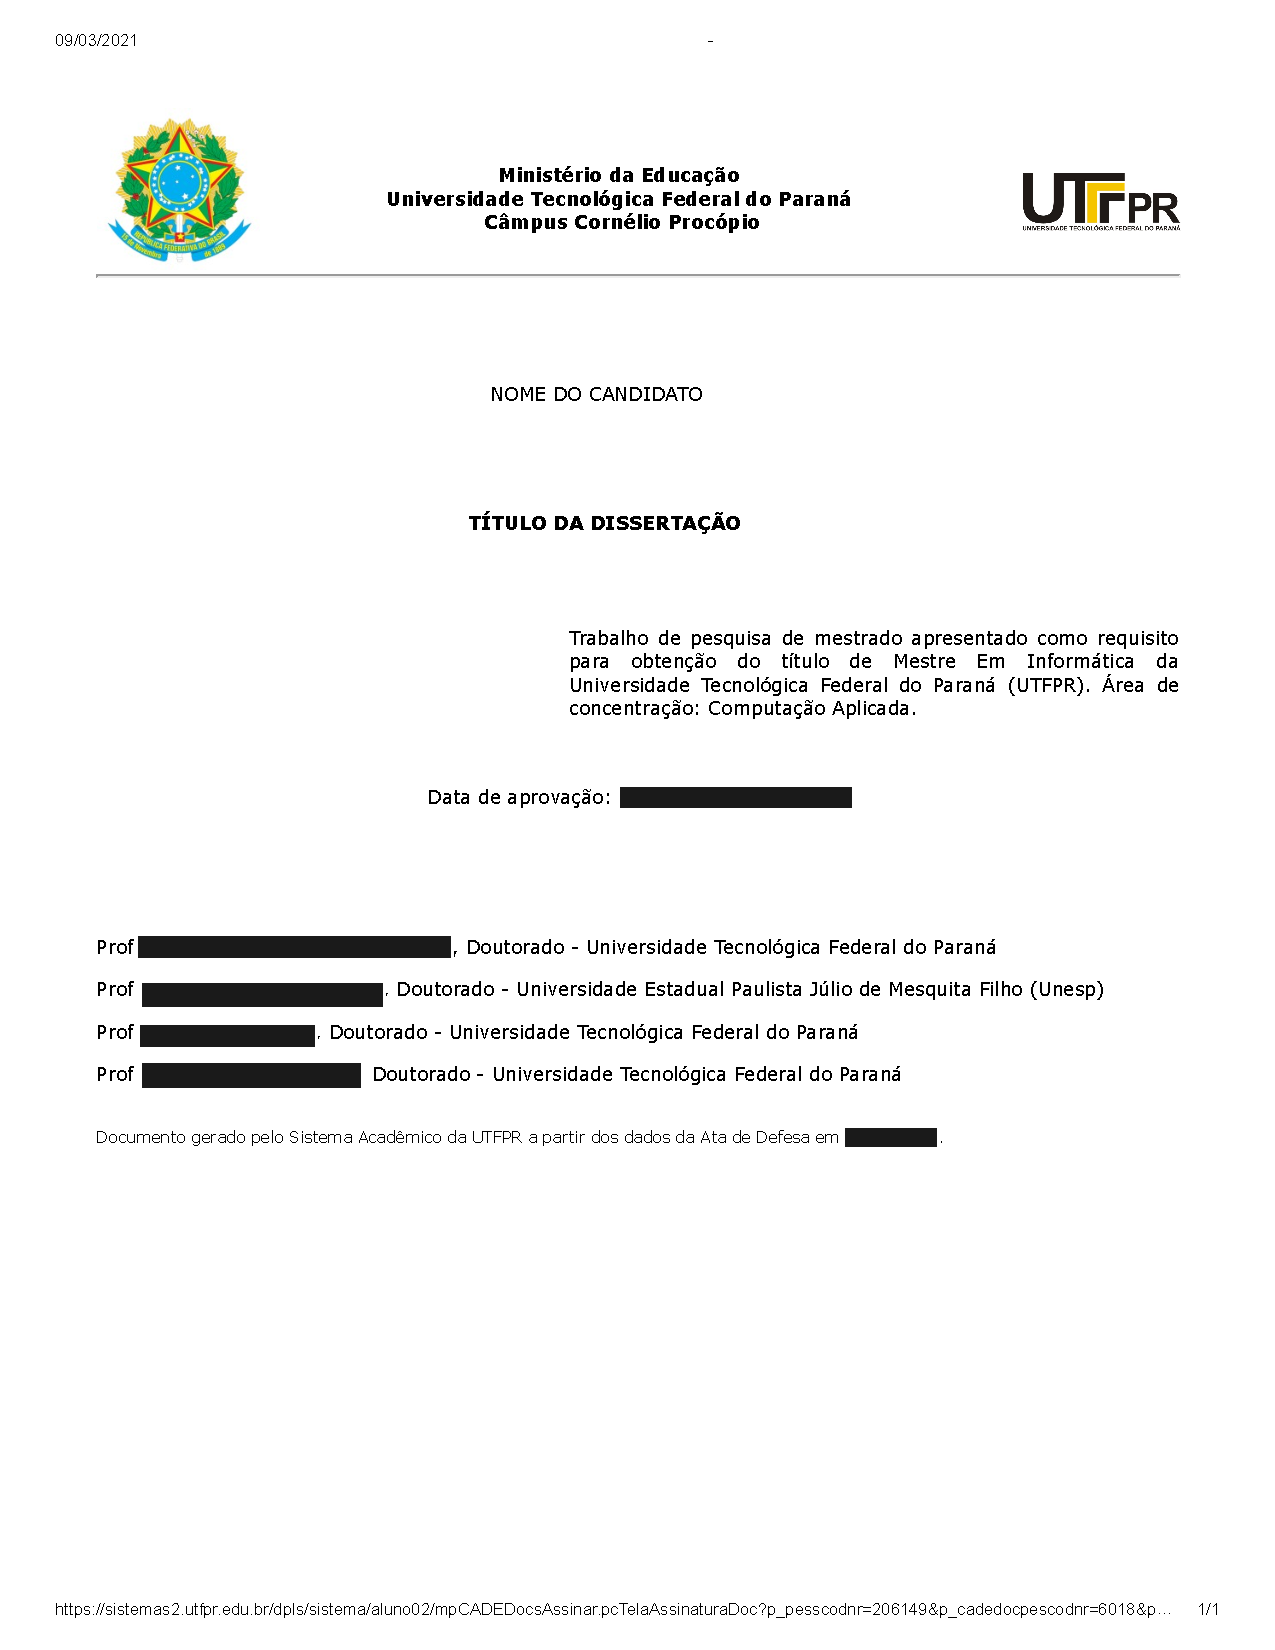
\includepdf[pages=1, pagecommand={}, trim=0 2cm 0 2cm, clip]{aprovacao.pdf}
% O comando acima inclui a folha de aprovação ocultando o cabeçalho e o rodapé gerado pelo sistema acadêmico, 
% para inserir o documento com essas informações, use "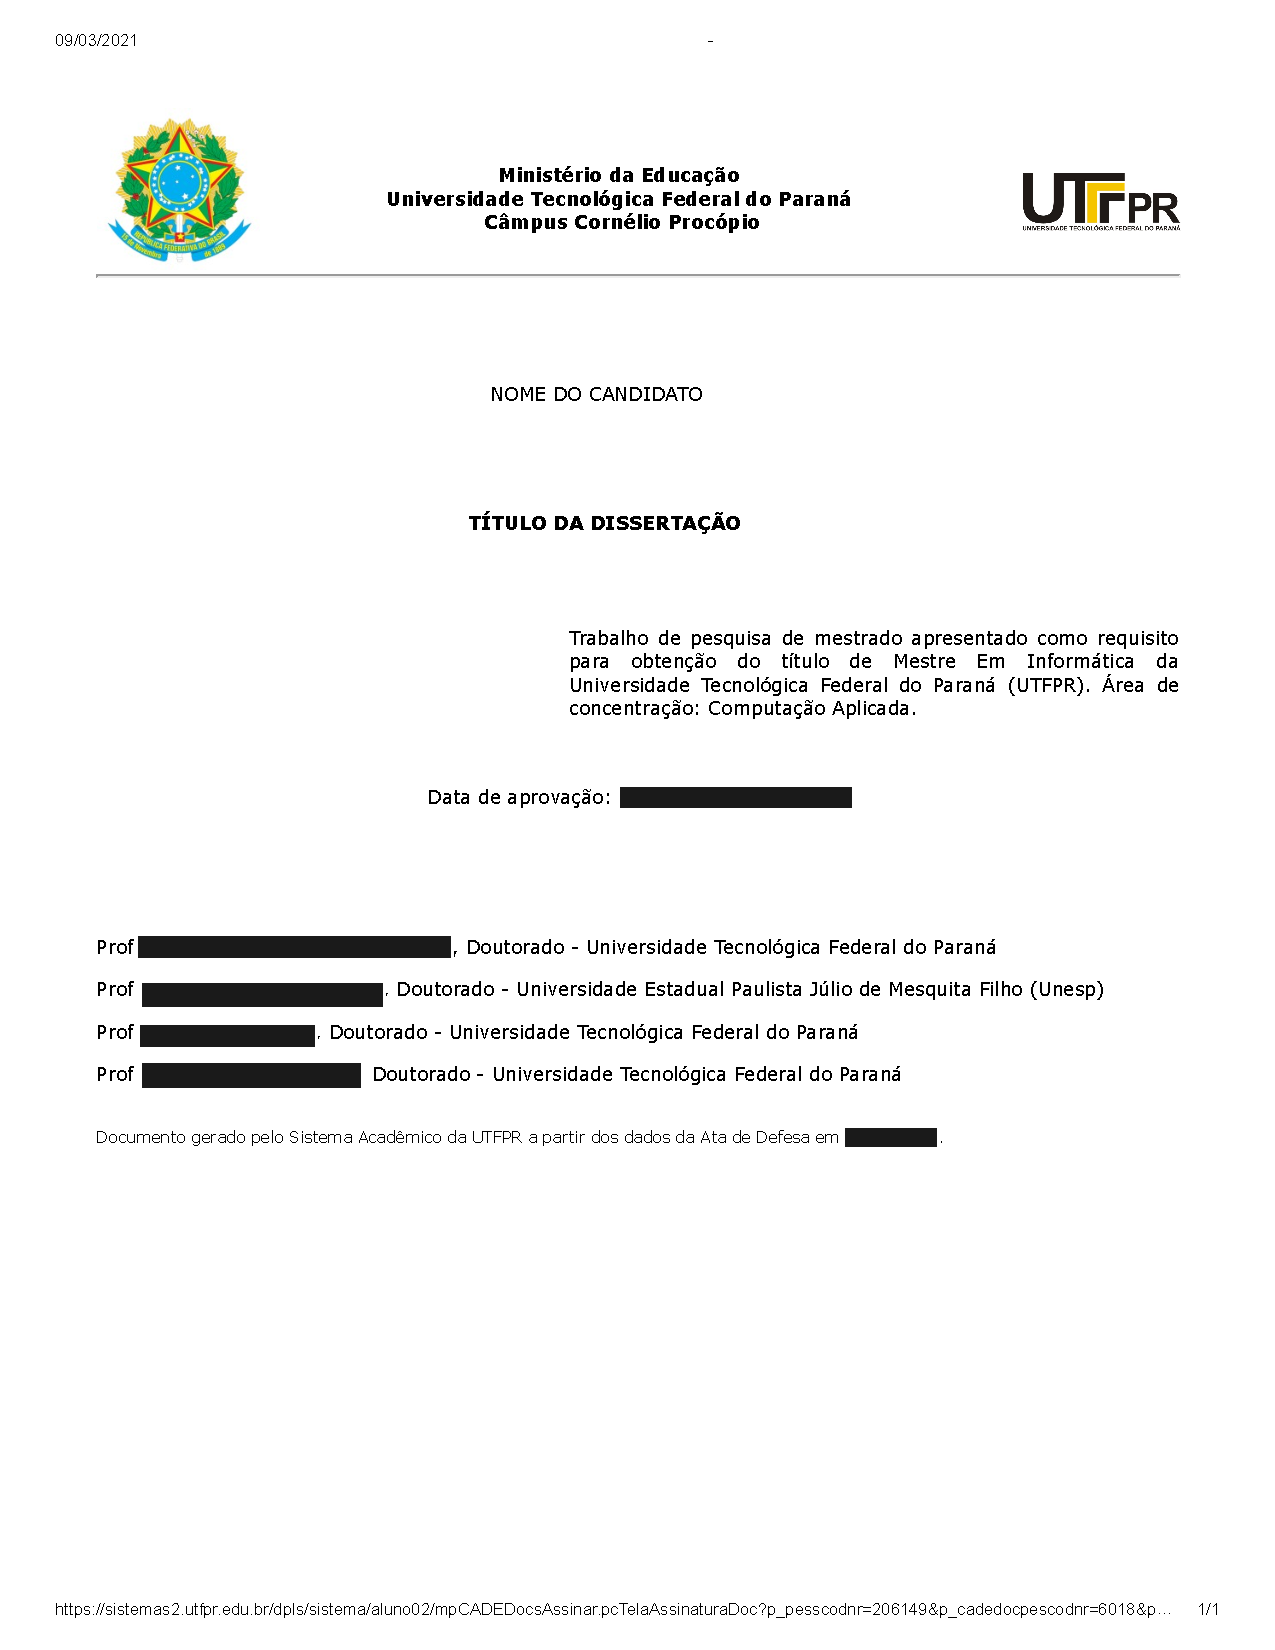
\includepdf{aprovacao.pdf}"

%%%%%%%%%%%%%%%  para usuários latex: converter o pdf em eps utilizando ferramentas como o GIMP ou inkskape
%\newpage
%\pagestyle{empty}
%\thispagestyle{empty}
%\tikz[remember picture,overlay]
%\node[opacity=1,inner sep=0pt] at (current page.center)
%{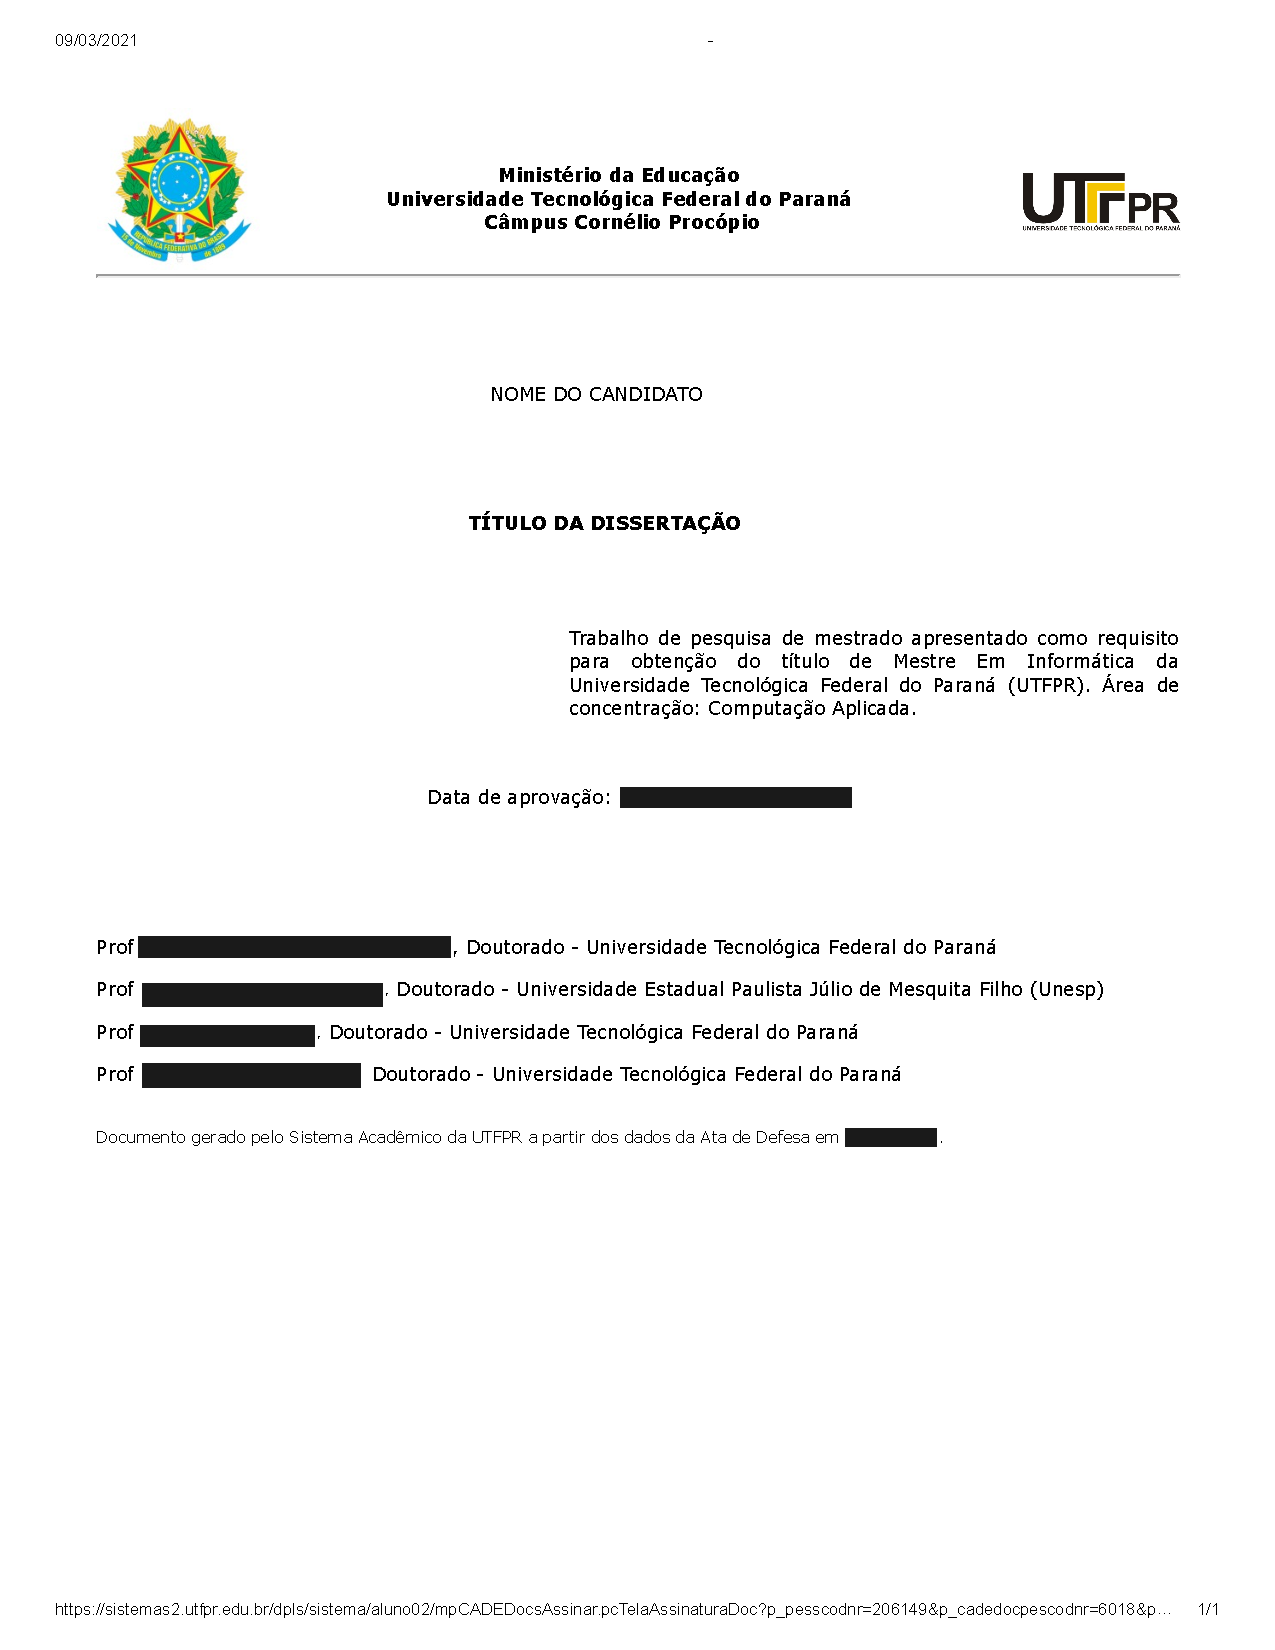
\includegraphics[width=\paperwidth,height=\paperheight]{aprovacao}};
%\cleardoublepage


% dedicatoria
\begin{dedicatoria}
À minha família, por nutrir a curiosidade que me trouxe da Física à Inteligência Artificial. Ao meu orientador e colegas, pelas conversas que transformaram ideias em código. E aos profissionais da indústria, cuja rotina inspira este esforço por processos mais sustentáveis.
\end{dedicatoria}

% agradecimentos
\begin{agradecimentos}
Ao Prof.\ Dr.\ Silvio Ricardo Rodrigues Sanches, pela orientação dedicada, pelas revisões detalhadas e pela confiança depositada nesta pesquisa interdisciplinar.

Aos membros da banca examinadora, pelas contribuições que enriqueceram a versão final deste trabalho.

À Universidade Tecnológica Federal do Paraná (UTFPR), câmpus Cornélio Procópio, e ao Programa de Pós-Graduação em Informática (PPGI), pela infraestrutura e pelo ambiente acadêmico propício à pesquisa.

À minha família, pelo apoio incondicional durante toda a trajetória do mestrado.

O presente trabalho foi realizado sem financiamento externo. Todas as ferramentas computacionais utilizadas são de código aberto ou de acesso gratuito para fins acadêmicos.
\end{agradecimentos}

% epigrafe (opcional)
% \begin{epigrafe}
% Texto da ep\'igrafe.
% \end{epigrafe}

%resumo
\begin{resumo}
Esta dissertação investiga se a incorporação de conhecimento físico-químico na engenharia de atributos --- em vez de restringi-lo às funções de perda ou às arquiteturas de rede --- melhora a predição de parâmetros de fim de corrida em Fornos Básicos a Oxigênio (BOF). Oito atributos físico-derivados, calculados a partir de balanços estequiométricos e termodinâmicos, são integrados como features de entrada a onze algoritmos de regressão supervisionada (Ridge, Lasso, ElasticNet, RF, GBM, XGBoost, LightGBM, CatBoost, SVR, KNN, MLP). Um protocolo experimental em três configurações --- A (atributos brutos), B (MLP profundo) e C (atributos brutos + físico-derivados) --- isola o efeito da engenharia de atributos do efeito de capacidade arquitetural, sobre 10.000 corridas sintéticas validadas por consistência entálpica. Os resultados demonstram que os atributos físico-derivados produzem ganhos estatisticamente significativos (Wilcoxon, $p < 0{,}05$) para o teor de carbono final (10/11 modelos melhoram; melhor MAE = 0{,}0086\,\%, CatBoost) e para o teor de fósforo final (8/11 modelos melhoram; melhor MAE = 0{,}0029\,\%, CatBoost, com seis modelos atendendo ao limiar industrial contra apenas um na linha de base), mas não resolvem o gargalo estrutural da temperatura final, limitada por variância irredutível de grandezas estocásticas não observáveis. A análise SHAP é consistente com --- sem provar --- a coerência física dos modelos: \texttt{o2\_efficiency} é o atributo de maior importância para carbono e \texttt{slag\_basicity} para fósforo, com quatro das cinco hipóteses de coerência física pré-registradas não falsificadas. A hipótese central é parcialmente confirmada: a engenharia de atributos físico-derivados melhora a predição nos alvos com relação física direta com as features propostas, mas o benefício depende do alvo e da família de modelo utilizada.
\end{resumo}

%abstract
\begin{abstract}
This dissertation investigates whether embedding physico-chemical knowledge into feature engineering --- rather than constraining loss functions or network architectures --- improves endpoint prediction in Basic Oxygen Furnace (BOF) steelmaking. Eight physics-derived features, computed from stoichiometric and thermodynamic balances, are integrated as input features into eleven supervised regression algorithms (Ridge, Lasso, ElasticNet, RF, GBM, XGBoost, LightGBM, CatBoost, SVR, KNN, MLP). A three-configuration experimental protocol --- A~(raw features), B~(deep MLP), and C~(raw + physics-derived features) --- isolates the effect of feature engineering from architectural capacity, evaluated on 10,000 synthetic heats validated by enthalpy balance consistency. Results show that physics-derived features yield statistically significant improvements (Wilcoxon, $p < 0.05$) for final carbon content (10/11 models improve; best MAE~=~0.0086\%, CatBoost) and final phosphorus content (8/11 models improve; best MAE~=~0.0029\%, CatBoost, with six models meeting the industrial threshold against only one in the baseline), but do not resolve the structural bottleneck of final temperature prediction, which is limited by irreducible variance from unobservable stochastic process variables. SHAP analysis is consistent with --- though does not prove --- physical coherence: \texttt{o2\_efficiency} is the top feature for carbon and \texttt{slag\_basicity} for phosphorus, with four of five pre-registered physical-coherence hypotheses not falsified. The central hypothesis is partially confirmed: physics-derived feature engineering improves prediction for targets with direct physical relationships to the proposed features, but the benefit depends on target variable and model family.
\end{abstract}

% listas (opcionais, mas recomenda-se a partir de 5 elementos)
\listadefiguras % geracao automatica da lista de figuras
\listadetabelas % geracao automatica da lista de tabelas
%\listadequadros % nenhum quadro definido nesta dissertação
\listadesiglas % geracao automatica da lista de siglas
\listadesimbolos % geracao automatica da lista de simbolos

% sumario
\sumario % geracao automatica do sumario


%---------- Inicio do Texto ----------
% recomenda-se a escrita de cada capitulo em um arquivo texto separado (exemplo: intro.tex, fund.tex, exper.tex, concl.tex, etc.) e a posterior inclusao dos mesmos no mestre do documento utilizando o comando \input{}, da seguinte forma:
%\input{intro.tex}
%\input{fund.tex}
%\input{exper.tex}
%\input{concl.tex}

\setstretch{1.5}
\setcounter{page}{12}


\chapter{Introdução}
\label{chp:capitulo1}

Este trabalho apresenta um arcabouço reprodutível que utiliza modelagem físico-química para aprimorar as previsões de aprendizado de máquina em contextos industriais, investigando se atributos derivados de balanços físicos — em vez de restrições na função de perda — melhoram a predição de parâmetros de fim de corrida em Fornos Básicos a Oxigênio (BOF). A metodologia se configura como um passo rumo a sistemas de IA mais interpretáveis e fisicamente coerentes para o setor de manufatura, condicionado às limitações discutidas no Capítulo~\ref{chp:con}.

%-- PROBLEMATIZAÇÃO	 --%
\section{Contexto Histórico}
\label{sec:contexto-historico}

Manufatura e analítica de dados coevoluíram ao longo de quatro revoluções industriais — da mecanização a vapor que impulsionou a produção em massa no final do século XVIII, passando pelas linhas de montagem eletrificadas do início do século XX \cite{lasi2014industry} e pela automação assistida por computador da Indústria 3.0 \cite{hermann2016industrie4}, até a integração atual de IoT, análises avançadas e IA em operações auto-otimizáveis \cite{schwab2017fourth,lu2017industry}. O aprendizado de máquina acompanhou essa trajetória: algoritmos interpretáveis (regressão linear, árvores de decisão) lançaram as bases da modelagem preditiva \cite{kuhn2013applied}, sucedidos por perceptrons multicamada e redes profundas especializadas em visão e sequências \cite{jordan2015ml}.

A fronteira mais recente incorpora leis físicas ao aprendizado por dois caminhos distintos: as Redes Neurais Informadas por Física (PINNs), que embutem restrições físicas diretamente na função de perda \cite{raissi2019pinns,cuomo2022physics}, e a síntese de atributos específicos de domínio, que insere grandezas físicas como variáveis de entrada sem alterar o objetivo de treinamento \cite{willard2020integrating,brunton2020machine}. Este trabalho segue o segundo caminho — uma distinção que orienta toda a proposta metodológica dos capítulos seguintes.

%-- MOTIVAÇÃO --%
\section{Problemas e premissas}
\label{sub:prob}

Modelos de aprendizado de máquina puramente orientados a dados atingem desempenho competitivo em muitas tarefas de regressão industrial, mas frequentemente falham ao extrapolar para regiões operacionais fora da distribuição de treino --- um problema recorrente em processos siderúrgicos com dados escassos e ruidosos\,\cite{bae2020bof,willard2020integrating}. O paradigma de Aprendizado de Máquina Informado por Física (PIML) propõe integrar conhecimento de domínio às estruturas de ML para mitigar essa limitação\,\cite{raissi2019pinns,karniadakis2021physics,cuomo2022physics}. Três topologias de integração são reconhecidas na literatura: serial (modelo físico + corretor ML), paralela (fusão de saídas) e informada por atributos (grandezas físicas como features de entrada)\,\cite{willard2020integrating,chattopadhyay2022hybrid}. As três topologias já foram aplicadas a BOF individualmente\,\cite{xia2024dmpinn,chattopadhyay2022hybrid,shao2024hybrid,bae2020bof}, mas nenhum trabalho isola sistematicamente, sob um protocolo controlado, o efeito da topologia informada por atributos frente à mesma capacidade arquitetural sem esses atributos --- a lacuna real detalhada no Capítulo~\ref{chp:capitulo3}, não a novidade da topologia em si.

No contexto específico de Fornos Básicos a Oxigênio (BOF), a predição acurada dos parâmetros de fim de corrida --- temperatura final ($T_\text{final}$), teor de carbono ($[\text{C}]_\text{final}$) e teor de fósforo ($[\text{P}]_\text{final}$) --- é determinante para a qualidade do aço --- definida neste trabalho pelas tolerâncias industriais detalhadas na Seção~\ref{sec:objetivo} --- e para a eficiência energética do processo\,\cite{bae2020bof,zhou2024bof}. O setor siderúrgico responde por aproximadamente 7--8\,\% das emissões globais de gases de efeito estufa\,\cite{worldsteel2025climate}; melhorias na predição de \textit{endpoint} podem reduzir o re-sopro e o desperdício de materiais, com impacto direto em sustentabilidade\,\cite{chattopadhyay2022hybrid}. Um estudo recente demonstra que a adição de features termodinâmicas a modelos de ML melhora a taxa de acerto em 2--4 pontos percentuais\,\cite{bae2020bof}, mas nenhum trabalho isolou sistematicamente o efeito da engenharia de atributos da capacidade arquitetural em um protocolo controlado.

Diante dessa lacuna, a \textbf{pergunta de pesquisa} desta dissertação é: \textit{a incorporação de atributos físico-derivados baseados em balanços estequiométricos e termodinâmicos como features de entrada melhora significativamente a predição de parâmetros de fim de corrida em BOF, em comparação com modelos treinados exclusivamente com variáveis brutas?}

\section{Objetivos}
\label{sec:objetivo}

O objetivo geral desta pesquisa é quantificar o ganho de precisão atribuível à engenharia de atributos baseada em balanços estequiométricos e termodinâmicos para predição de \textit{endpoint} em conversores BOF, no contexto de \textbf{regressão supervisionada} informada por física (PIML)\,\cite{willard2020integrating,cuomo2022physics}. Para tanto, propõe-se um protocolo experimental com três configurações — Config~A (atributos brutos, conjunto completo de modelos), Config~B (atributos brutos, MLP profunda com busca de arquitetura) e Config~C (atributos brutos mais os oito físico-derivados, conjunto completo de modelos) — que isola o efeito dos atributos físico-derivados (A$\times$C) do efeito da capacidade arquitetural (A$\times$B), avaliando 11 modelos de ML comuns às três configurações --- 12 na Config~C, que soma o MLP profundo exclusivo de B e C --- sobre três variáveis-alvo. Trata-se de uma \textbf{contribuição metodológica} validada sobre dados sintéticos gerados dentro de faixas físico-químicas documentadas na literatura; não constitui estudo de implantação operacional, e a validação com dados reais de planta permanece como trabalho futuro necessário\,\cite{buggineni2024synthetic}.

Os três alvos de predição são: temperatura final do banho ($T_\text{final}$), teor de carbono residual ($[\text{C}]_\text{final}$) e teor de fósforo residual ($[\text{P}]_\text{final}$). Os critérios de qualidade industrial adotados são MAE $\leq 10\,^\circ\text{C}$, MAE $\leq 0{,}020\,\%$ em massa e MAE $\leq 0{,}003\,\%$ em massa, respectivamente\,\cite{zhou2024bof,bae2020bof}. Os dados são gerados sinteticamente via Monte Carlo dentro de limites físico-químicos documentados na literatura, com plausibilidade termodinâmica validada por balanço entálpico.

\subsection{Objetivos Específicos}
\label{subsec:objetivos-especificos}

\begin{enumerate}
  \item Gerar um conjunto de dados sintético de processo BOF por amostragem de Monte Carlo dentro de faixas físico-químicas validadas pela literatura, com validação de cada instância por balanço entálpico\,\cite{buggineni2024synthetic,xia2024dmpinn};
  \item Calcular oito atributos físico-derivados — demanda teórica de O$_2$, eficiência de O$_2$, excedente entálpico, massa total oxidada, taxa de descarburação, basicidade da escória, capacidade de fusão de sucata e perda de Fe por oxidação — a partir de equações estequiométricas e termodinâmicas do processo\,\cite{chattopadhyay2022hybrid,shao2024hybrid};
  \item Treinar e otimizar o conjunto completo de modelos de regressão supervisionada — Ridge\,\cite{hoerl1970ridge}, Lasso\,\cite{tibshirani1996regression}, ElasticNet\,\cite{zou2005regularization}, Random Forest, Gradient Boosting, XGBoost, LightGBM, CatBoost\,\cite{zhou2024bof}, SVR\,\cite{widodo2007svm}, KNN\,\cite{ding2011knnimpute} e MLP\,\cite{goodfellow2016deep} — em três configurações experimentais comparáveis (A, B e C);
  \item Quantificar a diferença de desempenho (MAE, RMSE, R$^2$) entre as configurações via análise comparativa, verificando se a Config~C (físico-informada) atinge os limiares industriais de qualidade nos três alvos (MAE $\leq 10$\,°C, $\leq 0{,}020$\,\%~em~massa e $\leq 0{,}003$\,\%~em~massa, respectivamente)\,\cite{zhou2024bof,bae2020bof};
  \item Interpretar os modelos de melhor desempenho por análise SHAP\,\cite{lundberg2017unified,manojlovic2022eaf}, testando as seguintes hipóteses verificáveis de coerência física:
  \begin{description}
    \item[H1:] um atributo derivado da demanda estequiométrica de O$_2$ (\texttt{theo\_o2\_demand} ou sua forma normalizada \texttt{o2\_efficiency}) figura entre os três atributos de maior importância SHAP para $T_\text{final}$ na Config~C;
    \item[H2:] um atributo derivado da demanda estequiométrica de O$_2$ (\texttt{theo\_o2\_demand} ou \texttt{o2\_efficiency}) figura entre os três atributos de maior importância SHAP para $[\text{C}]_\text{final}$ na Config~C;
    \item[H3:] \texttt{slag\_basicity} figura entre os três atributos de maior importância SHAP para $[\text{P}]_\text{final}$ na Config~C;
    \item[H4:] o efeito marginal SHAP de \texttt{decarb\_rate} sobre $[\text{C}]_\text{final}$ é predominantemente negativo (maior taxa de descarburação prediz menor teor de carbono final);
    \item[H5:] o efeito marginal SHAP de \texttt{enthalpy\_surplus} sobre $T_\text{final}$ é predominantemente positivo (maior disponibilidade entálpica prediz maior temperatura final).
  \end{description}
  A rejeição de uma hipótese isolada é examinada quanto a explicações estruturais alternativas (por exemplo, redundância entre atributos correlatos); a rejeição da maioria das cinco, sem explicação estrutural defensável, constituiria evidência de que o modelo capturou correlações espúrias em vez de estrutura causal física.
\end{enumerate}

\section{Justificativa}
\label{sec:just}

O BOF é responsável por cerca de 70\,\% da produção mundial de aço bruto\,\cite{worldsteel2025figures}, e o setor siderúrgico como um todo responde por aproximadamente 7–8\% das emissões globais de gases de efeito estufa (Seção~\ref{sub:prob})\,\cite{worldsteel2025climate}. Melhorias na predição de \textit{endpoint} têm potencial para reduzir re-sopros e desperdício de material, com benefícios de rendimento e consumo energético a serem quantificados em trabalho futuro sobre dados reais de planta — esta dissertação estabelece a metodologia e quantifica seu ganho sobre dados sintéticos, não uma implantação operacional.

Dessa forma, as contribuições desta dissertação são três:

\begin{enumerate}
  \item \textbf{Desenho do \textit{framework}} – Uma arquitetura que sistematiza oito atributos físico-derivados do processo BOF e os combina com um conjunto de onze modelos de regressão supervisionada (doze na Config~C, incluindo o MLP profundo) otimizados via Optuna, agnóstica ao algoritmo de aprendizado;
  \item \textbf{Protocolo de avaliação controlado} – Um protocolo A$\times$B$\times$C que isola o efeito da engenharia de atributos físicos do efeito da capacidade arquitetural, sobre um conjunto de dados sintéticos gerados dentro de faixas físico-químicas documentadas na literatura e validados por consistência termodinâmica;
  \item \textbf{Evidência empírica target-dependente} – Um exame de em quais dos três alvos (T\textsubscript{final}, C\textsubscript{final}, P\textsubscript{final}) e para quais famílias de modelo a engenharia de atributos físico-derivados produz ganho estatisticamente significativo, incluindo os casos em que o ganho é nulo ou negativo\,\cite{willard2020integrating}.
\end{enumerate}

Ao quantificar onde e para quem a engenharia de atributos físicos ajuda — e onde não ajuda —, este trabalho contribui para a agenda de uma IA fisicamente fundamentada em domínios industriais, com a otimização energética/ambiental como motivação e aplicação prospectiva, não como resultado demonstrado nesta dissertação.

\section{Estrutura}
\label{sec:estrutura}

O restante do texto segue a lógica dos cinco objetivos específicos (§\,\ref{subsec:objetivos-especificos}). O Capítulo~2 estabelece a fundamentação teórica: pré-processamento e avaliação de modelos de ML, o paradigma PIML e a formulação de PINNs, a caracterização físico-química do BOF, e abordagens de geração de dados sintéticos, interpretabilidade via SHAP e arquiteturas híbridas — dando suporte conceitual a todos os cinco objetivos. O Capítulo~3, por sua vez, revisa os trabalhos relacionados em cinco eixos temáticos (fundamentos de PIML, endpoint em BOF, EAF, dados sintéticos e arquiteturas híbridas físico-informadas) e fecha com uma tabela comparativa que fundamenta o posicionamento desta contribuição frente à literatura.

Os Capítulos~4 e~5 entregam os cinco objetivos diretamente. O Capítulo~4 detalha o protocolo de geração sintética por Monte Carlo, as equações dos oito atributos físico-derivados, a defesa contra circularidade e as três configurações experimentais com o protocolo de \textit{tuning} via Optuna (Objetivos~1--4; Figura~\ref{fig:piml-pipeline}). O Capítulo~5 verifica a hipótese central por análise comparativa entre configurações e testes de Wilcoxon, avalia a robustez em extrapolação e discute a coerência física das importâncias SHAP frente às hipóteses H1--H5 (Objetivo~5), confrontando os resultados com magnitudes da literatura.

Por fim, o Capítulo~6 sintetiza o trabalho e suas contribuições, identifica as limitações inerentes ao uso de dados sintéticos e propõe direcionamentos para validação com dados reais de planta industrial.
\chapter{Fundamentação Teórica}
\label{chp:ass}

Este capítulo estabelece a base conceitual para a proposta metodológica do Capítulo~\ref{chp:capitulo4}: parte das etapas de pré-processamento e avaliação de modelos de aprendizado de máquina (Seção~\ref{sec:treinamento-ml}), avança para o paradigma de aprendizado de máquina informado por física e a formulação de PINNs (Seção~\ref{sec:des2}), caracteriza fisico-quimicamente o processo BOF (Seção~\ref{sec:des3}), e encerra discutindo geração de dados sintéticos, interpretabilidade via SHAP e arquiteturas híbridas físico-informadas (Seções~\ref{sec:dados-sinteticos-fund}--\ref{sec:arquiteturas-hibridas}).

\section{Treinamento de Modelos de Aprendizado de Máquina}
\label{sec:treinamento-ml}

Esta seção aborda as etapas preparatórias intrínsecas a treinamentos eficazes
de modelos de aprendizado de máquina. Inicia com a exploração das práticas de
limpeza de dados como base para a confiabilidade\cite{rahm2000data,kuhn2013applied,aggarwal2015outlier},
depois revisa estratégias de transformação — como escalonamento, codificação e
ajustes de lei de potência — cujos efeitos na convergência do modelo estão bem
documentados em guias aplicados de modelagem preditiva\cite{kuhn2013applied}.
Técnicas de redução de dimensionalidade, notadamente PCA e suas extensões não
lineares, são apresentadas como ferramentas comprovadas para mitigar problemas de
dimensionalidade enquanto preservam a interpretabilidade física dos fluxos de
sensores\cite{jolliffe2016pca,vandermaaten2008tsne}. Por fim, discutimos métodos
de balanceamento de conjuntos de dados que enfrentam o desbalanceamento de classes
típico de bases de falhas industriais, baseando-se em trabalhos seminais sobre SMOTE (\textit{Synthetic Minority Over-sampling Technique}) e em soluções recentes baseadas em ensembles\cite{chawla2002smote,he2009imbalanced,galar2012review}.
Em conjunto, essas referências estruturam um fluxo de pré-processamento que é ao
mesmo tempo teoricamente fundamentado e adaptado à natureza ruidosa e heterogênea
dos dados industriais do mundo real.

\subsection{Técnicas de Pré-processamento}
\label{subsec:preprocessamento}

O pré-processamento de dados constitui etapa fundamental em qualquer pipeline de aprendizado de máquina, com impacto direto na qualidade e interpretabilidade das predições\,\cite{kuhn2013applied}. Em contextos industriais, sinais brutos podem conter deriva de sensores, ruído, redundância e registros ausentes, tornando indispensáveis procedimentos de limpeza, normalização e verificação de consistência\,\cite{rahm2000data,hodge2004survey}. Descrevem-se a seguir as quatro etapas canônicas de pré-processamento e sua relevância para o contexto desta dissertação.

\textbf{Limpeza de dados.} Valores faltantes podem ser imputados por média, mediana ou técnicas avançadas como KNN \textit{imputation}, que preservam melhor as relações entre variáveis em processos contínuos\,\cite{kuhn2013applied,ding2011knnimpute}. Outliers são tratados por recorte, \textit{capping} ou transformações robustas\,\cite{aggarwal2015outlier,hodge2004survey}.

\textbf{Transformação de dados.} Normalização e padronização tornam as variáveis compatíveis com os algoritmos; em ambientes guiados por física, essas transformações devem preservar unidades e leis de conservação --- padronizações que mantenham a coerência dimensional são recomendadas\,\cite{kuhn2013applied,brunton2019ddse,willard2020integrating}.

\textbf{Redução de dimensionalidade.} Em contextos físico-informados, métodos como PCA devem ser aplicados com cautela: projeções podem descartar variáveis de baixa variância estatística, mas alta relevância metalúrgica\,\cite{jolliffe2016pca}. Nesta dissertação, os 14 atributos brutos são preservados individualmente para a análise SHAP; redução de dimensionalidade não é empregada.

\textbf{Balanceamento do conjunto de dados.} Técnicas como SMOTE endereçam desequilíbrio de classes em tarefas de classificação\,\cite{chawla2002smote,buda2018systematic}. Nesta dissertação, a tarefa é regressão supervisionada sobre dados sintéticos com distribuição aproximadamente uniforme; desequilíbrio de classe não se aplica.

\subsection{Otimização do Treinamento}
\label{subsec:otimizacao-treinamento}

Um treinamento eficaz de modelos de aprendizado de máquina depende da combinação de técnicas que aumentam o desempenho, melhoram a capacidade de generalização e otimizam a convergência\,\cite{goodfellow2016deep}.

\textbf{Engenharia e seleção de atributos.}
A criação ou transformação de atributos busca capturar melhor os padrões subjacentes aos dados. Expansões polinomiais, termos de interação e transformações guiadas por domínio enriquecem o conjunto de variáveis\,\cite{kuhn2013applied}. Já a seleção de atributos visa reduzir ruído e complexidade, aumentando a interpretabilidade; técnicas como Eliminação Recursiva de Atributos (RFE)\,\cite{guyon2002gene}, informação mútua e pontuações de importância em árvores são amplamente utilizadas nesse contexto.

\textbf{Regularização.}
A regularização previne \textit{overfitting} ao penalizar modelos excessivamente complexos. A regularização L1 (Lasso)\,\cite{tibshirani1996regression} incentiva esparsidade e faz seleção implícita de atributos; a L2 (Ridge)\,\cite{hoerl1970ridge} distribui os pesos de modo mais uniforme, gerando modelos mais suaves. O ElasticNet combina ambas, equilibrando esparsidade e estabilidade em espaços de alta dimensão onde features são correlacionadas\,\cite{zou2005regularization}.

\textbf{Otimizadores e agendamento de taxa de aprendizado.}
Otimizadores minimizam a função de perda durante o treinamento. O Gradiente Descendente Estocástico (SGD) é o método fundamental\,\cite{bottou2012sgd}, mas variantes com taxas adaptativas — RMSprop\,\cite{tieleman2012lecture} e Adam\,\cite{kingma2015adam} — alcançam convergência mais rápida e estável; Adam combina momento e escalonamento adaptativo de gradientes, tornando-se padrão em \textit{deep learning}. Estratégias de agendamento como \textit{cosine annealing} com \emph{warm restarts} (SGDR)\,\cite{loshchilov2017sgdr} e taxas cíclicas\,\cite{smith2017cyclical} oferecem flexibilidade adicional, especialmente em regimes de baixa densidade de dados.

\textbf{AutoML e seleção automatizada de modelos.} Sistemas de Aprendizado de Máquina Automatizado (AutoML) buscam automatizar o ciclo de seleção de algoritmos, engenharia de atributos e otimização de hiperparâmetros\,\cite{he2021automl}. Ferramentas como Auto-sklearn, FLAML e PyCaret implementam essa automação com diferentes filosofias: Auto-sklearn utiliza meta-aprendizado e otimização bayesiana sobre um portfólio de algoritmos scikit-learn; FLAML prioriza baixo custo computacional via busca adaptativa; PyCaret oferece uma API unificada de alto nível que encapsula todo o ciclo de modelagem — pré-processamento, comparação de modelos, tuning e avaliação — com integração nativa ao scikit-learn\,\cite{he2021automl}. Nesta dissertação, a seleção e tuning de hiperparâmetros são realizados diretamente com Optuna\,\cite{akiba2019optuna} sobre um conjunto pré-definido de onze modelos, abordagem que oferece controle total sobre o espaço de busca e reprodutibilidade integral dos experimentos em detrimento da automatização completa do portfólio.

\subsection{Avaliação dos Resultados}
\label{subsec:avaliacao}

A avaliação de modelos de aprendizado de máquina é crucial para determinar sua eficácia, capacidade de generalização e confiabilidade em aplicações reais. Em regressão — tarefa central desta dissertação —, utilizam-se o Erro Quadrático Médio (MSE), o Erro Absoluto Médio (MAE) e o coeficiente de determinação $R^{2}$\,\cite{bishop2006prml}. O MAE é particularmente relevante por sua interpretabilidade direta em unidades físicas (graus Celsius para temperatura, fração mássica para carbono e fósforo), permitindo confrontar os resultados com tolerâncias industriais estabelecidas.

\textbf{Divisão de dados e validação cruzada.}
Garantir avaliações confiáveis requer particionar o conjunto de dados em treino, validação e teste. Para conjuntos de tamanho moderado — como o dataset sintético de 10.000 corridas utilizado nesta dissertação —, a validação cruzada em $k$-partições minimiza a dependência de um único \textit{split} e fornece estimativas mais robustas de desempenho fora da amostra\,\cite{kohavi1995study}. \citeauthor{demsar2006statistical} recomenda o teste de Wilcoxon com postos assinados como alternativa não-paramétrica robusta para comparar o desempenho pareado de dois algoritmos, originalmente no contexto de acurácia de classificadores\,\cite{demsar2006statistical}; esta dissertação estende a mesma lógica pareada e não-paramétrica aos erros absolutos por instância em regressão --- uma extensão direta, já que o teste opera sobre qualquer par de amostras emparelhadas, não especificamente sobre taxas de acerto de classificação. O teste de McNemar, por contraste, exige rótulos categóricos e não se aplica a erros contínuos de regressão.

\textbf{Ferramentas de visualização.}
Para tarefas de regressão, gráficos de resíduos, dispersões entre valores previstos e observados, e métricas de influência como a distância de Cook ajudam a detectar colinearidade, heterocedasticidade e pontos influentes\,\cite{cook1977detection,belsley1980regression,anscombe1973graphs}. Tais ferramentas não apenas complementam os indicadores quantitativos, mas também permitem identificar se o modelo sistematicamente erra em determinadas regiões do espaço operacional — informação valiosa para o refinamento do conjunto de atributos físico-derivados\,\cite{inglis2022visualisation}.

\textbf{\textit{Overfitting} e \textit{underfitting}.}
\emph{Overfitting} se manifesta quando o modelo aprende ruído do conjunto de treino e falha em generalizar; disparidades acentuadas entre erros de treino e validação sinalizam esse problema\,\cite{goodfellow2016deep}. Estratégias como regularização L1/L2, \textit{dropout}\,\cite{srivastava2014dropout} e parada precoce reduzem o sobreajuste. O \emph{underfitting}, por outro lado, decorre de modelos pouco expressivos para capturar a não-linearidade do processo; nesse caso, aumentar a capacidade do modelo ou adicionar atributos físico-derivados informativos são medidas eficazes\,\cite{goodfellow2016deep}.

Ao combinar métricas rigorosas, validação cruzada e diagnósticos visuais, este trabalho adota um protocolo de avaliação único e comparável entre as três configurações experimentais para os três alvos de predição (Capítulo~\ref{chp:capitulo4}).

\section{Física e Aprendizado de Máquina}
\label{sec:des2}

Esta seção examina a convergência entre aprendizado de máquina e ciências físicas, iniciando pelas Redes Neurais Informadas por Física (PINNs) e avançando para a integração mais ampla do conhecimento físico-químico na engenharia de atributos. Destaca-se a importância de incorporar leis de domínio para aumentar a interpretabilidade e a robustez, especialmente em contextos industriais como a siderurgia.

A integração da física nos processos de treinamento de modelos de aprendizado de máquina emergiu como uma abordagem transformadora, sobretudo em domínios que exigem alta precisão, interpretabilidade e robustez \cite{cuomo2022physics,karniadakis2021physics}. Modelos puramente orientados a dados requerem, em geral, grandes volumes de amostras rotuladas; métodos informados por física, por sua vez, incorporam leis fundamentais ao processo de aprendizagem, reduzindo a dependência de dados e melhorando a capacidade de generalização \cite{raissi2019pinns,cuomo2022physics}.

As Redes Neurais Informadas por Física (PINNs) exemplificam esse paradigma ao embutir leis físicas — expressas como Equações Diferenciais Parciais (EDPs) — diretamente na função de perda da rede. Esse mecanismo penaliza desvios das restrições físicas subjacentes durante o treinamento — uma regularização suave, não uma garantia —, o que tende a produzir previsões mais fidedignas e robustas \cite{willard2020integrating,wang2021deep}. Além das PINNs, restrições baseadas em física podem ser adicionadas a diversos arcabouços de aprendizado, incluindo métodos de \textit{kernel}, modelos probabilísticos e aprendizado por reforço \cite{brunton2020machine}. Abordagens de identificação esparsa, como o SINDy (\textit{Sparse Identification of Nonlinear Dynamics}), permitem ainda descobrir equações governantes diretamente a partir de dados, complementando a família de métodos físico-informados\,\cite{brunton2016sindy}.

\subsection{Redes Neurais Informadas por Física (PINNs)}
\label{subsec:pinns}

PINNs foram concebidas para incorporar leis físicas conhecidas em modelos de \textit{deep learning} por meio da inclusão das EDPs governantes na função de perda. Dessa forma, a rede é treinada para produzir soluções que se aproximem das restrições físicas, reduzindo a necessidade de grandes conjuntos de dados rotulados em áreas onde a coleta de dados é dispendiosa, como dinâmica dos fluidos e mecânica quântica \cite{raissi2019pinns}. Ao aprender representações fundamentadas nas leis naturais, essas redes tendem a generalizar melhor para cenários não vistos, quando comparadas a modelos puramente empíricos.

\textbf{Importante para esta dissertação:} a estratégia adotada aqui \emph{não} é a das PINNs. Nenhuma restrição física é inserida na função de perda dos modelos treinados nesta pesquisa — as grandezas físico-derivadas entram exclusivamente como \emph{atributos de entrada} adicionais (engenharia de atributos), deixando a arquitetura e o objetivo de treinamento de cada modelo de regressão supervisionada inalterados (ver Capítulo~\ref{chp:capitulo4}). A discussão de PINNs nesta seção situa o trabalho na literatura de PIML mais ampla, não descreve o método proposto.

PINNs já obtiveram êxito em vários domínios, incluindo dinâmica dos fluidos computacional, análise estrutural, transferência de calor, geofísica e física médica \cite{cuomo2022physics,toscano2024pikan,cai2021heat,haghighat2020solid}. Nos estudos de aerodinâmica, por exemplo, resolvem as equações de Navier-Stokes; em ciência dos materiais, predizem relações tensão-deformação; e, em modelagem do subsolo, geram insights valiosos para exploração de petróleo e previsão de sismos \cite{toscano2024pikan,jin2021nsfnets}. Entre os desafios atuais estão a complexidade computacional (devido à necessidade de resolver EDPs durante a otimização), a sensibilidade a hiperparâmetros que equilibram perdas físicas e empíricas, e a crescente demanda por abordagens híbridas que combinem PINNs com regressão simbólica ou outras técnicas de IA para aumentar a eficiência \cite{cuomo2022physics,toscano2024pikan,wang2021deep}.

\subsection{Modelos Físico-Químicos no Aprendizado de Máquina}
\label{subsec:modelos-fisicoquimicos}

Para além do \textit{deep learning}, princípios de física e química podem guiar modelos tradicionais de aprendizado de máquina via engenharia avançada de atributos. Em aplicações industriais e científicas, os dados brutos muitas vezes carecem de estrutura suficiente para um aprendizado eficaz. A modelagem físico-química preenche essa lacuna ao gerar atributos informativos que incorporam velocidades de reação e propriedades termodinâmicas, melhorando a precisão preditiva em domínios de engenharia governados por leis de conservação, como mecânica dos fluidos e processos industriais\,\cite{brunton2020machine,willard2020integrating}.

Um estudo notável é a modelagem do balanço energético de Fornos Elétricos a Arco (EAF) integrando equações de conservação de energia como estrutura de modelos de ML. \citeauthor{logar2022eaf} integraram equações de conservação de energia ao framework de aprendizado para estimar perdas térmicas e identificar oportunidades de melhoria operacional, obtendo resultados superiores aos de modelos puramente orientados a dados\,\cite{logar2022eaf}. Complementarmente, \citeauthor{manojlovic2022eaf} aplicaram XGBoost com análise SHAP a dados de um EAF industrial para identificar os principais determinantes do consumo energético, como uso de oxigênio e peso de corrida\,\cite{manojlovic2022eaf}.

Outro exemplo de abordagem guiada por física é a modelagem de processos em Forno Básico a Oxigênio (BOF). Aqui, simulam-se reações físico-químicas chave — como oxidação de carbono e fósforo —, dinâmicas de balanço de energia e estimativa da temperatura final após o sopro de oxigênio. Cálculos estequiométricos e de entalpia oferecem atributos essenciais que aprimoram a capacidade preditiva de modelos de aprendizado de máquina \cite{xia2024dmpinn,bae2020bof,chattopadhyay2022hybrid}. A integração do perfil de fluxo de oxigênio, das massas molares e da composição da carga metálica permite capturar dinâmicas reacionais intrincadas, possibilitando previsões mais precisas sobre a composição do aço e o rendimento do processo.

Além da modelagem preditiva, modelos de ML aplicados a parâmetros operacionais do BOF --- vazão de oxigênio, padrões de sopro, composição de carga --- têm o potencial de apoiar decisões operacionais que reduzam re-sopro e desperdício de material, contribuindo para a agenda mais ampla de aplicações de aprendizado de máquina à mitigação de mudanças climáticas em processos industriais\,\cite{rolnick2019climate}; esta dissertação não testa otimização operacional diretamente, apenas a predição de \textit{endpoint} que a viabilizaria. Essa capacidade é crucial em ambientes industriais que demandam controle preciso de refino, com impacto direto na sustentabilidade.

Em síntese, incorporar leis físico-químicas aos fluxos de trabalho de aprendizado de máquina gera modelos não apenas mais precisos e generalizáveis, mas também mais transparentes e fisicamente coerentes\,\cite{raissi2019pinns,cuomo2022physics}. Das PINNs --- que incluem restrições físicas diretamente na função de perda --- até a engenharia de atributos orientada por domínio, essa integração permite que sistemas industriais operem com maior robustez e interpretabilidade, estabelecendo os alicerces para a proposta metodológica descrita no Capítulo~\ref{chp:capitulo4}.

\section{Fornos Básicos a Oxigênio (BOF): Visão Geral do Processo}
\label{sec:des3}

Os Fornos Básicos a Oxigênio (BOFs) formam a espinha dorsal da rota integrada de produção de aço, refinando o ferro-gusa líquido em aço por meio de sopro de oxigênio de alta pureza (\(\ge\!99{,}5\%\)). Na Figura~\ref{fig:bof}, o jato supersônico incide sobre o banho, promovendo oxidação preferencial de carbono, silício, manganês e fósforo, liberando calor que funde sucata e mantém o metal próximo de \(1650^{\circ}\text{C}\). A cinética heterogênea dessas reações e seu balanço termodinâmico estão bem estabelecidos\cite{bae2020bof}. O processo é não linear e multiescala --- envolve turbulência, transporte de massa entre banho e escória e projeção de gotículas ---, o que o torna ideal para modelos híbridos que unem balanços estequiométricos e aprendizado de máquina\cite{bae2020bof,xia2024dmpinn}.

\textbf{Materiais de entrada.}
A carga metálica de um BOF inclui ferro-gusa líquido a 1250–1450\,°C — com composição típica de 3,8–4,8\,\% C; 0,3–1,2\,\% Si; 0,2–0,8\,\% Mn; 0,06–0,15\,\% P —, sucata interna ou comercial (10–30\,\% da carga total) para controle térmico, e eventuais pré-reduzidos (DRI/HBI). Estas são as mesmas faixas operacionais adotadas na amostragem sintética do Capítulo~\ref{chp:capitulo4} (Tabela~\ref{tbl:ranges-sinteticos}). Os fundentes — cal calcítica e dolomita — ajustam a basicidade da escória ($\text{CaO}/\text{SiO}_2\approx3$) e favorecem a remoção de P e S\,\cite{madhavan2020heatbalance}. O oxigênio soprado pelo topo é complementado por argônio ou nitrogênio insuflados pelo fundo para homogeneizar o banho metálico ao longo do sopro.

\begin{figure}[H]
\centering
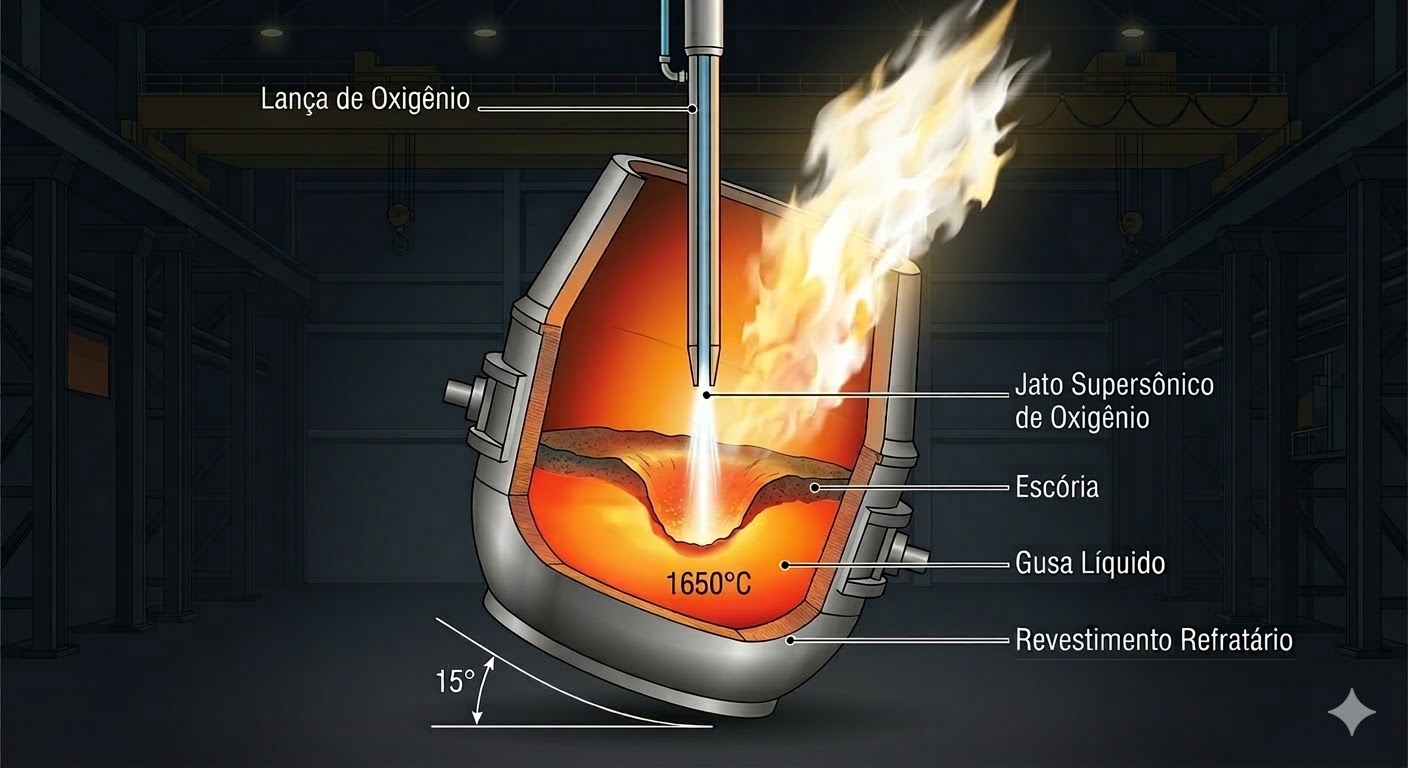
\includegraphics[width=0.55\textwidth]{Images/BOF_Illustration}
\caption{Seção transversal de um BOF (Forno a Oxigênio Básico). Lança de O\textsubscript{2}, escória, gusa líquido e revestimento refratário. (Nano Banana Pro~3.)}
\label{fig:bof}
\end{figure}

\textbf{Variáveis monitoradas e alvos de qualidade.}
O acerto simultâneo da temperatura final ($T_\text{final}=1650\pm10$\,°C) e do teor de carbono residual ($0{,}03$–$0{,}08$\,\%) é crítico: esses dois parâmetros definem a eficiência de dessulfuração subsequente e a estabilidade do vazamento contínuo\,\cite{wang2020endpoint,diaz2019hotmetaltemp}. Modelos de ML com atributos tabulares amplos aplicados a dados reais de planta já reportam MAE de temperatura da ordem de $8\,^\circ\text{C}$ e de carbono da ordem de $7\times10^{-3}\,\%$~em~massa\,\cite{zhou2024bof} --- valores mais rigorosos do que os limiares de $10\,^\circ\text{C}$ e $0{,}020\,\%$ adotados nesta dissertação (Seção~\ref{sec:objetivo}); a diferença reflete o uso de dados reais de planta e de um conjunto de atributos tabulares mais amplo do que o desta dissertação, não uma meta menos ambiciosa (Seção~\ref{sec:comparacao-literatura}, Capítulo~\ref{chp:resultados}). Além de C, Si e Mn, monitoram-se P, S, Cr, Ni e Cu, bem como Fe e O dissolvidos; o potencial redox de cada espécie compete pelo oxigênio disponível, e conhecer essas interações é essencial para dosar fluxantes e otimizar o perfil de sopro\,\cite{bae2020bof}.

\textbf{Balanços estequiométrico e entálpico.}
Antes do sopro, balanços de massa determinam a quantidade de sucata, cal e oxigênio necessária para as reações principais:
\[
\text{C + O}_2 \rightarrow \text{CO}_x,\quad
\text{Si + O}_2 \rightarrow \text{SiO}_2,\quad
\text{Mn + O}_2 \rightarrow \text{MnO},
\]
enquanto um balanço de entalpia calcula que aproximadamente 65\,\% do calor total provém do calor sensível do gusa e 35\,\% do ganho exotérmico das oxidações\,\cite{madhavan2020heatbalance}. Esses cálculos definem a janela de sucata que pode ser fundida sem comprometer a temperatura alvo e a fração ótima de fluxantes. A explicitação desses balanços como atributos de entrada de modelos de ML — em vez de deixá-los implícitos nos dados brutos — é o princípio central da engenharia de atributos físico-derivados adotada nesta dissertação.

\textbf{Integração sensor–modelo.}
A Figura~\ref{fig:bof-process-flow} sintetiza as sete etapas operacionais do sopro, do carregamento do metal líquido à escorificação final. Sinais brutos de termopares, medidores de vazão e espectrômetros são filtrados e temporalmente alinhados para gerar variáveis derivadas — massa oxidada, excedente de entalpia, eficiência de uso de O\textsubscript{2} — que condensam relações não-lineares de difícil aprendizado direto\,\cite{willard2020integrating}, conforme ilustrado na Figura~\ref{fig:bof-process-diagram}. Tais atributos alimentam modelos híbridos que refinam a estimativa do \emph{endpoint} em tempo quase real\,\cite{chattopadhyay2022hybrid,xia2024dmpinn}, reduzindo a necessidade de amostragens manuais e melhorando a robustez operacional em condições de carga variável.

\begin{figure}[htbp]
\centering
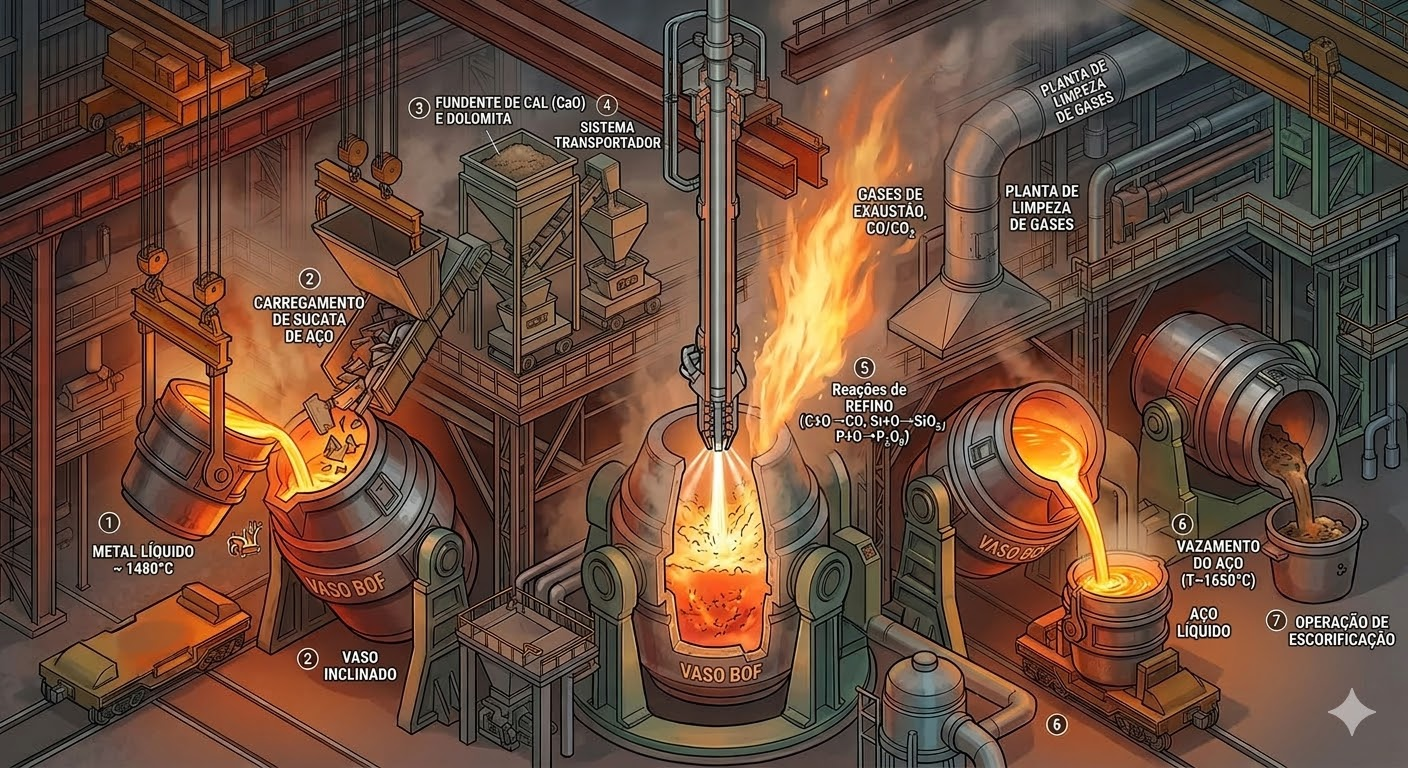
\includegraphics[width=0.82\textwidth]{Images/FLuxo_BOF}
\caption{Fluxo operacional completo do processo BOF: (1)~carregamento do metal líquido ($\approx\!1480$\,°C), (2)~inclinação do vaso, (3)~adição de fundentes (CaO, dolomita) via sistema transportador, (4)~sopro de O\textsubscript{2} com reações de refino, (5)~exaustão e limpeza de gases CO/CO\textsubscript{2}, (6)~vazamento do aço líquido e (7)~escorificação. Ilustração gerada com auxílio de inteligência artificial (Nano Banana Pro~3).}
\label{fig:bof-process-flow}
\end{figure}

\begin{figure}[htbp]
\centering
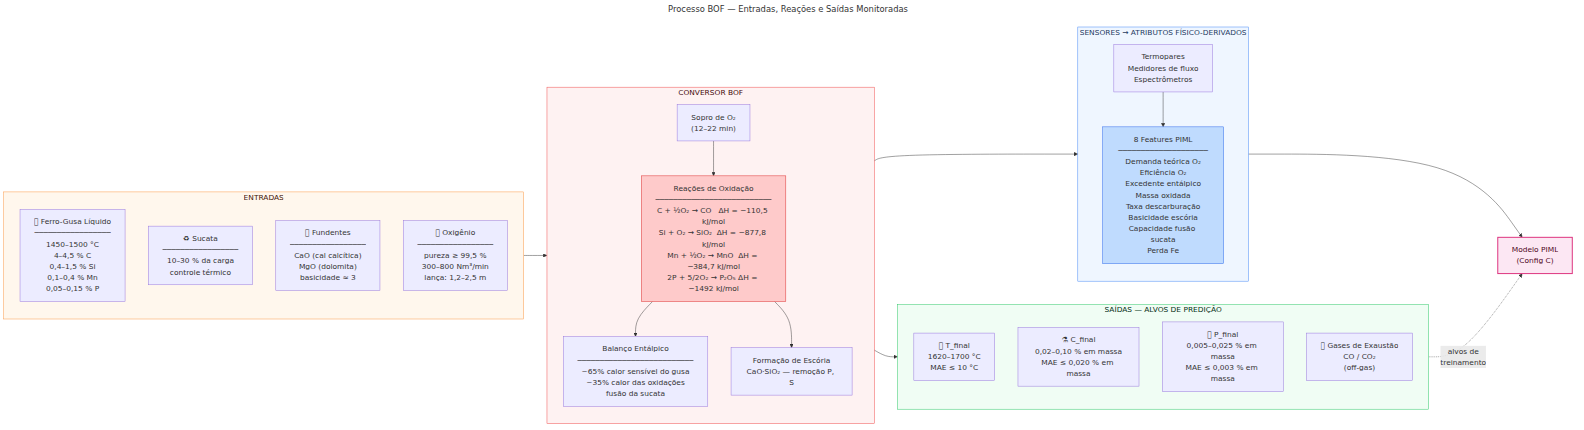
\includegraphics[width=0.82\textwidth]{Images/diagrams/05_bof_process}
\caption{Diagrama esquemático do processo BOF: entradas (gusa líquido, sucata, fundentes e O\textsubscript{2}), reações de oxidação no conversor, saídas monitoradas (T\textsubscript{final}, C\textsubscript{final}, P\textsubscript{final}) e derivação dos oito atributos físico-derivados a partir dos sinais de sensores para o modelo PIML.}
\label{fig:bof-process-diagram}
\end{figure}

Em conclusão, tem-se que compreender a natureza, estequiometria e entalpia dos insumos --- gusa, sucata, fluxantes e oxigênio --- é decisivo para atingir temperatura e composição alvo na primeira tentativa. A hipótese central desta dissertação (Seção~\ref{sec:objetivo}) é que a inclusão explícita desses balanços nos atributos do modelo melhora o erro preditivo além de fornecer explicações físico-químicas potencialmente mais transparentes; o Capítulo~\ref{chp:resultados} avalia essa hipótese empiricamente, com resultado dependente do alvo de predição.

%-------------------------------------------------------------------%
\section{Geração de Dados Sintéticos para Processos Industriais}
\label{sec:dados-sinteticos-fund}

Dados rotulados de processos industriais são escassos por razões práticas: cada corrida em um BOF ou ciclo de um EAF representa custo elevado de energia e materiais, e a coleta de rótulos precisos (composição química final, temperatura) exige análise laboratorial ou sensores especializados\,\cite{buggineni2024synthetic}. Essa escassez motiva o uso de dados sintéticos gerados por modelos físico-matemáticos como substitutos para o treinamento de modelos de ML.

A literatura sobre dados sintéticos tabulares distingue quatro categorias de métodos de geração: amostragem paramétrica (Monte Carlo e variantes), modelos baseados em cópulas, redes generativas adversariais (GANs) e autoencoders variacionais (VAEs)\,\cite{buggineni2024synthetic,melo2024synthetic}. Para processos industriais cujas restrições físicas são bem conhecidas e o tamanho amostral alvo é da ordem de milhares — não milhões —, a amostragem Monte Carlo com validação por balanço de massa ou energia é mais transparente, reproducível e computacionalmente econômica do que abordagens generativas profundas\,\cite{buggineni2024synthetic,morales2025synthetic}.

A validade dos dados sintéticos depende de dois requisitos: (i) as faixas de amostragem devem cobrir o espaço operacional real do processo, derivadas de fontes industriais ou literatura especializada; e (ii) cada instância gerada deve satisfazer as leis de conservação pertinentes, descartando-se amostras fisicamente implausíveis\,\cite{buggineni2024synthetic,melo2024synthetic}. \citeauthor{melo2024synthetic} demonstraram que dados sintéticos gerados sob essas condições produzem modelos de ML com desempenho comparável aos treinados em dados reais para tarefas de regressão de processo em gêmeos digitais industriais\,\cite{melo2024synthetic}. \citeauthor{morales2025synthetic} confirmaram resultado análogo para manutenção preditiva, concluindo que dados sintéticos fisicamente coerentes permitem generalização adequada desde que as distribuições marginais e as correlações relevantes do processo sejam preservadas\,\cite{morales2025synthetic}.

Uma limitação inerente à abordagem sintética é que os modelos treinados aprendem a estrutura imposta pelo gerador, não necessariamente a do processo real. Portanto, métricas de desempenho obtidas em dados sintéticos devem ser interpretadas como evidências de viabilidade metodológica, não como estimativas de performance em planta\,\cite{giannini2022synthetic}. A validação em dados reais é etapa obrigatória antes de qualquer implantação industrial.

%-------------------------------------------------------------------%
\section{Interpretabilidade em Modelos de ML Industrial}
\label{sec:interpretabilidade}

Modelos de aprendizado de máquina de alta capacidade — como Random Forest, XGBoost e redes neurais profundas — atingem baixo erro preditivo em muitos problemas industriais, mas permanecem como caixas-pretas do ponto de vista do operador de processo\,\cite{inglis2022visualisation}. A interpretabilidade é essencial nesse contexto por duas razões: (i) permite validar se o modelo capturou relações fisicamente coerentes, e não correlações espúrias presentes nos dados de treinamento; e (ii) aumenta a confiança e a aceitação pelos profissionais que devem tomar decisões com base nas predições\,\cite{inglis2022visualisation,manojlovic2022eaf}.

Entre os métodos de interpretabilidade disponíveis, destacam-se três abordagens principais: importância por permutação, \textit{Integrated Gradients} e SHAP. A importância por permutação mede o aumento do erro ao embaralhar aleatoriamente os valores de um atributo, sendo simples e agnóstica ao modelo, porém sensível a correlações entre atributos e incapaz de fornecer explicações por instância\,\cite{inglis2022visualisation}. \textit{Integrated Gradients} oferece explicações locais baseadas em gradientes, sendo restrito a modelos diferenciáveis e, portanto, inaplicável a modelos de árvore\,\cite{inglis2022visualisation}. O método SHAP (\textit{SHapley Additive exPlanations}), fundamentado na teoria de jogos cooperativos, atribui a cada atributo uma contribuição marginal para a predição de cada instância\,\cite{lundberg2017unified}. Ao contrário de medidas de importância globais (como a impureza média em Random Forests), SHAP fornece explicações locais — por instância — e é consistente: se um atributo se torna mais importante, seu valor SHAP aumenta. Para esta dissertação, SHAP é a escolha natural por três razões: (i) é agnóstico ao algoritmo, aplicando-se igualmente a modelos lineares, Random Forest, XGBoost e MLP; (ii) fornece explicações locais com garantias axiomáticas de consistência e eficiência; e (iii) possui implementações eficientes (\texttt{TreeExplainer}) que tornam sua aplicação computacionalmente viável para os modelos de ensemble avaliados. \citeauthor{manojlovic2022eaf} aplicaram SHAP a modelos de eficiência energética em EAF e demonstraram que os atributos com maior importância SHAP correspondiam às variáveis operacionais que especialistas de processo já identificavam como determinantes — uso de oxigênio e peso de corrida —, validando a coerência física do modelo\,\cite{manojlovic2022eaf}.

Para o contexto desta dissertação, a análise SHAP serve como mecanismo de validação físico-informada: espera-se que atributos derivados de balanços de massa e energia (\texttt{theo\_o2\_demand}, \texttt{enthalpy\_surplus}, \texttt{slag\_basicity}) apresentem alta importância nos modelos treinados com a configuração físico-informada (Config~C), e que as direções de influência correspondam ao comportamento esperado pela termodinâmica\,\cite{manojlovic2022eaf,xia2024dmpinn}. Por exemplo, \texttt{slag\_basicity} deve influenciar positivamente a remoção de fósforo: maior basicidade favorece a oxidação de P para a escória\,\cite{bae2020bof}.

%-------------------------------------------------------------------%
\section{Arquiteturas Híbridas Físico-Informadas}
\label{sec:arquiteturas-hibridas}

A literatura identifica três topologias principais para integrar modelos físicos e de ML em sistemas híbridos, ilustradas na Figura~\ref{fig:hybrid-architectures}\,\cite{chattopadhyay2022hybrid,willard2020integrating}. Na arquitetura \textbf{serial}, modelo físico e modelo de ML trocam informação em múltiplas etapas de um mesmo pipeline, com a saída de um alimentando a entrada do outro; \citeauthor{chattopadhyay2022hybrid} adotam essa topologia em BOF, com modelos termodinâmicos de balanço de entalpia e oxigênio fornecendo estimativas iniciais e redes neurais treinadas nas variáveis brutas realimentando suas predições de volta aos modelos teóricos (Capítulo~\ref{chp:capitulo3})\,\cite{chattopadhyay2022hybrid}. Na arquitetura \textbf{paralela}, as saídas do modelo físico e do modelo de ML são combinadas por uma camada de fusão que aprende pesos adaptativos; \citeauthor{shao2024hybrid} utilizam estrutura análoga para predição do tempo de sopro\,\cite{shao2024hybrid}.

A terceira topologia — \textbf{informada por atributos} — não exige que o componente físico seja diferenciável nem que faça parte do grafo computacional do modelo de ML. Em vez disso, grandezas calculadas por modelos físicos (balanços de massa, energia, estequiometria) são incorporadas como variáveis de entrada adicionais\,\cite{willard2020integrating}. Essa abordagem é compatível com qualquer algoritmo de ML e impõe o menor custo de implementação, sendo vantajosa quando o componente físico não precisa ser diferenciável e quando a integração deve ser feita de forma agnóstica ao algoritmo de aprendizado\,\cite{willard2020integrating}.

O \textit{framework} físico-informado de \citeauthor{wang2025phoenix} para soldagem robótica, publicado na \textit{Nature Communications}, demonstra a escalabilidade da abordagem informada por atributos para processos de manufatura de alta complexidade, obtendo ganhos expressivos em relação a linhas de base puramente orientadas a dados e a modelos físicos puros\,\cite{wang2025phoenix}. Esses resultados reforçam a escolha metodológica desta dissertação: a Config~C implementa a topologia informada por atributos, calculando os oito atributos físico-derivados definidos na Seção~\ref{subsec:feature-engineering} e incorporando-os ao conjunto de features de todos os modelos avaliados.

\begin{figure}[htbp]
\centering
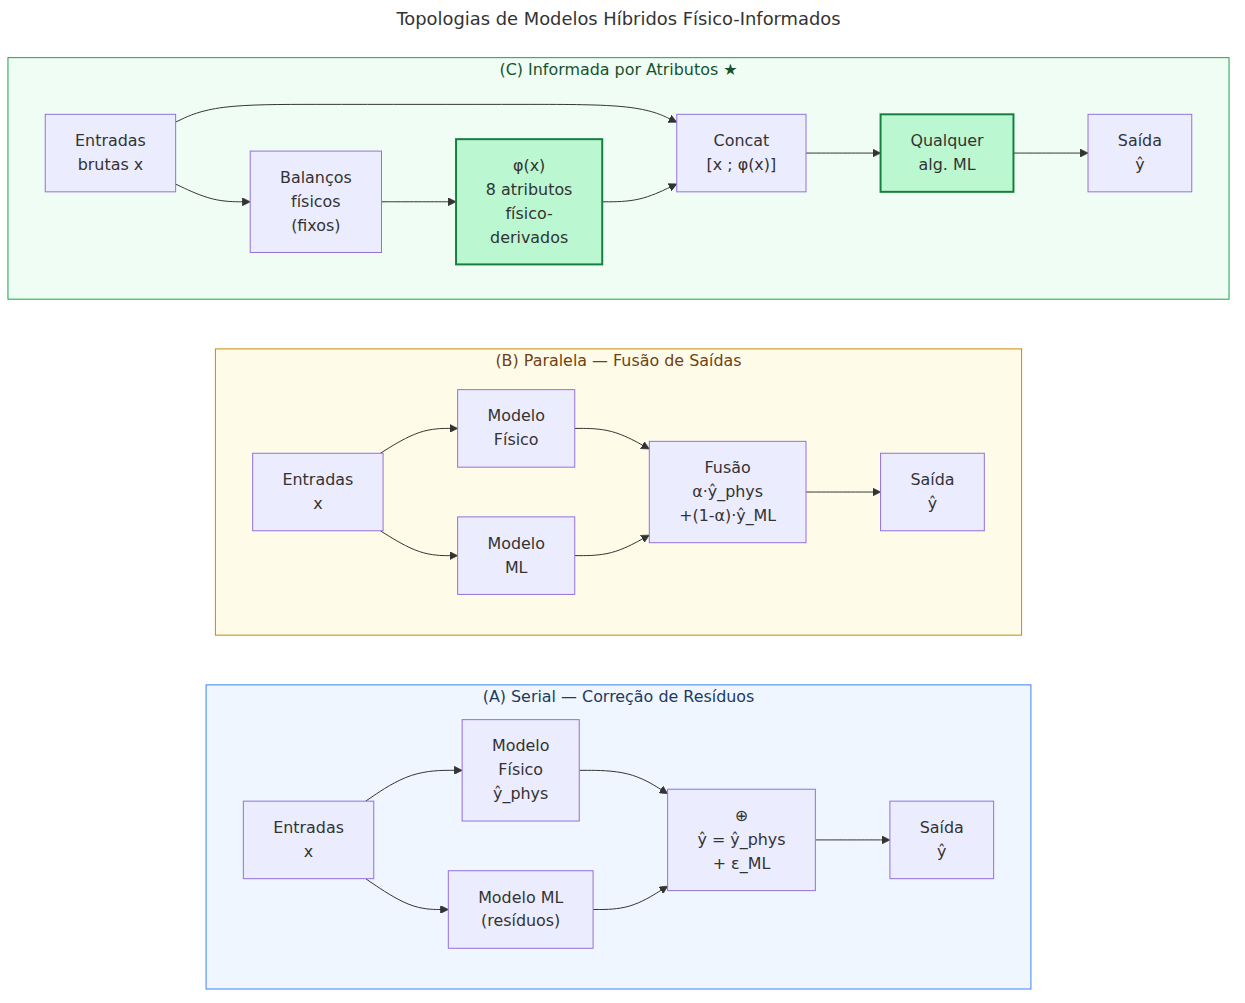
\includegraphics[width=0.78\textwidth,height=0.28\textheight,keepaspectratio]{Images/diagrams/03_hybrid_architectures}
\caption{Topologias de modelos híbridos físico-informados: (A)~serial com correção de resíduos, (B)~paralela com camada de fusão e (C)~informada por atributos — arquitetura adotada nesta dissertação. Adaptado de \,\cite{willard2020integrating}.}
\label{fig:hybrid-architectures}
\end{figure}
\chapter{Trabalhos Relacionados}
\label{chp:capitulo3}

Este capítulo revisa a literatura diretamente relacionada à predição de endpoint em processos siderúrgicos via aprendizado de máquina informado por física. A organização segue uma progressão do geral ao específico: parte dos fundamentos de PIML, avança para aplicações em fornos BOF e EAF, examina abordagens de geração de dados sintéticos industriais e, por fim, discute arquiteturas híbridas físico-informadas. A análise encerra com uma tabela comparativa e a identificação das lacunas que motivam a proposta desta dissertação.

%-------------------------------------------------------------------%
\section{Fundamentos de PIML Aplicados à Siderurgia}
\label{sec:piml-fundamentos}

A abordagem de Redes Neurais Informadas por Física (PINNs) foi formalizada por \citeauthor{raissi2019pinns} ao incorporar equações diferenciais parciais diretamente na função de perda do treinamento, permitindo que a rede neural resolva problemas diretos e inversos com supervisão parcial\,\cite{raissi2019pinns}. A formulação original demonstrou que, ao penalizar violações de leis físicas durante o gradiente descendente, é possível reduzir substancialmente a quantidade de dados rotulados necessária para treinar modelos precisos em domínios governados por equações de conservação. Esse paradigma abriu caminho para aplicações em transferência de calor, escoamento de fluidos e dinâmica estrutural.

Revisões abrangentes consolidaram o campo do PIML, estabelecendo vocabulário e taxonomia comuns\,\cite{cuomo2022physics,willard2020integrating,karniadakis2021physics}. A taxonomia adotada nesta dissertação, seguindo \citeauthor{willard2020integrating}, distingue três topologias de integração entre física e ML: \textit{serial} (um modelo físico alimenta, ou é realimentado por, um modelo de ML), \textit{paralela} (física e ML operam em ramos independentes cujas saídas são combinadas, tipicamente na função de perda, como nos PINNs clássicos\,\cite{raissi2019pinns}) e \textit{informada por atributos} (grandezas físicas pré-computadas entram como variáveis de entrada de um modelo de ML padrão, sem alterar seu objetivo de treinamento)\,\cite{willard2020integrating}. Esta última é a abordagem adotada nesta dissertação, na forma de engenharia de atributos pré-computados (Config~C, Capítulo~\ref{chp:capitulo4}). As três topologias são categorias idealizadas: sistemas reais frequentemente combinam elementos de mais de uma, e a fronteira entre elas é permeável dependendo do nível de abstração adotado na análise\,\cite{cuomo2022physics}. Um resultado transversal na literatura é que restrições físicas codificadas nos modelos aumentam a capacidade de extrapolação para regiões fora do domínio de treinamento --- propriedade especialmente relevante em processos industriais onde dados experimentais são escassos e caros\,\cite{willard2020integrating}.

%-------------------------------------------------------------------%
\section{Predição de Endpoint em Fornos Básicos a Oxigênio}
\label{sec:bof-endpoint}

A predição de endpoint em conversores BOF — temperatura final do banho, teor de carbono residual e, mais recentemente, fósforo — é um problema de regressão supervisionada com alta relevância industrial, pois erros de predição implicam reprocessamento dispendioso e desperdício energético\,\cite{chattopadhyay2022hybrid,zhou2024bof}. O uso de redes neurais para esse problema não é recente: \citeauthor{cox2002neural} já aplicavam computação neural à predição de endpoint em BOF há mais de duas décadas\,\cite{cox2002neural}, com desempenho e disponibilidade de dados de planta condicionados pelo estado da arte de ML da época. A literatura mais recente revisada nesta seção converge para arquiteturas que integram algum nível de conhecimento físico-químico, seja pela seleção cuidadosa de variáveis de entrada ou pela imposição de restrições no treinamento — o foco desta dissertação --- sem que isso implique que a modelagem estatística/ANN pré-PIML tenha sido superada de forma generalizada.

\citeauthor{xia2024dmpinn} propuseram o modelo dmPINNs (\textit{data-driven and mechanism-based Physics-Informed Neural Networks}) para predição do teor de carbono final em BOF\,\cite{xia2024dmpinn}. A arquitetura é \textit{paralela}: uma sub-rede extrai parâmetros latentes ($\alpha$, $\beta$) de uma equação cinética de descarburação apresentada pelos autores, que produz uma predição mecanicista $C_\text{cal}$; uma segunda sub-rede orientada a dados produz $C_\text{pre}$; o resultado final é a média ponderada $C_\text{dmPINN} = 0{,}5 \cdot C_\text{cal} + 0{,}5 \cdot C_\text{pre}$ (notação dos autores, distinta do $[\text{C}]_\text{final}$ desta dissertação), com função de perda que penaliza ambas as branches simultaneamente. Os resultados são reportados em termos de \textit{hit rates} para limiares de $\pm 0{,}009$, $\pm 0{,}012$ e $\pm 0{,}020$\,\%~em~massa, obtendo ganho de $+5{,}23$\,pp sobre o BPNN de linha de base no limiar mais restritivo. Esta arquitetura é fundamentalmente diferente da adotada nesta dissertação: o presente trabalho insere grandezas físicas como \textit{features} de entrada do modelo, não como restrição na função de perda.

\citeauthor{zhou2024bof} realizaram uma comparação sistemática entre algoritmos de ML e aprendizado profundo para predição de endpoint no BOF, com 13.528 corridas reais da Hesteel Group\,\cite{zhou2024bof}. Entre os modelos tabulares (45 variáveis brutas de composição, adições e O$_2$), CatBoost obteve o menor MAE para P ($2{,}28 \times 10^{-3}$\,\%~em~massa) e C ($6{,}92 \times 10^{-3}$\,\%~em~massa), enquanto LightGBM foi superior para temperatura (7{,}96\,°C). Os autores também incorporaram sete curvas de off-gas como séries temporais, combinadas ao modelo tabular via um \textit{backbone} TCN+ResCNN; esse modelo combinado reduz o MAE de teste dos três alvos simultaneamente --- não apenas de temperatura --- para $2{,}15 \times 10^{-3}$\,\% (P), $6{,}41 \times 10^{-3}$\,\% (C) e $5{,}78$\,°C (T), com MAE de $2{,}39 \times 10^{-3}$\,\%, $6{,}23 \times 10^{-3}$\,\% e $7{,}68$\,°C, respectivamente, em teste de campo real --- este último consistentemente pior que o de teste \textit{offline} para os três alvos, ilustrando o custo de generalização de laboratório para planta mesmo com dados reais. Nenhuma feature físico-derivada foi utilizada, o que confirma diretamente a lacuna endereçada por esta dissertação.

O trabalho de \citeauthor{chattopadhyay2022hybrid} apresentou um método híbrido para predição de endpoint em BOF com intercâmbio de informação serial em múltiplas etapas\,\cite{chattopadhyay2022hybrid}: modelos termodinâmicos de balanço de entalpia e oxigênio (MM\_T, MM\_C, MM\_P) fornecem estimativas iniciais de T, C e P, enquanto redes neurais independentes (ANN\_T, ANN\_C, ANN\_P) são treinadas nas variáveis brutas; na etapa híbrida, as predições das ANNs são realimentadas como entradas dos modelos teóricos — por exemplo, $\hat{C}_\text{ANN}$ substitui a assunção de carbono mediano no balanço entálpico de temperatura. Essa troca bidirecional reduz o NRMSE de predição de P em 9{,}77\% e de C em 3{,}7\% frente aos modelos teóricos isolados. A topologia é classificada como \textit{serial} na taxonomia de\,\cite{willard2020integrating} e constitui referência metodológica para a configuração C desta dissertação. \citeauthor{bae2020bof} demonstraram que grupos de atributos termodinâmicos elevam em 2–4 pontos percentuais as taxas de acerto para temperatura e fósforo, evidenciando que features físico-derivadas contribuem para estabilidade preditiva sob variações operacionais\,\cite{bae2020bof}.

A literatura em predição de endpoint BOF abrange desde regressão linear regularizada até redes neurais profundas\,\cite{zhou2024bof,chattopadhyay2022hybrid}. A evidência coletada indica que nenhum modelo supera consistentemente todos os outros em todos os alvos, justificando a estratégia adotada neste trabalho de comparar um conjunto amplo e fixo de modelos (Tabela~\ref{tbl:modelos-ml}, Capítulo~\ref{chp:capitulo4}) com otimização de hiperparâmetros individual via Optuna\,\cite{akiba2019optuna}, em vez de restringir a comparação a uma única arquitetura \textit{a priori}. O modelo híbrido de \citeauthor{shao2024hybrid}, que combina um modelo de balanço de oxigênio (OBM) com uma rede neural profunda para predição do tempo de sopro, complementa essa perspectiva ao demonstrar que variáveis físico-derivadas específicas do processo elevam o desempenho preditivo\,\cite{shao2024hybrid}.

%-------------------------------------------------------------------%
\section{Modelagem de Fornos EAF e Interpretabilidade}
\label{sec:eaf-interpretabilidade}

Embora o foco desta dissertação seja o BOF, estudos em fornos a arco elétrico (EAF) oferecem contribuições metodológicas relevantes, especialmente no que tange à interpretabilidade de modelos de ML aplicados a processos siderúrgicos. \citeauthor{skrjanc2022eaf} avaliaram a importância de variáveis em modelos preditivos de EAF usando análise de importância por permutação, identificando que peso de sucata e temperatura de corrida dominam as predições de processo\,\cite{skrjanc2022eaf}. O estudo demonstra que análise de importância de atributos permite verificar a coerência física das explicações — por exemplo, confirmando que variáveis de carga metálica dominam os resultados, conforme esperado pela termodinâmica.

\citeauthor{logar2022eaf} modelaram o balanço energético de um EAF industrial para estimar perdas térmicas e identificar oportunidades de melhoria operacional, integrando equações de conservação de energia como estrutura de modelos de ML\,\cite{logar2022eaf}. Complementarmente, \citeauthor{manojlovic2022eaf} aplicaram XGBoost com análise SHAP a dados de um EAF industrial, mostrando que os atributos de maior importância SHAP (uso de oxigênio, peso de corrida) correspondiam às variáveis operacionais que especialistas de processo já identificavam como determinantes\,\cite{manojlovic2022eaf}. Esse último trabalho fundamenta diretamente o uso de SHAP como ferramenta de validação física nesta dissertação: espera-se que atributos derivados de balanços estequiométricos (como demanda teórica de O$_2$ e basicidade da escória) ocupem posições de alta importância nos modelos treinados com a configuração físico-informada.

%-------------------------------------------------------------------%
\section{Geração de Dados Sintéticos para Processos Industriais}
\label{sec:dados-sinteticos}

A escassez de dados rotulados é um obstáculo recorrente em aplicações industriais de ML, onde cada corrida representa um custo elevado e os rótulos (composição química final, temperatura) exigem medições analíticas precisas\,\cite{buggineni2024synthetic}. A geração de dados sintéticos emerge como alternativa para viabilizar o treinamento de modelos quando o volume de dados reais é insuficiente.

\citeauthor{buggineni2024synthetic} propuseram um \textit{framework} sistemático para aumentar dados de manufatura com instâncias sintéticas, validando a abordagem em múltiplos cenários industriais\,\cite{buggineni2024synthetic}. Os autores estabelecem que a validade dos dados sintéticos depende do respeito a restrições físicas do processo durante a geração — princípio central da metodologia desta dissertação, implementado via validação por balanço entálpico com tolerância de 10\%. \citeauthor{melo2024synthetic} exploraram a geração de dados sintéticos especificamente no contexto de gêmeos digitais industriais, discutindo métricas de fidelidade que garantem que os dados gerados preservem as distribuições e correlações do processo real\,\cite{melo2024synthetic}.

A escolha de Monte Carlo com validação por balanço físico como técnica de geração é fundamentada na literatura: métodos baseados em amostragem de distribuições físicas são mais adequados do que abordagens generativas (GANs, VAEs) quando o tamanho amostral alvo é pequeno e as restrições físicas são bem conhecidas\,\cite{buggineni2024synthetic,morales2025synthetic}. \citeauthor{morales2025synthetic} reforçam esse ponto em revisão focada em manutenção preditiva industrial, concluindo que dados sintéticos fisicamente coerentes permitem generalização comparável a dados reais para tarefas de regressão de processo\,\cite{morales2025synthetic}. \citeauthor{giannini2022synthetic} demonstraram a geração de datasets de manufatura via simulação de eventos discretos, mostrando que modelos físicos de baixa fidelidade são suficientes para produzir instâncias de treino úteis\,\cite{giannini2022synthetic}.

%-------------------------------------------------------------------%
\section{Posicionamento frente às Arquiteturas Híbridas}
\label{sec:hibridas}

Conforme as três topologias de integração físico-ML descritas na Seção~\ref{sec:arquiteturas-hibridas} (serial, paralela e informada por atributos), os trabalhos revisados em BOF cobrem as três: \citeauthor{chattopadhyay2022hybrid} adotam a abordagem serial\,\cite{chattopadhyay2022hybrid}, \citeauthor{xia2024dmpinn} a paralela\,\cite{xia2024dmpinn}, \citeauthor{shao2024hybrid} também a paralela, com balanço de O$_2$\,\cite{shao2024hybrid}, e \citeauthor{bae2020bof} a informada por atributos\,\cite{bae2020bof}. Esta dissertação posiciona-se na mesma terceira topologia de \citeauthor{bae2020bof} com a Config~C — a novidade não está, portanto, na topologia em si (Seção~\ref{sec:analise-lacunas} detalha a lacuna real).

%-------------------------------------------------------------------%
\section{Tabela Comparativa e Análise das Lacunas}
\label{sec:analise-lacunas}

Nenhum dos trabalhos revisados realiza simultaneamente as três operações que definem a proposta desta dissertação: (i) isolar o efeito da engenharia de atributos do efeito de capacidade arquitetural mediante um protocolo A×B×C controlado, com o mesmo conjunto de modelos e protocolo de \textit{tuning} em ambos os braços da comparação; (ii) usar SHAP não apenas como ferramenta de ranqueamento de importância, mas como mecanismo de validação de coerência física, testando hipóteses pré-registradas sobre a direção e a posição relativa dos atributos físico-derivados; e (iii) tratar temperatura, carbono e fósforo como três alvos independentes sobre o mesmo protocolo experimental. Como a Tabela~\ref{tbl:trabalhos-relacionados} deixa explícito, a topologia informada por atributos por si só \emph{não} é a lacuna — \citeauthor{bae2020bof} já a aplica a BOF nos três alvos\,\cite{bae2020bof}; a lacuna está no protocolo de avaliação controlado que isola a contribuição específica da engenharia de atributos.

\begin{table}[H]
\centering
\caption{Síntese dos principais trabalhos relacionados a PIML em processos siderúrgicos. N: tamanho amostral; Dados: reais de planta industrial (real) ou sintéticos/simulados (sint.).}
\label{tbl:trabalhos-relacionados}
\scriptsize
\resizebox{\textwidth}{!}{%
\setlength{\tabcolsep}{3pt}
\begin{tabular}{|p{2.6cm}|p{1.1cm}|p{2.3cm}|p{1.5cm}|p{1.3cm}|p{1.7cm}|p{2.3cm}|}
\hline
\textbf{Referência} & \textbf{Processo} & \textbf{Abordagem física} & \textbf{Eng.\ Atrib.} & \textbf{Alvos} & \textbf{N; Dados} & \textbf{Contribuição} \\ \hline
\citeauthor{xia2024dmpinn} (\citeyear{xia2024dmpinn})\,\cite{xia2024dmpinn} & BOF & Paralela: eq.\ cinética + rede & Nenhuma (perda) & C & N/D; real & +5,23\,pp hit rate \\ \hline
Chattopadhyay et al. (\citeyear{chattopadhyay2022hybrid})\,\cite{chattopadhyay2022hybrid} & BOF & Serial: termodin.\ + ANNs & Implícita & T, C, P & N/D; real & $-$9,77\% NRMSE P \\ \hline
\citeauthor{shao2024hybrid} (\citeyear{shao2024hybrid})\,\cite{shao2024hybrid} & BOF & Paralela: balanço O$_2$ + DNN & Balanço O$_2$ & Tempo sopro & N/D; real & Features balanço O$_2$ \\ \hline
\citeauthor{bae2020bof} (\citeyear{bae2020bof})\,\cite{bae2020bof} & BOF & 17 features termod. & Físico-deriv. & T, C, P & N/D; real & $+$2--4\,pp hit rate \\ \hline
\citeauthor{zhou2024bof} (\citeyear{zhou2024bof})\,\cite{zhou2024bof} & BOF & Off-gas temporal & Domínio & T, C & 13.528; real & Benchmark SOTA \\ \hline
\citeauthor{wang2020endpoint} (\citeyear{wang2020endpoint})\,\cite{wang2020endpoint} & BOF & \textit{Review} & --- & C & --- & Síntese de métodos de predição de C \\ \hline
\citeauthor{ghalati2023review} (\citeyear{ghalati2023review})\,\cite{ghalati2023review} & BOF & \textit{Review} & --- & T, C, P & --- & Síntese de ML aplicado a BOF \\ \hline
\citeauthor{skrjanc2022eaf} (\citeyear{skrjanc2022eaf})\,\cite{skrjanc2022eaf} & EAF & Importância variáveis & Nenhuma & Energia & N/D; real & Domin.\ peso sucata \\ \hline
\citeauthor{logar2022eaf} (\citeyear{logar2022eaf})\,\cite{logar2022eaf} & EAF & Balanço energético & Implícita & Energia & N/D; real & Híbrido físico-ML \\ \hline
\citeauthor{manojlovic2022eaf} (\citeyear{manojlovic2022eaf})\,\cite{manojlovic2022eaf} & EAF & XGBoost + SHAP & Nenhuma & Energia & N/D; real & SHAP valida coerência física (O$_2$, peso corrida) \\ \hline
\citeauthor{wang2025phoenix} (\citeyear{wang2025phoenix})\,\cite{wang2025phoenix} & Manuf. (solda) & Físico-informado & Físico-deriv. & Múltiplos & N/D; real & Escalabilidade em manufatura complexa \\ \hline
\textbf{Esta dissertação} & \textbf{BOF} & \textbf{Informada por atributos} & \textbf{Físico-deriv.\ (8)} & \textbf{T, C, P} & \textbf{10.000; sint.} & \textbf{Protocolo A$\times$B$\times$C + SHAP como validação} \\ \hline
\end{tabular}}
\end{table}

A análise da Tabela~\ref{tbl:trabalhos-relacionados} revela dois aspectos relevantes, nenhum deles sendo a topologia em si. Primeiro, a coluna N;\,Dados deixa explícito o contraste central desta dissertação frente à literatura: os trabalhos em BOF revisados usam dados reais de planta (a maioria sem reportar N publicamente), enquanto esta dissertação usa 10.000 corridas sintéticas — uma limitação de validade externa discutida no Capítulo~\ref{chp:con}, não uma vantagem metodológica. Segundo, mesmo entre os trabalhos que usam atributos físico-derivados (\citeauthor{bae2020bof}\,\cite{bae2020bof}, \citeauthor{wang2025phoenix}\,\cite{wang2025phoenix}), nenhum isola o efeito da engenharia de atributos de um efeito de capacidade arquitetural via comparação controlada com o mesmo conjunto de modelos e protocolo de \textit{tuning} em ambos os lados.

A literatura existente raramente avalia o impacto das features físico-derivadas de forma isolada, controlando outros fatores. Comparações entre conjuntos de features (brutas vs. brutas+físicas) com a mesma família de modelos e mesmo protocolo de tuning são escassas, tornando difícil atribuir ganhos de desempenho especificamente à engenharia de atributos\,\cite{zhou2024bof,chattopadhyay2022hybrid}. Esta dissertação busca preencher essa lacuna ao adotar três configurações experimentais comparáveis — Config~A (brutas, conjunto completo de modelos), Config~B (brutas, MLP profunda) e Config~C (brutas + físico-derivadas, conjunto completo) — que permitem isolar o efeito da engenharia de atributos da escolha de arquitetura. Os limiares de qualidade industrial adotados como critério de avaliação são MAE $\leq 10$\,°C para temperatura, $\leq 0{,}020$\,\%~em~massa para carbono e $\leq 0{,}003$\,\%~em~massa para fósforo\,\cite{zhou2024bof,bae2020bof} — valores inspirados nos limiares de \textit{hit rate} reportados nesses trabalhos, mas não diretamente equivalentes a eles: um \textit{hit rate} de $\pm10$\,°C descreve a fração de corridas dentro de uma janela, não um limite superior de MAE agregado, e o MAE efetivamente associado a esse \textit{hit rate} em \citeauthor{zhou2024bof} é de aproximadamente 5,78\,°C (Seção~\ref{sec:bof-endpoint}) — um critério mais rigoroso do que os 10\,°C adotados aqui.

Finalmente, embora \citeauthor{bae2020bof} e \citeauthor{zhou2024bof} já tratem o fósforo como alvo, \citeauthor{xia2024dmpinn} foca exclusivamente em carbono e \citeauthor{chattopadhyay2022hybrid} modela fósforo apenas como parte secundária do pipeline serial. Esta dissertação trata T\textsubscript{final}, C\textsubscript{final} e P\textsubscript{final} como três alvos independentes sob o mesmo protocolo controlado, avaliando se a basicidade da escória — atributo físico-derivado diretamente relacionado à eficiência de desfosforação\,\cite{bae2020bof} — aparece como feature relevante nos modelos via análise SHAP.

\chapter{Proposta}
\label{chp:capitulo4}

Este capítulo descreve a metodologia proposta para avaliar o impacto da engenharia de atributos físico-derivados na predição de endpoint em convertedores BOF. A tarefa é de \textbf{regressão supervisionada}: dados os parâmetros operacionais de entrada de uma corrida, predizer T\textsubscript{final}, C\textsubscript{final} e P\textsubscript{final} ao fim do sopro. A proposta se estrutura em quatro etapas — geração de dados, engenharia de atributos, treinamento comparativo e avaliação — executadas em três configurações experimentais distintas que permitem isolar os efeitos da escolha de arquitetura e do conjunto de features.

\begin{figure}[H]
\centering
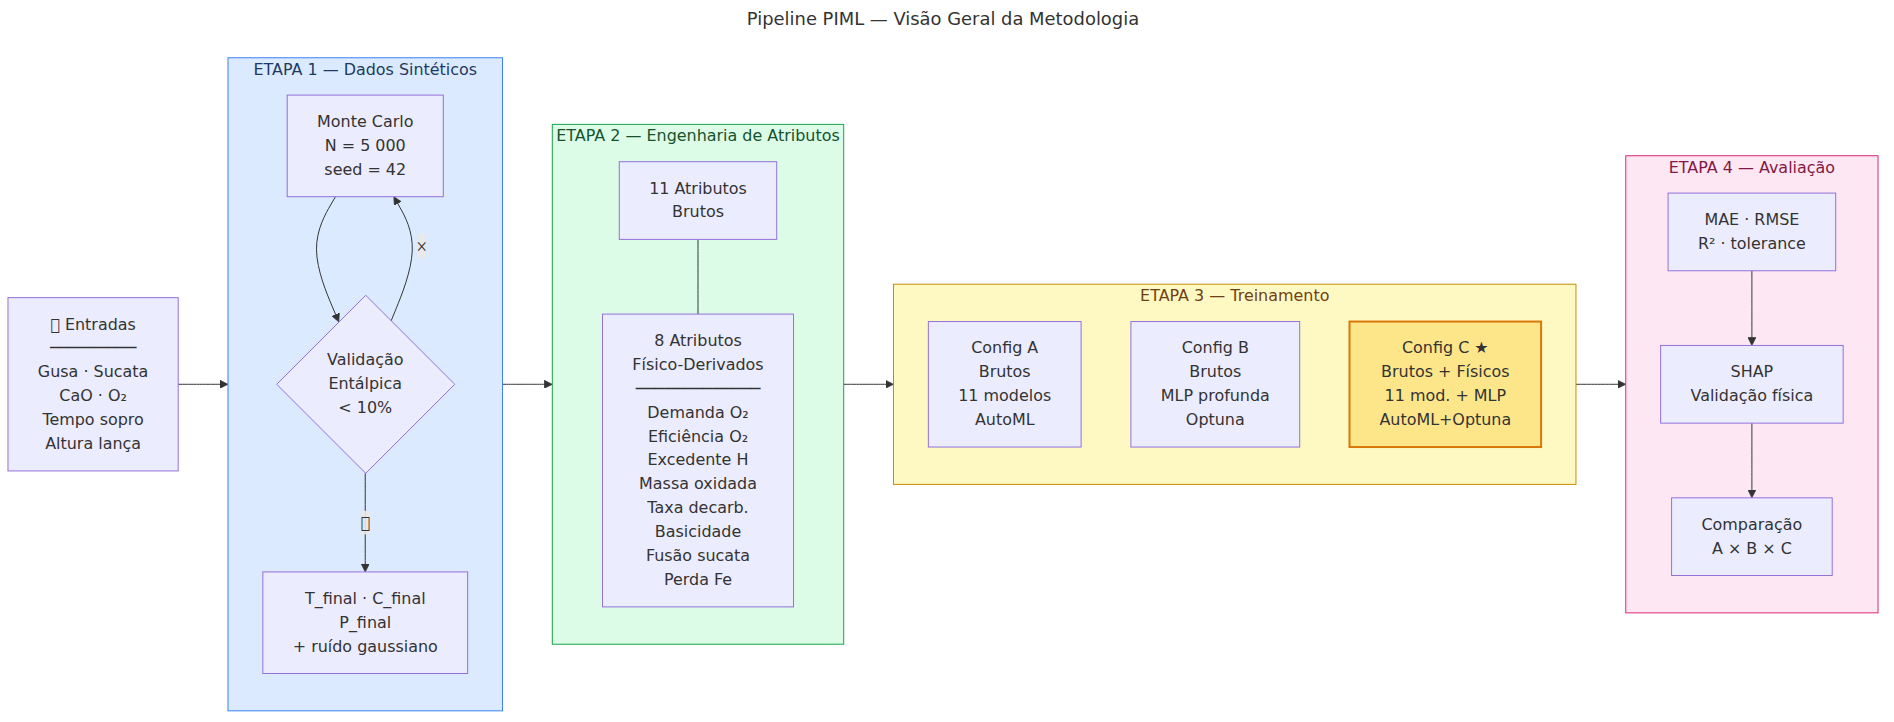
\includegraphics[width=0.88\textwidth,height=0.35\textheight,keepaspectratio]{Images/diagrams/01_piml_pipeline}
\caption{Visão geral do \textit{pipeline} metodológico proposto em quatro etapas: (1)~geração de dados sintéticos por Monte Carlo, (2)~engenharia de atributos físico-derivados, (3)~treinamento comparativo nas Configurações A, B e~C, e (4)~avaliação por métricas, análise de extrapolação e SHAP.}
\label{fig:piml-pipeline}
\end{figure}

%-------------------------------------------------------------------%
\section{Materiais}
\label{sec:materiais}

Os materiais computacionais necessários compreendem (i) o conjunto de dados sintético gerado especificamente para este trabalho, (ii) os modelos físico-químicos customizados que determinam os atributos físico-derivados e validam a plausibilidade das amostras, e (iii) as bibliotecas Python para AutoML, otimização de hiperparâmetros e interpretabilidade.

\subsection{Geração de Dados Sintéticos}
\label{subsec:dados-sinteticos}

Na ausência de dados reais de planta industrial, o conjunto de treinamento é gerado por amostragem de Monte Carlo\,\cite{buggineni2024synthetic,melo2024synthetic}. O procedimento adota $N = 10000$ amostras com semente \texttt{seed=42} para reprodutibilidade. Cada amostra é obtida por amostragem uniforme independente nas faixas físico-químicas da Tabela~\ref{tbl:ranges-sinteticos}, derivadas da literatura especializada em BOF\,\cite{xia2024dmpinn,chattopadhyay2022hybrid,bae2020bof}.

\textbf{Dados e constantes utilizados.} Nenhum dado industrial proprietário foi empregado neste trabalho. Todas as constantes físicas utilizadas --- capacidades caloríficas, entalpias de reação, razões estequiométricas e faixas operacionais --- são extraídas exclusivamente de literatura científica publicada\,\cite{cai2021heat,bae2020bof,chattopadhyay2022hybrid,xia2024dmpinn}. As referências específicas de cada constante constam nas equações da Tabela~\ref{tbl:features-fisicas} e nos comentários do código-fonte disponibilizado.

\begin{table}[H]
\centering
\caption{Faixas físico-químicas das 14 variáveis de entrada amostradas para geração de dados sintéticos. Duas delas ($S_\text{hm}$ e altura da lança) são amostradas e oferecidas como atributos aos modelos, mas não são lidas pelas equações físicas do gerador (Capítulo~\ref{chp:resultados}, Seção~\ref{sec:extrapolacao}).}
\label{tbl:ranges-sinteticos}
\small
\begin{tabular}{|p{4.2cm}|c|c|c|c|}
\hline
\textbf{Variável} & \textbf{Símbolo} & \textbf{Mín} & \textbf{Máx} & \textbf{Unidade} \\ \hline
Massa do gusa & $m_\text{hm}$ & 150 & 320 & t \\ \hline
Temperatura do gusa & $T_\text{hm}$ & 1250 & 1450 & °C \\ \hline
Carbono no gusa & $C_\text{hm}$ & 3{,}8 & 4{,}8 & \%~em~massa \\ \hline
Silício no gusa & $\text{Si}_\text{hm}$ & 0{,}3 & 1{,}2 & \%~em~massa \\ \hline
Manganês no gusa & $\text{Mn}_\text{hm}$ & 0{,}2 & 0{,}8 & \%~em~massa \\ \hline
Fósforo no gusa & $P_\text{hm}$ & 0{,}06 & 0{,}15 & \%~em~massa \\ \hline
Enxofre no gusa & $S_\text{hm}$ & 0{,}01 & 0{,}05 & \%~em~massa \\ \hline
Fração de sucata & $f_\text{scrap}$ & 0{,}10 & 0{,}30 & — \\ \hline
Carbono na sucata & $C_\text{scrap}$ & 0{,}05 & 0{,}25 & \%~em~massa \\ \hline
Adição de CaO & — & 15 & 60 & kg/t \\ \hline
Adição de MgO & — & 5 & 20 & kg/t \\ \hline
Fluxo de O$_2$ & — & 300 & 800 & Nm$^3$/min \\ \hline
Tempo de sopro & $t_\text{blow}$ & 12 & 22 & min \\ \hline
Altura da lança & — & 1{,}2 & 2{,}5 & m \\ \hline
\end{tabular}
\end{table}

Após a amostragem, cada instância é validada por dois critérios combinados por E-lógico — balanço entálpico e balanço de massa\,\cite{xia2024dmpinn,chattopadhyay2022hybrid} —, ambos exigidos para que a amostra seja aceita, embora, como discutido adiante, apenas o critério entálpico se mostre empiricamente restritivo dentro das faixas amostradas desta dissertação. O calor de entrada $Q_\text{in}$ inclui o calor sensível do gusa e o calor liberado pelas reações de oxidação dos elementos C, Si, Mn e P; o calor de saída $Q_\text{out}$ inclui o calor sensível do aço (base de massa do gusa, com a fusão da sucata contabilizada separadamente como o sorvedouro $Q_\text{scrap}$) e as perdas térmicas do processo, modeladas pela fração complementar $(1-\eta_\text{eff})$ da eficiência térmica específica da corrida (calibração e distribuição de $\eta_\text{eff}$ detalhadas na Seção~\ref{subsec:ameacas-validade}):

\begin{align}
Q_\text{in}  &= m_\text{hm}\,C_{p,\text{hm}}\,(T_\text{hm} - T_\text{ref}) + \sum_i \frac{m_\text{hm}\,x_i\,|\Delta H_i|}{M_i} \label{eq:q-in} \\
Q_\text{out} &= m_{\text{steel},\text{hm}}\,C_{p,\text{steel}}\,(T_\text{final} - T_\text{ref}) + Q_\text{scrap} + (1-\eta_\text{eff})\,Q_\text{in} \label{eq:q-out}
\end{align}

\noindent em que $C_{p,\text{hm}} = 0{,}82$\,kJ/(kg·°C), $C_{p,\text{steel}} = 0{,}75$\,kJ/(kg·°C), $T_\text{ref} = 25$\,°C e $\Delta H_i$ são as entalpias de oxidação de cada elemento\,\cite{chattopadhyay2022hybrid,madhavan2020heatbalance}; $m_{\text{steel},\text{hm}}$ é a massa de aço com base apenas no gusa; $Q_\text{scrap} = m_\text{scrap}\,C_{p,\text{scrap}}\,(T_\text{fusão} - T_\text{ref})$, com $C_{p,\text{scrap}} = 0{,}68$\,kJ/(kg·°C) e $T_\text{fusão} = 1500$\,°C, é o calor absorvido na fusão da sucata. Por construção, $Q_\text{out} \equiv Q_\text{in}$ quando $T_\text{final}$ assume seu valor físico antes da adição de ruído de medição e do truncamento de faixa (Equação~\ref{eq:q-out} é algebricamente derivada da mesma relação usada para gerar $T_\text{final}$, Seção~\ref{subsec:ameacas-validade}) — o critério de rejeição, portanto, não testa a física em si, mas se o ruído e o truncamento aplicados após o cálculo físico produziram uma amostra implausível. O critério de balanço de massa exige que a fração de massa não-oxidada (\textit{yield}) do carregamento total exceda 80\,\%\,\cite{chattopadhyay2022hybrid}. Dentro das faixas físico-químicas amostradas (Tabela~\ref{tbl:ranges-sinteticos}), o pior caso teórico de oxidação produz \textit{yield} $\approx 94{,}6\,\%$ — acima do limiar para qualquer combinação válida de entradas —, de modo que, na prática, nenhuma rejeição do dataset gerado é atribuível a este critério; ele é mantido como salvaguarda caso as faixas de amostragem sejam estendidas em trabalhos futuros, não como filtro ativo nesta versão do dataset. Amostras que violam qualquer um dos critérios

\begin{equation}
\frac{|Q_\text{in} - Q_\text{out}|}{Q_\text{in}} < 0{,}10 \label{eq:criterio-entalpico}
\end{equation}

\noindent são descartadas e substituídas por novas amostras até atingir $N = 10000$ instâncias válidas. Das 10.521 amostras efetivamente avaliadas pelos critérios até completar as 10.000 instâncias válidas, 521 ($5{,}0\,\%$) foram rejeitadas — na prática, integralmente pelo critério entálpico (ver acima) — taxa compatível com o efeito esperado do ruído gaussiano pós-cálculo sobre um balanço que é exato por construção antes da adição de ruído. As variáveis-alvo — T\textsubscript{final} (1620–1700\,°C), C\textsubscript{final} (0{,}02–0{,}10\,\%~em~massa) e P\textsubscript{final} (0{,}005–0{,}025\,\%~em~massa) — são calculadas por um modelo físico simplificado com adição de ruído gaussiano calibrado ($\sigma_T = 5$\,°C, $\sigma_C = 0{,}003$\,\%~em~massa, $\sigma_P = 0{,}001$\,\%~em~massa), representando a incerteza combinada de sensor e processo\,\cite{xia2024dmpinn,bae2020bof}. Os valores foram calibrados a partir de especificações de instrumentação BOF reportadas na literatura: sistemas de medição de temperatura por sub-lança apresentam incerteza típica de $\pm$3–8\,°C\,\cite{chattopadhyay2022hybrid,zhou2024bof}; analisadores de carbono em aço líquido operam com precisão de $\pm$0{,}002–0{,}005\,\%~em~massa; e o teor de fósforo, medido por espectrometria de emissão óptica em amostras de escória, apresenta incerteza de $\pm$0{,}001–0{,}002\,\%~em~massa\,\cite{bae2020bof,chattopadhyay2022hybrid}. Os valores adotados situam-se no limite inferior dessas faixas, representando condições instrumentais favoráveis compatíveis com instalações modernas de BOF. As três variáveis-alvo são truncadas em seus limites físicos (acima) após o cálculo e a adição de ruído; no dataset final, uma fração relevante das amostras satura em um dos limites --- $40{,}5\,\%$ para $T_\text{final}$, $35{,}2\,\%$ para $[\text{C}]_\text{final}$ e $13{,}4\,\%$ para $[\text{P}]_\text{final}$ --- refletindo que a combinação das faixas de amostragem de entrada (Tabela~\ref{tbl:ranges-sinteticos}) com a variabilidade estocástica por corrida (§\,\ref{subsec:ameacas-validade}) produz, antes do truncamento, uma distribuição mais larga que a faixa fisicamente plausível adotada para cada alvo. Essa censura nos limites tem implicação direta na leitura de $R^2$ no Capítulo~\ref{chp:resultados}: amostras saturadas são, em média, mais previsíveis (a saturação por si só reduz a variância a explicar), de modo que o $R^2$ calculado sobre a amostra completa é sistematicamente mais otimista que o calculado apenas sobre amostras não saturadas.


\begin{figure}[H]
\centering
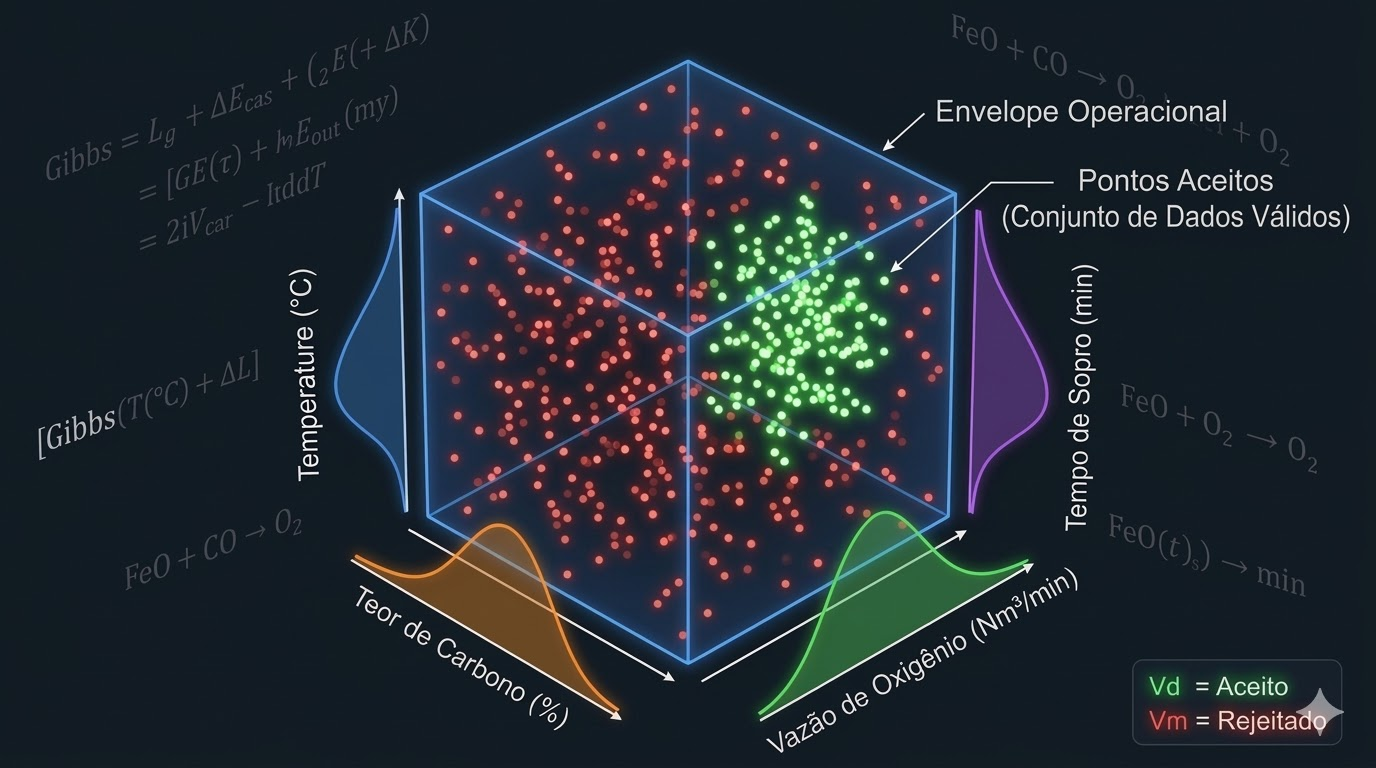
\includegraphics[width=0.60\textwidth]{Images/MonteCarlo}
\caption{Envelope operacional tridimensional da amostragem Monte Carlo para o dataset BOF sintético. Pontos verdes representam amostras aceitas (fisicamente válidas); pontos vermelhos, amostras rejeitadas por violação do critério de balanço entálpico (Equação~\ref{eq:criterio-entalpico}). Ilustração gerada com auxílio de inteligência artificial (Nano Banana Pro~3).}
\label{fig:monte-carlo-envelope}
\end{figure}

\begin{figure}[htbp]
\centering
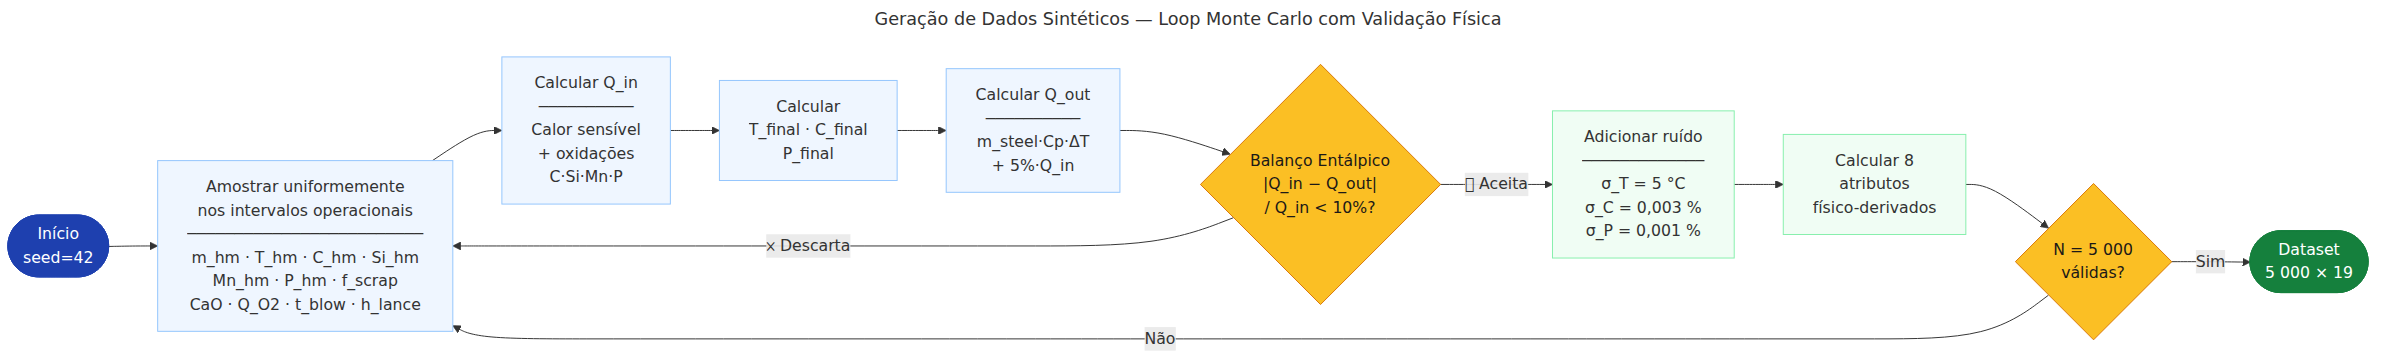
\includegraphics[width=0.88\textwidth,height=0.22\textheight,keepaspectratio]{Images/diagrams/02_monte_carlo_loop}
\caption{Fluxograma do loop de geração de dados sintéticos por Monte Carlo com validação de balanço entálpico. Amostras que violam o critério da Equação~\ref{eq:criterio-entalpico} são descartadas e o processo é repetido até $N = 10000$ instâncias válidas.}
\label{fig:monte-carlo-loop}
\end{figure}

\subsection{Atributos Físico-Derivados}
\label{subsec:feature-engineering}

A partir das variáveis brutas de cada instância, são calculados oito atributos físico-derivados com significado termodinâmico e estequiométrico direto\,\cite{chattopadhyay2022hybrid,shao2024hybrid,willard2020integrating}. Esses atributos condensam relações não-lineares entre variáveis de entrada que algoritmos puramente orientados a dados precisariam descobrir implicitamente a partir de exemplos\,\cite{cuomo2022physics}. A Tabela~\ref{tbl:features-fisicas} descreve cada atributo.

\begin{table}[H]
\centering
\caption{Atributos físico-derivados incorporados na Configuração~C}
\label{tbl:features-fisicas}
\small
\begin{tabular}{|p{3.8cm}|p{5.5cm}|p{4.7cm}|}
\hline
\textbf{Atributo} & \textbf{Fórmula (simplificada)} & \textbf{Significado físico} \\ \hline
\texttt{theo\_o2\_demand} & $m_\text{hm} \sum_i x_i \cdot r_i$ & O$_2$ mínimo para oxidar todas as impurezas \\ \hline
\texttt{o2\_efficiency} & $\text{theo\_o2} / (Q_{O_2} \cdot t_\text{blow})$ & Taxa de utilização do O$_2$ soprado \\ \hline
\texttt{enthalpy\_surplus} & $Q_\text{in} - Q_\text{out,scrap}$ & Energia disponível para fundir sucata \\ \hline
\texttt{total\_oxidized\_mass} & $\sum_i \Delta x_i \cdot m_\text{hm}$ & Massa total removida do banho \\ \hline
\texttt{decarb\_rate} & $C_\text{hm} / t_\text{blow}$ & Demanda teórica de descarburação por minuto de sopro \\ \hline
\texttt{slag\_basicity} & $\text{CaO} / (\text{Si}_\text{hm} \cdot m_\text{hm} \cdot f)$ & Capacidade de remoção de fósforo \\ \hline
\texttt{scrap\_melt\_capacity} & $\text{enthalpy\_surplus} / (C_{p,\text{scrap}} \cdot \Delta T)$ & Máximo de sucata fundível \\ \hline
\texttt{fe\_oxidation\_loss} & $(O_{2,\text{real}} - \text{theo\_o2}) \cdot r_\text{Fe}$ & Ferro perdido para a escória \\ \hline
\end{tabular}
\end{table}

\begin{figure}[H]
\centering
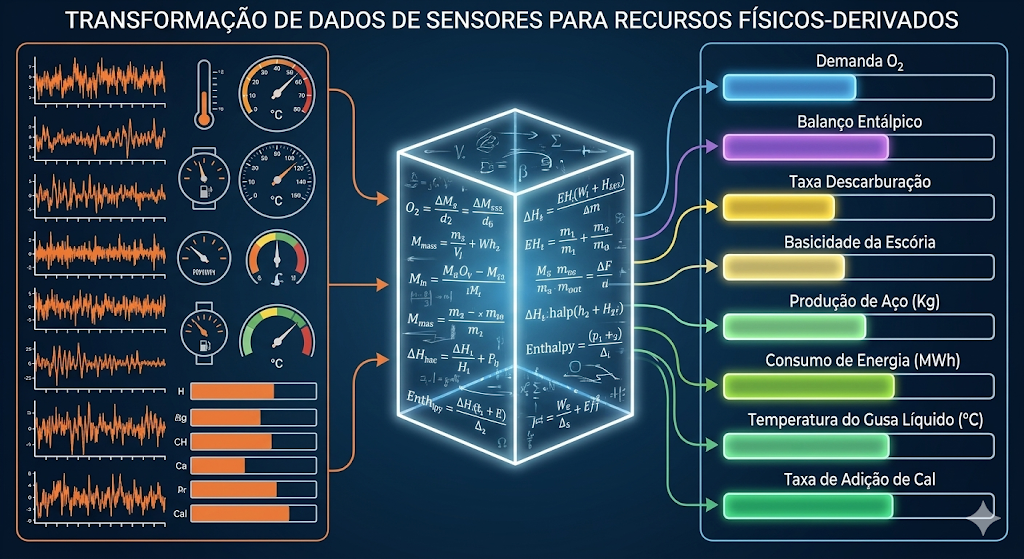
\includegraphics[width=0.65\textwidth]{Images/Raw_to_FeatureEngineered}
\caption{Transformação de dados brutos de sensores nos oito atributos físico-derivados: sinais de termopares, medidores de fluxo e espectrômetros (esquerda) são processados por balanços de massa e energia (centro), gerando grandezas com significado termodinâmico direto como demanda de O\textsubscript{2}, balanço entálpico, taxa de descarburação e basicidade da escória (direita). Ilustração gerada com auxílio de inteligência artificial (Nano Banana Pro~3).}
\label{fig:feature-engineering}
\end{figure}

%-------------------------------------------------------------------%
\section{Métodos}
\label{sec:metodos}

\subsection{Configurações Experimentais}
\label{subsec:configuracoes}

A metodologia proposta adota três configurações experimentais, permitindo isolar os efeitos da escolha de modelo e do conjunto de atributos\,\cite{zhou2024bof,he2021automl}:

\begin{itemize}
  \item \textbf{Config A — Linha de base}: modelos treinados exclusivamente com as variáveis brutas da Tabela~\ref{tbl:ranges-sinteticos}, com hiperparâmetros otimizados via Optuna\,\cite{akiba2019optuna} sobre o conjunto pré-definido de onze modelos da Tabela~\ref{tbl:modelos-ml} (implementação direta, sem uso de um framework de AutoML de portfólio como PyCaret ou Auto-sklearn\,\cite{he2021automl} — ver §\,\ref{subsec:otimizacao-treinamento}). Serve como referência para avaliar o ganho de desempenho das demais configurações.
  \item \textbf{Config B — Aprendizado profundo}: somente MLP com busca de arquitetura profunda via Optuna\,\cite{goodfellow2016deep,kingma2015adam}, treinada nas variáveis brutas. Isola o efeito da capacidade de representação da rede neural frente ao conjunto de modelos da Config~A.
  \item \textbf{Config C — Físico-informada}: mesmo conjunto completo de modelos da Config~A mais a MLP da Config~B, treinados no conjunto de variáveis brutas \emph{acrescido} dos oito atributos físico-derivados da Tabela~\ref{tbl:features-fisicas}\,\cite{xia2024dmpinn,willard2020integrating}. A comparação A$\times$C isola o efeito dos atributos físicos; A$\times$B isola o efeito da profundidade da rede; B$\times$C testa ambos simultaneamente.
\end{itemize}

\begin{figure}[H]
\centering
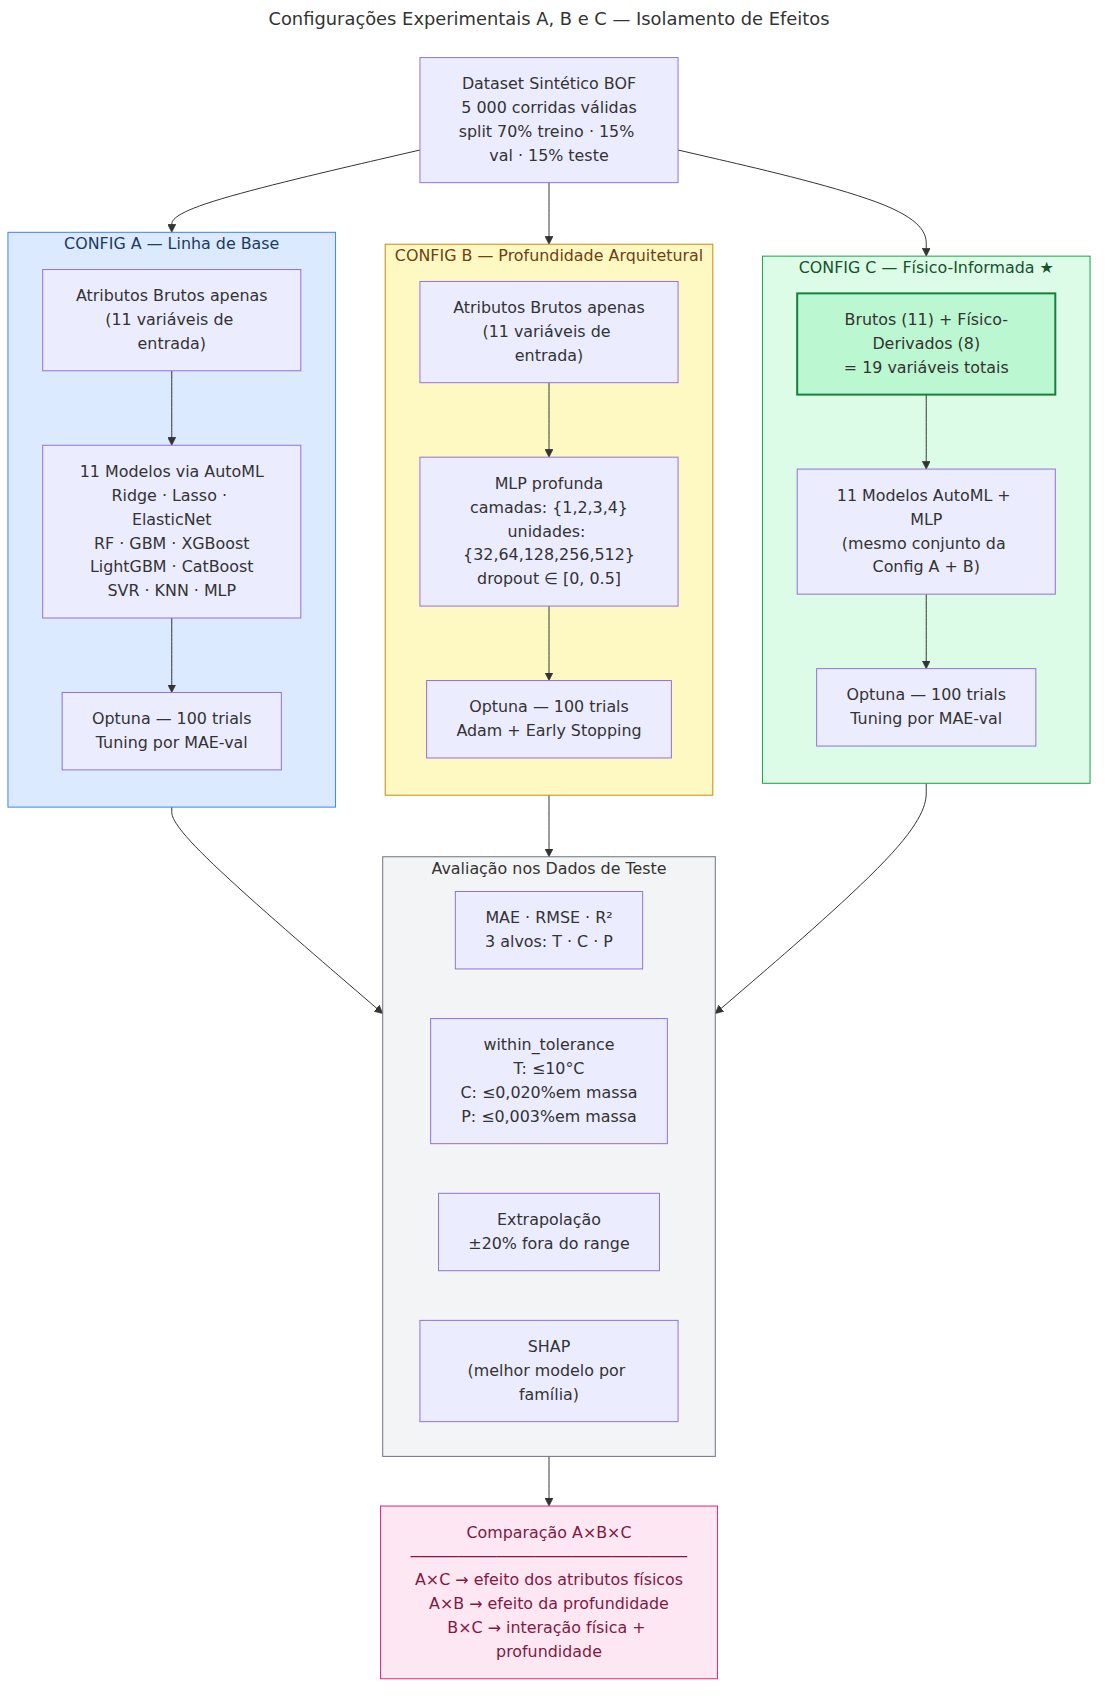
\includegraphics[width=0.80\textwidth,height=0.48\textheight,keepaspectratio]{Images/diagrams/04_experimental_configs}
\caption{Configurações experimentais A, B e~C: a Config~A serve como linha de base com atributos brutos; a Config~B isola o efeito da profundidade arquitetural da MLP; a Config~C incorpora os oito atributos físico-derivados ao mesmo conjunto de modelos da Config~A. A comparação cruzada A$\times$C, A$\times$B e B$\times$C permite isolar os efeitos de arquitetura e engenharia de atributos.}
\label{fig:experimental-configs}
\end{figure}

\begin{figure}[H]
\centering
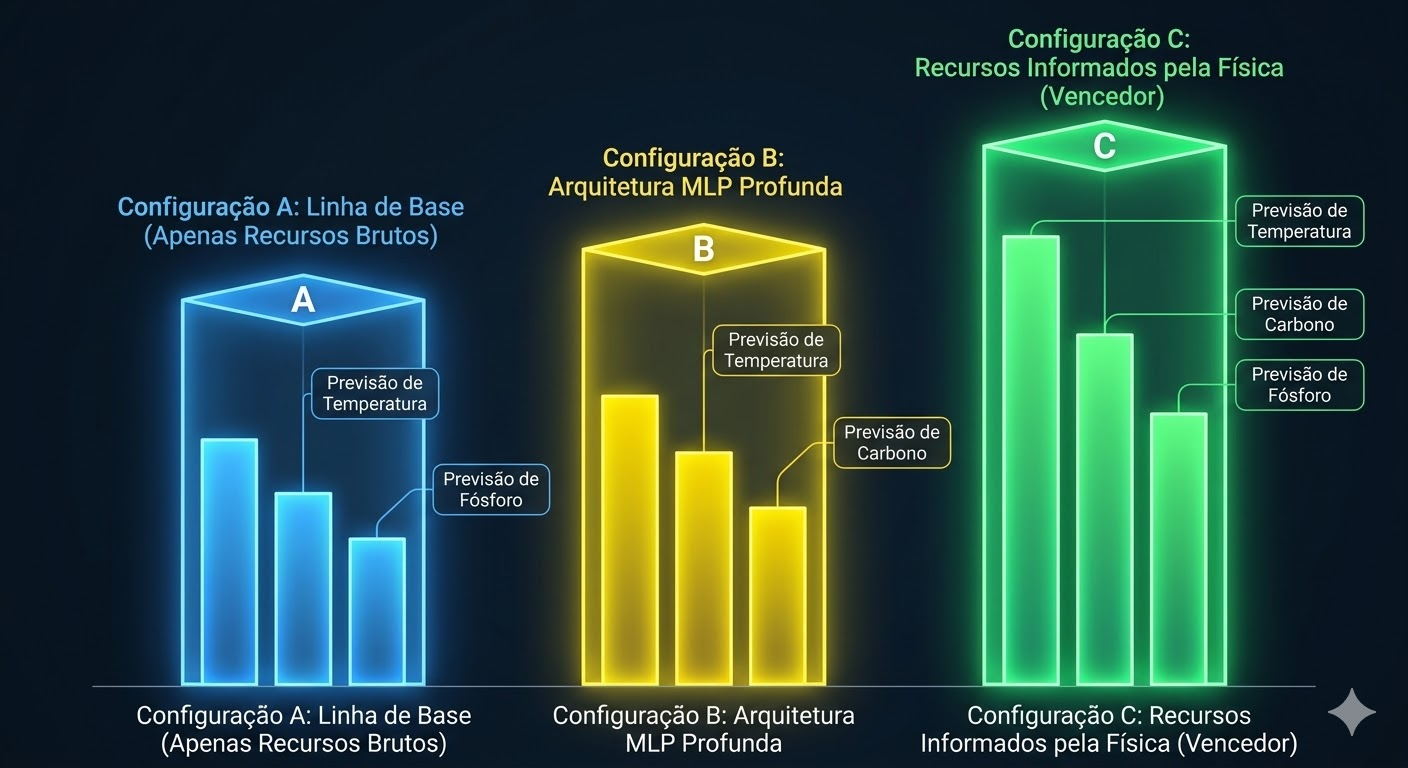
\includegraphics[width=0.60\textwidth]{Images/Configs}
\caption{Representação conceitual da hipótese de trabalho \emph{a priori}: a Config~C (físico-informada) melhoraria o desempenho nos três alvos frente às configurações A e~B. Os resultados reais (Capítulo~\ref{chp:resultados}) confirmam esse ganho para $[\text{C}]_\text{final}$ e $[\text{P}]_\text{final}$, mas não para $T_\text{final}$. Ilustração gerada com auxílio de inteligência artificial (Nano Banana Pro~3).}
\label{fig:configs-comparison}
\end{figure}

\subsection{Modelos de Regressão Supervisionada}
\label{subsec:modelos}

O conjunto de modelos avaliados nas Configs A e C é apresentado na Tabela~\ref{tbl:modelos-ml}. A seleção cobre as principais famílias de algoritmos de ML documentadas na literatura de predição de processos industriais\,\cite{zhou2024bof,chattopadhyay2022hybrid}.

\begin{table}[H]
\centering
\caption{Modelos de regressão supervisionada avaliados nas Configurações~A e~C}
\label{tbl:modelos-ml}
\small
\begin{tabular}{|p{3.0cm}|p{2.8cm}|p{8.2cm}|}
\hline
\textbf{Modelo} & \textbf{Família} & \textbf{Justificativa e referência} \\ \hline
Ridge & Linear L2 & Regularização $\ell_2$ reduz variância em espaços de alta dimensão\,\cite{hoerl1970ridge} \\ \hline
Lasso & Linear L1 & Regularização $\ell_1$ induz esparsidade e seleção implícita de atributos\,\cite{tibshirani1996regression} \\ \hline
ElasticNet & Linear L1+L2 & Combina vantagens de Ridge e Lasso; eficaz quando features são correlacionadas\,\cite{zou2005regularization} \\ \hline
Random Forest & Ensemble bagging & Boa capacidade de capturar não-linearidades sem overfitting excessivo\,\cite{breiman2001randomforests}; amplamente avaliado em predição de endpoint BOF\,\cite{zhou2024bof,chattopadhyay2022hybrid} \\ \hline
Gradient Boosting & Ensemble boosting & Boosting gradiente para regressão\,\cite{friedman2001greedy}, amplamente adotado em problemas industriais\,\cite{zhou2024bof} \\ \hline
XGBoost & Boosting otimizado & Regularização adicional e desempenho computacional superior a GBM padrão\,\cite{chen2016xgboost}; avaliado em predição de endpoint BOF\,\cite{zhou2024bof} \\ \hline
LightGBM & Boosting eficiente & Crescimento por folha com baixo consumo de memória para datasets médios\,\cite{ke2017lightgbm}; avaliado em predição de endpoint BOF\,\cite{zhou2024bof} \\ \hline
CatBoost & Boosting robusto & Tratamento nativo de variáveis categóricas; robusto a hiperparâmetros padrão\,\cite{prokhorenkova2018catboost}; avaliado em predição de endpoint BOF\,\cite{zhou2024bof} \\ \hline
SVR & Kernel & Eficaz em datasets de tamanho moderado com margem de insensibilidade ao ruído\,\cite{widodo2007svm} \\ \hline
KNN & Baseado em instâncias & Referência simples não-paramétrica; útil para verificar localidade do problema\,\cite{bishop2006prml} \\ \hline
MLP & Rede neural & Capacidade de aproximação universal; base da Config~B com busca profunda de arquitetura\,\cite{goodfellow2016deep} \\ \hline
\end{tabular}
\end{table}

\subsection{Protocolo de Treinamento e Avaliação}
\label{subsec:protocolo}

O protocolo de treinamento é idêntico para todas as configurações, garantindo comparabilidade. O dataset é dividido aleatoriamente em 70\,\% treino, 15\,\% validação e 15\,\% teste (seed=42)\,\cite{kohavi1995study} — sem estratificação, uma vez que os três alvos são variáveis contínuas e a amostragem de entrada já é aproximadamente uniforme (§\,\ref{subsec:preprocessamento}). A otimização de hiperparâmetros é realizada com o framework Optuna\,\cite{akiba2019optuna} sobre um conjunto pré-definido de modelos (Tabela~\ref{tbl:modelos-ml}), adotando 20 \textit{trials} por modelo por alvo — valor selecionado para equilibrar qualidade de busca e custo computacional com $N = 10000$ amostras; benchmarks em regressão tabular indicam retornos decrescentes além de 20--30 avaliações para espaços de hiperparâmetros de dimensão moderada\,\cite{he2021automl} —, amostrador TPE (\textit{Tree-structured Parzen Estimator})\,\cite{bergstra2011tpe} e objetivo de minimizar o MAE médio de validação cruzada com $k = 3$ folds sobre o conjunto de treino\,\cite{kohavi1995study} — valor de $k$ reduzido de 5 para conter o custo computacional total do protocolo (72 combinações modelo$\times$config$\times$alvo, 20 \textit{trials} cada). A partição de validação (15\,\%) é reservada na divisão do dataset mas, na versão atual do pipeline, não é consumida por nenhuma etapa do protocolo — nem o \textit{tuning} (que usa validação cruzada sobre o treino), nem a seleção de modelo final, nem as métricas reportadas neste capítulo, que se baseiam exclusivamente no conjunto de teste; a partição permanece disponível para uso futuro como critério de parada antecipada ou seleção hold-out independente da validação cruzada.

Para a Config~B, a busca de arquitetura da MLP percorre: número de camadas ocultas $\in \{1, 2, 3, 4\}$, unidades por camada $\in [32, 512]$ (inteiro, busca contínua) e taxa de aprendizado $\in [10^{-4}; 10^{-2}]$ — faixas consistentes com práticas consolidadas para redes neurais em regressão de processos industriais\,\cite{goodfellow2016deep,chattopadhyay2022hybrid} —, com regularização $\ell_2$ (\texttt{alpha})\,\cite{hoerl1970ridge}, otimizador Adam\,\cite{kingma2015adam} e \textit{early stopping} com paciência de 20 épocas.

As métricas de avaliação nos dados de teste são\,\cite{bishop2006prml}:

\begin{itemize}
  \item MAE — Erro Médio Absoluto: métrica principal, diretamente comparável aos limiares industriais;
  \item RMSE — Raiz do Erro Quadrático Médio: penaliza erros grandes, relevante para robustez;
  \item R$^2$ — Coeficiente de Determinação: proporção da variância explicada pelo modelo;
  \item \texttt{within\_tolerance}: fração das predições de teste dentro do limiar industrial de qualidade — $\leq 10$\,°C para T\textsubscript{final}, $\leq 0{,}020$\,\%~em~massa para C\textsubscript{final} e $\leq 0{,}003$\,\%~em~massa para P\textsubscript{final}\,\cite{zhou2024bof,bae2020bof}.
\end{itemize}

Adicionalmente, é realizado um teste de extrapolação: 500 amostras, cada uma com uma variável de entrada (escolhida aleatoriamente, independentemente por amostra, entre as 14 disponíveis) deslocada além do seu limite de treino por uma fração aleatória entre 2\,\% e 20\,\% da largura da faixa dessa variável (média $\approx 11\,\%$; não um deslocamento fixo de 20\,\%), são avaliadas nos modelos já treinados. O valor-alvo verdadeiro é recalculado pelo mesmo modelo físico usado na geração dos dados, aplicado às entradas perturbadas --- não um substituto do conjunto de teste em distribuição, o que mediria divergência frente a valores de referência não relacionados às entradas perturbadas, e não erro de extrapolação real. Esse recálculo verifica se a incorporação de atributos físico-derivados melhora a generalização fora do domínio de treinamento; como a função geradora subjacente é a mesma dentro e fora da faixa de amostragem, o teste mede erro de emulação sob extensão da caixa de amostragem, não robustez a um regime físico genuinamente distinto\,\cite{bae2020bof}. A análise SHAP\,\cite{lundberg2017unified,manojlovic2022eaf} é aplicada a três modelos representativos de famílias distintas da Config~C (ensemble de bagging, \textit{boosting} e rede neural) --- não necessariamente os de menor MAE em cada alvo individualmente ---, verificando se os atributos físico-derivados apresentam alta importância e se a direção de influência é fisicamente coerente.

\textbf{Ambiente computacional.} Os experimentos foram executados em sistema Linux (WSL2) com 16 núcleos lógicos e 17\,GB de RAM, com aceleração por GPU (NVIDIA GeForce RTX 5060 Laptop) utilizada pelos treinadores nativos de XGBoost e CatBoost. O ambiente Python\,3.13 utiliza as seguintes bibliotecas principais: scikit-learn\,1.7, XGBoost\,3.1, LightGBM\,4.6, CatBoost\,1.2, Optuna\,4.7, SHAP\,0.51 e NumPy\,2.3. O código de geração de dados, engenharia de atributos e treinamento está disponível no repositório do projeto, garantindo reprodutibilidade integral dos experimentos\,\cite{buggineni2024synthetic}.

\subsection{Ameaças à Validade}
\label{subsec:ameacas-validade}

Três ameaças estruturais condicionam a interpretação dos resultados e devem ser explicitadas antes da análise comparativa.

\textbf{Separação estrutural entre gerador e atributos físico-derivados.}
A versão ingênua deste protocolo sofreria de circularidade severa: se o gerador de dados e o cálculo de atributos utilizassem exatamente as mesmas equações e constantes, os atributos físico-derivados seriam transformações algébricas quase-determinísticas dos alvos.
Por exemplo, o $T_\text{final}$ é determinado por $Q_\text{in} \times \eta_\text{eff} - Q_\text{scrap}$; se o atributo \texttt{enthalpy\_surplus} utilizasse a mesma $\eta_\text{eff}$, um modelo linear teria acesso ao alvo via inversão direta da fórmula.

Para eliminar essa patologia, adotou-se um protocolo de \textbf{separação por dois níveis de modelagem física}, descrito a seguir:

\begin{description}
  \item[Nível~1 — Gerador (processo real simulado):] cada amostra tem constantes físicas específicas à corrida, amostradas de distribuições calibradas pela literatura: constante de descarburação $k \sim \mathcal{N}(78{,}0;\, 12\%)$, eficiência térmica $\eta_\text{eff} \sim \mathcal{N}(0{,}64;\, 6\%)$, frações de remoção de C, Si, Mn e P com coeficientes de variação de 3–10\%\,\cite{chattopadhyay2022hybrid,logar2022eaf}. Essas constantes específicas à corrida representam variações reais de desgaste de lança, condição refratária e viscosidade de escória --- grandezas não observáveis pelas entradas do modelo de controle de processo.
  \item[Nível~2 — Atributos (estimativa de engenharia publicada):] \texttt{calc\_physics\_features} emprega constantes \emph{fixas} da literatura, com oxidação teórica completa (frações de remoção iguais a~1,0) e sem correção CO/CO$_2$ --- o que tabelas termodinâmicas publicadas reportam como liberação de calor bruta máxima. A eficiência térmica $\eta_\text{eff}$ não é aplicada nos atributos, simulando o que um engenheiro calcula \emph{antes} da corrida a partir de tabelas padrão.
\end{description}

A consequência prática é que \texttt{enthalpy\_surplus} e $T_\text{final}$ são correlacionados, mas \textbf{não algebricamente equivalentes}: a variabilidade em $\eta_\text{eff}$ e nas frações de remoção introduz uma discrepância estruturada entre a estimativa do atributo e o alvo gerado. O mesmo padrão aplica-se a \texttt{total\_oxidized\_mass} (teórica vs.\ parcial calibrada) e à relação \texttt{slag\_basicity}–$[\text{P}]_\text{final}$ (coeficiente de partição específico à corrida vs.\ fórmula publicada fixa)\,\cite{bae2020bof}.

A informação mútua normalizada $I(f; y) / H(y_\text{std})$, onde $H(y_\text{std}) = 0{,}5\ln(2\pi e)$ é a entropia diferencial do alvo padronizado, entre cada atributo físico-derivado e cada alvo será reportada no Capítulo~\ref{chp:resultados} como medida quantitativa do grau de associação residual após a separação, segundo a escala de interpretação pré-definida: NMI $< 0{,}30$ (associação baixa), $0{,}30$--$0{,}60$ (moderada, atributo informativo mas não determinístico), $0{,}60$--$0{,}85$ (alta, vínculo estrutural forte) e $> 0{,}85$ (quase-determinística, indício de circularidade residual). A avaliação de robustez dos ganhos de Config~C sob perturbação deliberada das constantes termodinâmicas dos atributos — simulando mismatch sistemático entre o modelo de engenharia e o processo real — constitui uma extensão natural para trabalhos futuros\,\cite{buggineni2024synthetic,willard2020integrating}.

\textbf{Definição do atributo \texttt{decarb\_rate} e sua limitação.}
O atributo é definido como $C_\text{hm} / t_\text{blow}$ — carbono inicial do gusa por unidade de tempo de sopro, calculável exclusivamente de variáveis de entrada conhecidas antes do sopro. A alternativa $(C_\text{hm} - C_\text{final}) / t_\text{blow}$ constituiria vazamento de dados: $C_\text{final}$ é variável-alvo desconhecida no momento da predição\,\cite{chattopadhyay2022hybrid,bae2020bof}.

Essa escolha defensiva tem um custo físico reconhecido: \texttt{decarb\_rate} captura a carga inicial de carbono por minuto de sopro, não a dinâmica real de remoção ao longo da corrida. Dados contínuos de lança — vazão instantânea de O$_2$ integrada, perfil de posição de lança — permitiriam construir um atributo mais informativo sobre a cinética de descarburação, mas não estão disponíveis como entradas do modelo no instante de predição de \textit{endpoint}. A limitação não é exclusiva desta dissertação: é inerente a qualquer sistema de predição sem acesso a medições em tempo real durante o sopro.

\textbf{Amostragem uniforme independente.} As variáveis de entrada são amostradas de distribuições uniformes independentes (Tabela~\ref{tbl:ranges-sinteticos}), desconsiderando correlações operacionais reais --- por exemplo, gusa com alto teor de Si tipicamente induz ajustes correlacionados na adição de cal e no perfil de sopro. Amostragem baseada em cópulas ou modelos de mistura capturaria melhor a distribuição conjunta real, mas exigiria dados industriais para calibração\,\cite{morales2025synthetic}. A distribuição uniforme é uma escolha conservadora que maximiza a cobertura do espaço operacional ao custo de incluir combinações operacionalmente improváveis.

\begin{figure}[H]
\centering
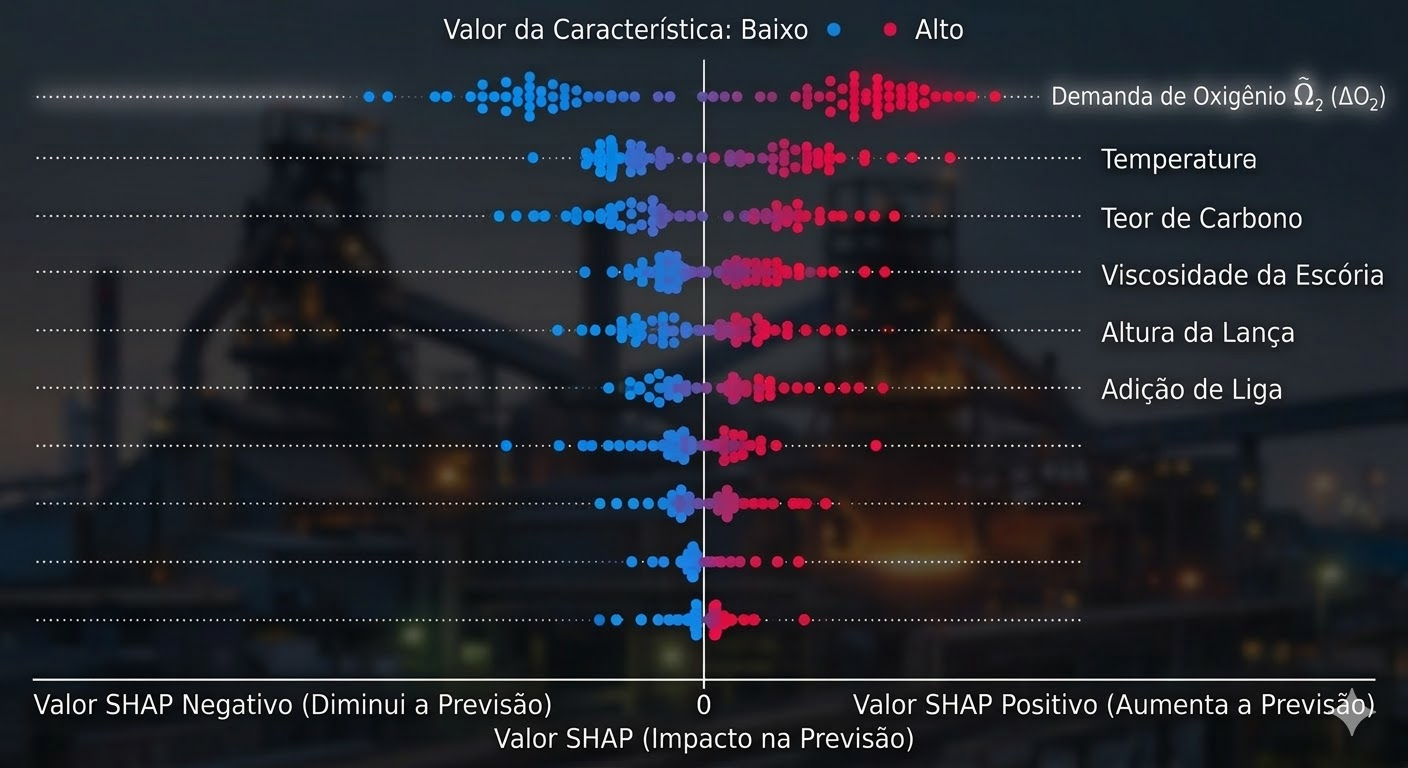
\includegraphics[width=0.65\textwidth]{Images/SHAP}
\caption{\textit{Beeswarm plot} SHAP conceitual: cada ponto representa a contribuição de um atributo para uma predição individual. Pontos à direita (vermelho) indicam impacto positivo na predição; à esquerda (azul), impacto negativo. A eficiência de consumo de O\textsubscript{2} (\texttt{o2\_efficiency}) é o atributo físico-derivado de maior importância para $[\text{C}]_\text{final}$ nos três modelos testados (Capítulo~\ref{chp:resultados}), em linha com o conhecimento metalúrgico de que a reação $\text{C} + \tfrac{1}{2}\text{O}_2 \rightarrow \text{CO}$ governa a descarburação. Ilustração gerada com auxílio de inteligência artificial (Nano Banana Pro~3).}
\label{fig:shap-beeswarm}
\end{figure}

\begin{figure}[H]
\centering
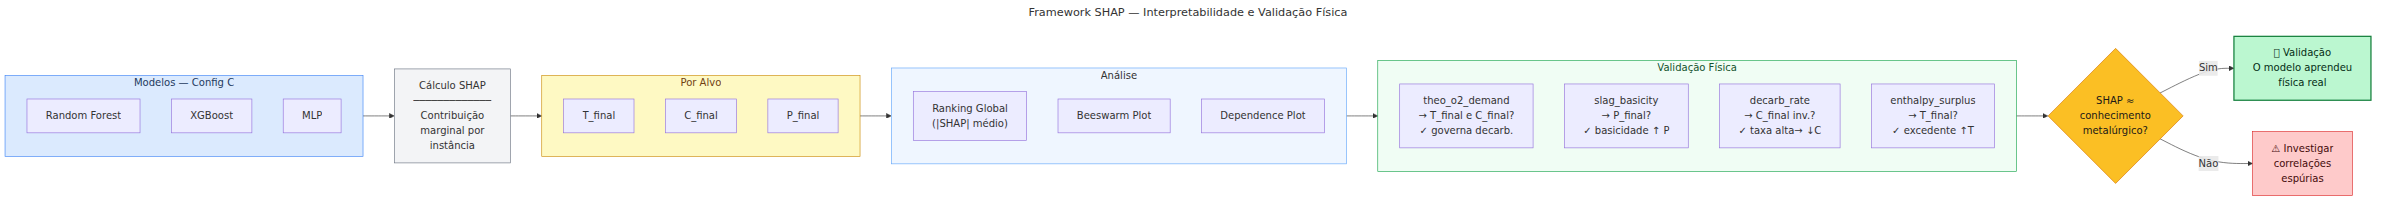
\includegraphics[width=0.88\textwidth]{Images/diagrams/06_shap_validation}
\caption{Framework de validação física por SHAP: os modelos treinados na Config~C são submetidos a análise SHAP por variável-alvo, gerando rankings de importância e gráficos de dependência. A consistência dos resultados com o conhecimento metalúrgico (\textit{e.g.}, basicidade da escória entre os atributos mais relevantes para P) é compatível com --- sem provar --- a captura de estrutura física pelo modelo; o Capítulo~\ref{chp:resultados} reporta que 4 das 5 hipóteses pré-registradas não foram falsificadas.}
\label{fig:shap-validation}
\end{figure}

\chapter{Resultados e Discussão}
\label{chp:resultados}

Este capítulo apresenta os resultados experimentais da tarefa de regressão supervisionada nas três configurações do pipeline, todas integralmente concluídas, e a análise de interpretabilidade via SHAP sobre os melhores modelos da Config~C. Os resultados de Config~A (linha de base, atributos brutos, 11 modelos), Config~B (MLP profundo com busca de arquitetura via Optuna, atributos brutos) e Config~C (física informada, atributos brutos mais os oito físico-derivados, 12 modelos) são reportados com MAE, RMSE, $R^2$ e fração de predições dentro da tolerância industrial ($w_\text{tol}$). A comparação A~vs.~C é testada com o teste de Wilcoxon com postos assinados sobre os 1.500 erros absolutos pareados do conjunto de teste\,\cite{demsar2006statistical}. Ao total foram treinados e avaliados 33 combinações (modelo $\times$ alvo) para a Config~A, 3 para a Config~B e 36 para a Config~C, perfazendo 72 modelos otimizados via Optuna com 20 \textit{trials} cada. O tempo total, da geração de dados aos resultados de SHAP e circularidade aqui reportados, foi de aproximadamente 10\,h\,29\,min no ambiente computacional descrito no Capítulo~\ref{chp:capitulo4}, com o treinamento dos modelos (etapa 3) dominando o tempo total e a busca de arquitetura profunda do MLP (Configs~B e~C) sendo a mais custosa por modelo individual.

\section{Config~A: Linha de Base com Atributos Brutos}
\label{sec:resultados-A}

Os resultados completos de Config~A são exibidos na Tabela~\ref{tbl:resultados_configA}. MAE em negrito indica cumprimento do limiar industrial.

\begin{table}[H]
\caption{Config~A --- atributos brutos, 11 modelos. MAE em negrito: cumpre limiar industrial ($T_\text{final} \leq 10\,^\circ\text{C}$; $[\text{C}]_\text{final} \leq 0{,}020\,\%$; $[\text{P}]_\text{final} \leq 0{,}003\,\%$)~\cite{zhou2024bof,bae2020bof}. $w_\text{tol}$: fração de predições dentro da tolerância. Dataset $N=10{.}000$; partição 70/15/15\,\%; Optuna 20 \textit{trials}/modelo/alvo.}
\label{tbl:resultados_configA}
\centering
\footnotesize
\setlength{\tabcolsep}{4pt}
\begin{tabular}{lrrrrrrrrrr}
\hline
\textbf{Modelo} &
  \multicolumn{3}{c}{$T_\text{final}$ (°C)} &
  \multicolumn{3}{c}{$[\text{C}]_\text{final}$ (\%)} &
  \multicolumn{3}{c}{$[\text{P}]_\text{final}$ (\%)} \\
\cline{2-4}\cline{5-7}\cline{8-10}
 & MAE & $R^2$ & $w_\text{tol}$ & MAE & $R^2$ & $w_\text{tol}$ & MAE & $R^2$ & $w_\text{tol}$ \\
\hline
Ridge      & 23,91 & 0,367 & 22,2\,\% & \textbf{0,0156} & 0,711 & 66,3\,\% & 0,00326 & 0,601 & 53,9\,\% \\
Lasso      & 23,91 & 0,367 & 22,2\,\% & \textbf{0,0156} & 0,711 & 66,5\,\% & 0,00327 & 0,600 & 53,3\,\% \\
ElasticNet & 23,91 & 0,367 & 22,2\,\% & \textbf{0,0156} & 0,711 & 66,5\,\% & 0,00326 & 0,601 & 54,1\,\% \\
RF         & 23,45 & 0,351 & 25,0\,\% & \textbf{0,0093} & 0,823 & 85,1\,\% & 0,00304 & 0,641 & 58,6\,\% \\
GBM        & 23,43 & 0,342 & 26,4\,\% & \textbf{0,0093} & 0,816 & 84,7\,\% & 0,00301 & 0,641 & 59,1\,\% \\
XGBoost    & 23,24 & 0,356 & 25,5\,\% & \textbf{0,0096} & 0,825 & 84,9\,\% & 0,00302 & 0,641 & 59,1\,\% \\
LightGBM   & 23,08 & 0,338 & 29,7\,\% & \textbf{0,0088} & 0,831 & 85,7\,\% & 0,00300 & 0,646 & 59,4\,\% \\
CatBoost   & 23,25 & 0,365 & 26,5\,\% & \textbf{0,0094} & 0,832 & 83,7\,\% & \textbf{0,00299} & 0,648 & 58,9\,\% \\
SVR        & 21,86 & 0,347 & 35,9\,\% & \textbf{0,0129} & 0,771 & 78,1\,\% & 0,00348 & 0,546 & 49,3\,\% \\
KNN        & 26,00 & 0,254 & 18,8\,\% & \textbf{0,0157} & 0,635 & 67,9\,\% & 0,00355 & 0,546 & 46,9\,\% \\
MLP        & 24,88 & 0,309 & 22,1\,\% & \textbf{0,0091} & 0,840 & 84,5\,\% & 0,00314 & 0,626 & 55,3\,\% \\
\hline
\end{tabular}
\end{table}

Os resultados da Config~A revelam uma hierarquia de dificuldade marcada entre os três alvos. $[\text{C}]_\text{final}$ é o alvo mais bem capturado pelos atributos brutos: todos os onze modelos atendem ao limiar de 0{,}020\,\%, com os ensembles de árvore e o MLP (RF, GBM, XGBoost, LightGBM, CatBoost, MLP) alcançando MAE entre 0{,}0088\,\% e 0{,}0096\,\% e $R^2$ até 0{,}840. Isso indica que as variáveis brutas --- especialmente $[\text{C}]_\text{hm}$ e $\dot{V}_{\text{O}_2}$ --- já codificam suficientemente a relação exponencial de descarburação.

$T_\text{final}$ é o alvo discriminante: nenhum dos onze modelos atinge o limiar de $10\,^\circ\text{C}$, com MAE variando entre $21{,}86\,^\circ\text{C}$ (SVR) e $26{,}00\,^\circ\text{C}$ (KNN) e $R^2$ entre 0{,}254 e 0{,}367. Este resultado merece interpretação cuidadosa: o limiar de $10\,^\circ\text{C}$ adotado na literatura~\cite{xia2024dmpinn,bae2020bof} pressupõe a disponibilidade de informação temporal durante o sopro (perfis de off-gas, medições de sublança intermediárias), que são inacessíveis a um modelo estático pré-sopro como o desta dissertação. A questão não é se os modelos falharam, mas sim qual é o limite informacional-teórico da predição com variáveis exclusivamente pré-sopro. O $R^2$ entre 0{,}25 e 0{,}37 reflete, em parte, a variância irredutível imposta por $\eta_\text{eff} \sim \mathcal{N}(0{,}64;\,6\%)$, uma grandeza estocástica por corrida não observável nas features de entrada --- análogo ao ruído de Bayes em classificação\,\cite{bishop2006prml,goodfellow2016deep}; essa variância estabelece um teto teórico que nenhum modelo supervisionado pode ultrapassar com os atributos disponíveis. Mas parte do $R^2$ reportado também é inflada pela censura de $T_\text{final}$ nos limites da faixa-alvo (Capítulo~\ref{chp:capitulo4}, $40{,}5\,\%$ das amostras): recalculando sobre o subconjunto de teste não saturado, o $R^2$ do SVR (Config~A) cai de $0{,}347$ para $0{,}240$, enquanto o MAE se mantém praticamente inalterado ($21{,}86\,^\circ\text{C}$ vs.\ $22{,}00\,^\circ\text{C}$) --- ou seja, a censura reduz artificialmente a variância total a explicar sem tornar a predição pontual mais fácil.

$[\text{P}]_\text{final}$ constitui o segundo alvo crítico: apenas o CatBoost atinge o limiar de 0{,}003\,\% (MAE~$=0{,}002993\,\%$, margem mínima), com os demais ensembles em MAE~$\approx 0{,}0030\,\%$ --- fração de um por cento acima --- e $w_\text{tol}$ entre 58{,}6\,\% e 59{,}4\,\%. O $R^2$ (0{,}55--0{,}65) reflete a dificuldade de inferir a basicidade efetiva da escória sem o atributo combinado \texttt{slag\_basicity}: a remoção de fósforo é função fortemente não-linear desta variável~\cite{bae2020bof,chattopadhyay2022hybrid}.

A convergência dos três modelos lineares (Ridge, Lasso, ElasticNet) em desempenho quase idêntico confirma que o gargalo nessa família é estrutural --- incapacidade de capturar interações de segunda ordem --- e não hiperparamétrico. Esse é precisamente o cenário onde atributos físico-derivados pré-computados têm maior impacto esperado~\cite{willard2020integrating,chattopadhyay2022hybrid}.


\section{Config~B: MLP Profundo com Atributos Brutos}
\label{sec:resultados-B}

A Config~B avalia se a profundidade arquitetural do MLP, com busca automática de número de camadas e neurônios via Optuna, é suficiente para superar os ensembles da linha de base sem atributos físico-derivados. Os resultados são exibidos na Tabela~\ref{tbl:resultados_configB}.

\begin{table}[H]
\caption{Config~B --- MLP profundo (\texttt{mlp\_deep}) com atributos brutos. Busca de arquitetura via Optuna (20 \textit{trials}); os demais protocolos são idênticos à Config~A.}
\label{tbl:resultados_configB}
\centering
\footnotesize
\setlength{\tabcolsep}{5pt}
\begin{tabular}{lrrrrrrrrrr}
\hline
\textbf{Modelo} &
  \multicolumn{3}{c}{$T_\text{final}$ (°C)} &
  \multicolumn{3}{c}{$[\text{C}]_\text{final}$ (\%)} &
  \multicolumn{3}{c}{$[\text{P}]_\text{final}$ (\%)} \\
\cline{2-4}\cline{5-7}\cline{8-10}
 & MAE & $R^2$ & $w_\text{tol}$ & MAE & $R^2$ & $w_\text{tol}$ & MAE & $R^2$ & $w_\text{tol}$ \\
\hline
MLP$_\text{deep}$ & 24,03 & 0,342 & 23,5\,\% & \textbf{0,0090} & 0,839 & 84,5\,\% & 0,0032 & 0,608 & 55,3\,\% \\
\hline
\end{tabular}
\end{table}

A Config~B não supera os melhores modelos da Config~A em nenhum dos três alvos: o MLP profundo obtém MAE$_{T} = 24{,}03\,^\circ\text{C}$ contra $21{,}86\,^\circ\text{C}$ do SVR --- o melhor modelo da Config~A para este alvo --- e frente aos ensembles de árvore (23{,}08--23{,}45\,\textdegree C) também não há ganho. Para $[\text{C}]_\text{final}$ e $[\text{P}]_\text{final}$ o MLP profundo é comparável, mas não superior, aos modelos de boosting. Esse resultado é consistente com a literatura sobre dados tabulares de domínio industrial, onde gradiente-boosting tende a superar redes neurais rasas e profundas quando o número de amostras é da ordem de $10^4$ e as relações entre variáveis não têm estrutura espacial ou temporal explorada por convoluções ou recorrências~\cite{grinsztajn2022tree,shwartz2022tabular}. A implicação prática é que, no domínio BOF com dados tabulares estáticos, investir em profundidade arquitetural sem incorporar conhecimento físico não produz ganho preditivo.


\section{Config~C: Física Informada com Oito Atributos Físico-Derivados}
\label{sec:resultados-C}

A Config~C expande o espaço de atributos com os oito físico-derivados descritos no Capítulo~\ref{chp:capitulo4}. Os resultados completos são exibidos na Tabela~\ref{tbl:resultados_configC}.

\begin{table}[H]
\caption{Config~C --- atributos brutos + 8 físico-derivados, 12 modelos. Mesmas convenções da Tabela~\ref{tbl:resultados_configA}.}
\label{tbl:resultados_configC}
\centering
\footnotesize
\setlength{\tabcolsep}{4pt}
\begin{tabular}{lrrrrrrrrrr}
\hline
\textbf{Modelo} &
  \multicolumn{3}{c}{$T_\text{final}$ (°C)} &
  \multicolumn{3}{c}{$[\text{C}]_\text{final}$ (\%)} &
  \multicolumn{3}{c}{$[\text{P}]_\text{final}$ (\%)} \\
\cline{2-4}\cline{5-7}\cline{8-10}
 & MAE & $R^2$ & $w_\text{tol}$ & MAE & $R^2$ & $w_\text{tol}$ & MAE & $R^2$ & $w_\text{tol}$ \\
\hline
Ridge          & 23,90 & 0,368 & 21,7\,\% & \textbf{0,0131} & 0,766 & 77,2\,\% & 0,00324 & 0,602 & 53,9\,\% \\
Lasso          & 23,90 & 0,367 & 22,1\,\% & \textbf{0,0134} & 0,763 & 76,0\,\% & 0,00327 & 0,600 & 53,3\,\% \\
ElasticNet     & 23,90 & 0,367 & 22,1\,\% & \textbf{0,0131} & 0,766 & 76,9\,\% & 0,00325 & 0,602 & 53,9\,\% \\
RF             & 23,51 & 0,348 & 24,7\,\% & \textbf{0,0087} & 0,838 & 85,1\,\% & \textbf{0,00293} & 0,662 & 61,1\,\% \\
GBM            & 23,33 & 0,344 & 26,9\,\% & \textbf{0,0087} & 0,840 & 85,8\,\% & \textbf{0,00294} & 0,663 & 60,1\,\% \\
XGBoost        & 23,20 & 0,359 & 26,5\,\% & \textbf{0,0090} & 0,838 & 86,3\,\% & \textbf{0,00294} & 0,661 & 59,8\,\% \\
LightGBM       & 23,31 & 0,339 & 26,5\,\% & \textbf{0,0088} & 0,840 & 86,1\,\% & \textbf{0,00294} & 0,662 & 59,4\,\% \\
CatBoost       & 23,16 & 0,365 & 26,7\,\% & \textbf{0,0086} & 0,843 & 85,9\,\% & \textbf{0,00293} & 0,664 & 60,2\,\% \\
SVR            & 22,15 & 0,348 & 34,5\,\% & \textbf{0,0099} & 0,820 & 82,7\,\% & 0,00348 & 0,538 & 49,2\,\% \\
KNN            & 25,84 & 0,265 & 17,3\,\% & \textbf{0,0131} & 0,713 & 73,8\,\% & 0,00356 & 0,547 & 47,1\,\% \\
MLP            & 27,37 & 0,120 & 21,1\,\% & \textbf{0,0090} & 0,842 & 85,7\,\% & \textbf{0,00297} & 0,645 & 58,9\,\% \\
MLP$_\text{deep}$ & 25,06 & 0,269 & 22,9\,\% & \textbf{0,0088} & 0,844 & 85,5\,\% & 0,0030 & 0,646 & 58,9\,\% \\
\hline
\end{tabular}
\end{table}

Os resultados da Config~C evidenciam um padrão assimétrico entre os três alvos, que constitui a principal descoberta experimental desta dissertação.

Para $[\text{C}]_\text{final}$, os oito atributos físico-derivados produzem melhoria estatisticamente significativa pelo teste de Wilcoxon em 10 dos 11 pares A~vs.~C ($p < 0{,}05$; Tabela~\ref{tbl:wilcoxon_detail}) --- a exceção é o LightGBM ($p = 0{,}441$), cujo desempenho já era o melhor da Config~A e deixa pouca margem de ganho. Os modelos de gradiente-boosting atingem MAE entre 0{,}0086\,\% (CatBoost) e 0{,}0090\,\% (XGBoost) --- redução de até 8{,}7\,\% em relação à Config~A no CatBoost, mas de apenas 0{,}8\,\% no LightGBM (o único par não significativo desta lista) --- com $R^2$ até 0{,}843. Atributos como \texttt{o2\_efficiency} e \texttt{decarb\_rate} codificam relações termodinâmicas que os ensembles de árvore passam a acessar diretamente como divisões de nó, em vez de precisar reaprendê-las a partir de interações entre variáveis brutas~\cite{willard2020integrating,shao2024hybrid}.

Para $[\text{P}]_\text{final}$, oito dos 11 pares mostram melhoria significativa ($p \leq 0{,}028$; Tabela~\ref{tbl:wilcoxon_detail}) --- Lasso, SVR e KNN são as exceções não-significativas. O ganho mais notável é prático, não apenas estatístico: seis modelos (RF, GBM, XGBoost, LightGBM, CatBoost, MLP) passam a atender ao limiar industrial de 0{,}003\,\%, contra apenas um (CatBoost, por margem mínima) na Config~A. O melhor resultado é o CatBoost, com MAE~$= 0{,}002926\,\%$ --- $2{,}5\,\%$ abaixo do limiar. A incorporação de \texttt{slag\_basicity}, que condensa (CaO + MgO)/$\text{SiO}_2$ em um único atributo, desloca uma fração substancial dos modelos de fósforo para dentro da faixa de aceitação industrial~\cite{bae2020bof,chattopadhyay2022hybrid}.

O caso mais chamativo da Config~C é o MLP em $T_\text{final}$: seu MAE sobe de $24{,}88\,^\circ\text{C}$ (Config~A) para $27{,}37\,^\circ\text{C}$ (Config~C), com $R^2$ caindo de $0{,}309$ para $0{,}120$ --- a maior degradação observada em toda a comparação. De forma mais geral, nenhum modelo da Config~C apresenta melhoria estatisticamente significativa para $T_\text{final}$ (Tabela~\ref{tbl:wilcoxon_detail}): os atributos físico-derivados não resolvem o gargalo deste alvo. Como o teste de Wilcoxon aqui aplicado é unilateral (testa apenas se C é melhor que A), ele não pode, por construção, atestar significância estatística para uma piora; a degradação do MLP é, portanto, relatada como observação descritiva direta das métricas (não como resultado de teste de hipótese) e é consistente com dificuldades conhecidas de convergência de redes neurais quando a dimensionalidade de entrada aumenta sem crescimento proporcional do conjunto de treino~\cite{goodfellow2016deep,grinsztajn2022tree}. Esses resultados confirmam o teto informacional discutido na Seção~\ref{sec:resultados-A}: a variância irredutível de $\eta_\text{eff}$ limita o ganho possível para $T_\text{final}$ independentemente da estratégia de atributos.

Os modelos lineares apresentam ganho relevante em $[\text{C}]_\text{final}$ na Config~C ($\Delta$MAE entre $-0{,}0022$ e $-0{,}0025\,\%$, todos significativos), confirmando que os atributos físico-derivados linearizam interações antes inacessíveis a regressores sem termos de interação explícitos. Para $T_\text{final}$, o ganho linear é nulo; para $[\text{P}]_\text{final}$, Ridge e ElasticNet melhoram significativamente, mas Lasso não --- provavelmente por zerar o coeficiente de algum atributo físico-derivado durante a regularização $L_1$.


\section{Comparação Estatística A~vs.~C}
\label{sec:comparacao-ac}

A Tabela~\ref{tbl:wilcoxon_summary} sintetiza os resultados do teste de Wilcoxon por alvo. O tamanho de efeito $r = Z / \sqrt{N}$ quantifica a magnitude prática das diferenças além do critério binário de significância~\cite{field2009discovering}.

\begin{table}[H]
\caption{Síntese do teste de Wilcoxon (A~vs.~C) por alvo. $n_\text{sig}$: modelos com melhoria significativa em C ($p < 0{,}05$). $\bar{r}$: tamanho de efeito médio (pares significativos; ``---'' quando não há par significativo). $\Delta$MAE: diferença MAE$_C$ $-$ MAE$_A$ do modelo com menor MAE$_C$ (negativo = C melhor).}
\label{tbl:wilcoxon_summary}
\centering
\footnotesize
\setlength{\tabcolsep}{6pt}
\begin{tabular}{lrrrl}
\hline
\textbf{Alvo} & $n_\text{sig}$ / 11 & $\bar{r}$ (sig.) & $\Delta$MAE (melhor MAE$_C$) & Direção \\
\hline
$T_\text{final}$  & 0  & --- & $+0{,}29\,^\circ\text{C}$ (SVR) & A~$\geq$~C \\
$[\text{C}]_\text{final}$ & 10 & 0,238 & $-0{,}00082\,\%$ (CatBoost) & C~$>$~A \\
$[\text{P}]_\text{final}$ & 8  & 0,089 & $-0{,}000067\,\%$ (CatBoost) & C~$>$~A \\
\hline
\end{tabular}
\end{table}

Para $T_\text{final}$, o modelo com menor MAE$_C$ (SVR, $22{,}15\,^\circ\text{C}$) é, na verdade, superado pelo SVR da própria Config~A ($21{,}86\,^\circ\text{C}$) --- ou seja, o melhor resultado absoluto para este alvo, entre as duas configurações, permanece na linha de base. A Tabela~\ref{tbl:wilcoxon_detail} apresenta os resultados individuais do teste de Wilcoxon para todos os 33 pares modelo-alvo, permitindo avaliar quais famílias de modelo são as principais beneficiárias dos atributos físico-derivados.

\begin{table}[H]
\caption{Teste de Wilcoxon com postos assinados (A~vs.~C) por modelo e alvo. $p$: valor-$p$ unilateral (C melhor que A), calculado via estatística $z$ nativa do \texttt{scipy} (evita degenerescência numérica quando $p \to 0$). $r$: tamanho de efeito. $\ast$: significativo a $\alpha = 0{,}05$. Valores negativos de $\Delta$MAE indicam melhoria de C sobre A.}
\label{tbl:wilcoxon_detail}
\centering
\footnotesize
\setlength{\tabcolsep}{3pt}
\begin{tabular}{lrrrrrrrrr}
\hline
 & \multicolumn{3}{c}{$T_\text{final}$} & \multicolumn{3}{c}{$[\text{C}]_\text{final}$} & \multicolumn{3}{c}{$[\text{P}]_\text{final}$} \\
\cline{2-4}\cline{5-7}\cline{8-10}
\textbf{Modelo} & $\Delta$MAE & $p$ & $r$ & $\Delta$MAE & $p$ & $r$ & $\Delta$MAE & $p$ & $r$ \\
\hline
Ridge      & $-$0,01 & 0,427 & 0,00 & $-$0,0025$^\ast$ & $<$0,001 & 0,34 & $-$0,00001$^\ast$ & 0,028 & 0,05 \\
Lasso      & $-$0,01 & 0,381 & 0,01 & $-$0,0022$^\ast$ & $<$0,001 & 0,37 & 0,00000 & 0,186 & 0,02 \\
ElasticNet & $-$0,01 & 0,381 & 0,01 & $-$0,0025$^\ast$ & $<$0,001 & 0,35 & $-$0,00001$^\ast$ & 0,013 & 0,06 \\
RF         & $+$0,07 & 0,795 & 0,02 & $-$0,0006$^\ast$ & $<$0,001 & 0,15 & $-$0,00010$^\ast$ & $<$0,001 & 0,09 \\
GBM        & $-$0,10 & 0,347 & 0,01 & $-$0,0006$^\ast$ & $<$0,001 & 0,09 & $-$0,00007$^\ast$ & 0,002 & 0,08 \\
XGBoost    & $-$0,04 & 0,356 & 0,01 & $-$0,0005$^\ast$ & $<$0,001 & 0,15 & $-$0,00008$^\ast$ & $<$0,001 & 0,10 \\
LightGBM   & $+$0,23 & 0,975 & 0,05 & $-$0,0001 & 0,441 & 0,00 & $-$0,00006$^\ast$ & $<$0,001 & 0,08 \\
CatBoost   & $-$0,09 & 0,159 & 0,03 & $-$0,0008$^\ast$ & $<$0,001 & 0,21 & $-$0,00007$^\ast$ & $<$0,001 & 0,10 \\
SVR        & $+$0,29 & 0,997 & 0,07 & $-$0,0029$^\ast$ & $<$0,001 & 0,41 & $-$0,00001 & 0,367 & 0,01 \\
KNN        & $-$0,15 & 0,363 & 0,01 & $-$0,0025$^\ast$ & $<$0,001 & 0,26 & 0,00000 & 0,661 & 0,01 \\
MLP        & $+$2,50 & 1,000 & 0,14 & $-$0,0002$^\ast$ & 0,010 & 0,06 & $-$0,00018$^\ast$ & $<$0,001 & 0,15 \\
\hline
\end{tabular}
\end{table}

Dois padrões emergem da Tabela~\ref{tbl:wilcoxon_detail}. Primeiro, para $[\text{C}]_\text{final}$, os tamanhos de efeito são maiores nos modelos lineares (Ridge, Lasso, ElasticNet: $r = 0{,}34$--$0{,}37$) e no SVR ($r = 0{,}41$) do que nos ensembles de árvore ($r = 0{,}09$--$0{,}21$), no KNN ($r = 0{,}26$) e no MLP ($r = 0{,}06$). Os atributos físico-derivados oferecem aos modelos sem capacidade nativa de capturar interações de segunda ordem (lineares e SVR) um ganho que os ensembles já aproximavam implicitamente a partir das variáveis brutas --- por isso o ganho relativo é maior onde a linha de base era mais fraca. Segundo, para $[\text{P}]_\text{final}$, os cinco ensembles de árvore mais o MLP atingem significância ($r = 0{,}08$--$0{,}15$), enquanto Lasso, SVR e KNN não, sugerindo que \texttt{slag\_basicity} é mais facilmente explorada por modelos de particionamento e pelo MLP do que por regularização $L_1$ ou por modelos de distância.


\section{Teste de Extrapolação}
\label{sec:extrapolacao}

O teste de extrapolação avalia os 11 modelos comuns às Configs~A e~C (o \texttt{mlp\_deep}, exclusivo das Configs~B e~C, é excluído por não ter par direto na Config~A para a comparação) em 500 amostras, geradas sem o filtro de validade física (balanço entálpico/massa, §\,\ref{subsec:dados-sinteticos}) aplicado ao dataset de treino --- uma segunda diferença distribucional entre os dois conjuntos, além da extensão de faixa. Para cada amostra, uma única variável de entrada --- escolhida aleatoriamente entre as 14 disponíveis, de forma independente por amostra --- é deslocada além de seu limite de treino por uma fração aleatória entre $2\,\%$ e $20\,\%$ da largura da faixa de treino dessa variável (média $\approx 11\,\%$), mantendo as demais treze dentro da faixa de calibração; duas das 14 (\texttt{S\_hm}, \texttt{lance\_h}) não são lidas pelo modelo gerador (Capítulo~\ref{chp:capitulo4}), de modo que, quando uma delas é a variável escolhida (cerca de $14\,\%$ das amostras), o valor-alvo verdadeiro não se altera apesar da entrada estar fora de faixa. O conjunto agrega, portanto, perturbações de magnitude variável em todas as variáveis de entrada, não um deslocamento fixo de $20\,\%$ em uma única variável. O valor-alvo verdadeiro é recalculado pelo mesmo modelo físico usado na geração dos dados (Capítulo~\ref{chp:capitulo4}) aplicado às entradas perturbadas, em vez de um substituto do conjunto de teste em distribuição. Isso torna o teste uma medida de erro de emulação do modelo físico gerador fora da caixa de amostragem original --- não uma medida de robustez a mudança de regime físico ou a um mecanismo não modelado, já que a função geradora subjacente é a mesma dentro e fora da caixa. A Tabela~\ref{tbl:extrapolacao} apresenta o melhor modelo por configuração e alvo; a faixa completa entre os 11 modelos é discutida no texto.

\begin{table}[H]
\caption{MAE, $R^2$ e fração dentro da tolerância em amostras de extrapolação (uma variável de entrada deslocada 2--20\,\% da faixa de treino além do limite, média $\approx 11\,\%$; §\,\ref{sec:extrapolacao}), melhor modelo (menor MAE) por configuração/alvo, entre os 11 modelos comuns a Config~A e Config~C.}
\label{tbl:extrapolacao}
\centering
\footnotesize
\setlength{\tabcolsep}{5pt}
\begin{tabular}{llrrr}
\hline
\textbf{Alvo} & \textbf{Config} & \textbf{Modelo} & \textbf{MAE} & $R^2$ / $w_\text{tol}$ \\
\hline
$T_\text{final}$ (°C) & A\_raw & SVR & 19,86 & 0,467 / 40,0\,\% \\
$T_\text{final}$ (°C) & C\_physics & SVR & 20,16 & 0,466 / 37,4\,\% \\
\hline
$[\text{C}]_\text{final}$ (\%) & A\_raw & MLP & 0,0087 & 0,850 / 87,0\,\% \\
$[\text{C}]_\text{final}$ (\%) & C\_physics & CatBoost & \textbf{0,0080} & 0,855 / 87,6\,\% \\
\hline
$[\text{P}]_\text{final}$ (\%) & A\_raw & CatBoost & 0,0029 & 0,650 / 60,4\,\% \\
$[\text{P}]_\text{final}$ (\%) & C\_physics & CatBoost & \textbf{0,0028} & 0,662 / 60,8\,\% \\
\hline
\end{tabular}
\end{table}

O resultado, medido em MAE, contraria a expectativa inicial de degradação severa sob extensão da faixa de amostragem: para os 11 modelos de cada configuração, a faixa de MAE em extrapolação é comparável à faixa em distribuição para $[\text{C}]_\text{final}$ e $[\text{P}]_\text{final}$. Para $[\text{C}]_\text{final}$, o MAE em extrapolação (Config~C: 0,0080--0,0139\,\%) se sobrepõe à faixa em distribuição (0,0086--0,0134\,\%). Para $[\text{P}]_\text{final}$, o CatBoost da Config~C atinge MAE~$=0{,}0028\,\%$ sob extrapolação --- \emph{dentro} do limiar industrial de $0{,}003\,\%$ mesmo com uma variável de entrada até 20\,\% fora da faixa de calibração --- com a faixa completa (0,0028--0,0037\,\%) também próxima da faixa em distribuição (0,0029--0,0036\,\%). Para $T_\text{final}$, a faixa de extrapolação (Config~C: 20,16--31,09\,°C) é mais ampla que a faixa em distribuição (22,15--27,37\,°C), refletindo maior variabilidade entre modelos; mesmo o melhor caso permanece longe do limiar de $10\,^\circ\text{C}$, o que já era esperado dado que nenhuma configuração o atinge nem mesmo em distribuição.

O $R^2$ sob extrapolação é nominalmente mais alto que em distribuição em 21 dos 22 pares modelo/config para $T_\text{final}$, mas em apenas 7 de 22 para $[\text{C}]_\text{final}$ e 1 de 22 para $[\text{P}]_\text{final}$ --- um padrão sistemático concentrado quase exclusivamente em $T_\text{final}$, que não pode ser atribuído a variabilidade amostral genérica entre os dois conjuntos. A explicação mais consistente com os dados é a censura das variáveis-alvo nos limites de faixa (Capítulo~\ref{chp:capitulo4}): a fração de amostras saturadas em um limite é ligeiramente maior sob extrapolação do que em distribuição para os três alvos ($T_\text{final}$: $44{,}6\,\%$ vs.\ $38{,}1\,\%$; $[\text{C}]_\text{final}$: $36{,}8\,\%$ vs.\ $33{,}3\,\%$; $[\text{P}]_\text{final}$: $13{,}8\,\%$ vs.\ $13{,}1\,\%$), e $T_\text{final}$ --- o alvo com a maior taxa de censura de longe --- é também o único onde o padrão de $R^2$ mais alto sob extrapolação é quase universal. Isso é consistente com a mecânica já discutida na Seção~\ref{sec:resultados-A}: mais censura reduz a variância total a explicar sem necessariamente facilitar a predição pontual, inflando o $R^2$ sem uma melhoria real equivalente em MAE. Verificou-se especificamente o caso do CatBoost/Config~C para $[\text{C}]_\text{final}$, cujo $R^2$ sob extrapolação (0,855) supera o valor em distribuição (0,843): o desvio-padrão do alvo é praticamente idêntico nos dois conjuntos (0,0351\,\% vs.\ 0,0347\,\%), descartando inflação do denominador por reescala simples, e o RMSE absoluto é ligeiramente menor sob extrapolação (0,0133\,\% vs.\ 0,0137\,\%) --- uma diferença pequena, um entre os sete casos de $[\text{C}]_\text{final}$ em que isso ocorre, plausivelmente dentro da variabilidade amostral do conjunto de 500 amostras. A leitura mais defensável para $[\text{C}]_\text{final}$ e $[\text{P}]_\text{final}$ é desempenho comparável, não superior, sob esta forma moderada de extrapolação; para $T_\text{final}$, o aparente ganho de $R^2$ é, em grande parte, um artefato da maior censura sob perturbação, não evidência de generalização superior.

Esta robustez relativa deve ser interpretada com o escopo correto: o teste perturba uma única variável de entrada por amostra, mantendo as demais treze em faixa de calibração --- um regime de extensão moderado da caixa de amostragem original, não um deslocamento de distribuição simultâneo em múltiplas dimensões nem um regime físico genuinamente novo, já que o valor-alvo é recalculado pela mesma função geradora usada em distribuição (§\,\ref{subsec:dados-sinteticos}, Capítulo~\ref{chp:capitulo4}). Não se deve generalizar esse resultado para deslocamentos de planta reais, onde múltiplas variáveis (composição do gusa, desgaste de lança, qualidade de sucata) tipicamente mudam em conjunto e o próprio mecanismo físico pode diferir do modelado. A robustez relativa de C sobre A é discretamente positiva para $[\text{C}]_\text{final}$ e $[\text{P}]_\text{final}$ (CatBoost físico-informado iguala ou supera CatBoost bruto nos dois alvos) e neutra para $T_\text{final}$: os atributos físico-derivados não introduzem extrapolação espúria, e para os dois alvos onde ajudam em distribuição, o ganho não desaparece sob esta extensão moderada da faixa de amostragem. Do ponto de vista da aplicabilidade industrial, isso não dispensa monitoramento de \textit{data drift} em implantações reais --- o teste cobre apenas perturbação de uma variável por vez, mantendo a mesma função geradora --- mas indica que a extensão moderada da faixa de amostragem não é, neste protocolo, um obstáculo automático\,\cite{bae2020bof}.


\section{Análise de Circularidade: Informação Mútua Normalizada}
\label{sec:mi-resultados}

Para quantificar o grau de associação residual entre os atributos físico-derivados e os alvos após a separação em dois níveis (§\,\ref{subsec:ameacas-validade}), calcula-se a informação mútua normalizada NMI = $I(f; y) / H(y_\text{std})$ entre cada atributo e cada alvo, onde $H(y_\text{std}) = 0{,}5 \ln(2\pi e)$ é a entropia diferencial do alvo padronizado, interpretada pela escala pré-definida no Capítulo~\ref{chp:capitulo4} (NMI $<0{,}30$: baixa; $0{,}30$--$0{,}60$: moderada; $0{,}60$--$0{,}85$: alta; $>0{,}85$: quase-determinística). Os três maiores valores por alvo são: $T_\text{final}$: \texttt{slag\_basicity} (0{,}027), \texttt{enthalpy\_surplus} (0{,}021), \texttt{scrap\_melt\_capacity} (0{,}021) --- todos na faixa de associação baixa; $[\text{C}]_\text{final}$: \texttt{o2\_efficiency} (0{,}488, associação moderada), \texttt{fe\_oxidation\_loss} (0{,}268, baixa), \texttt{theo\_o2\_demand} (0{,}082, baixa); $[\text{P}]_\text{final}$: \texttt{slag\_basicity} (0{,}203, baixa), \texttt{enthalpy\_surplus} (0{,}022, baixa), \texttt{scrap\_melt\_capacity} (0{,}022, baixa). O maior valor observado em toda a análise (\texttt{o2\_efficiency}, 0{,}488) permanece na faixa moderada, abaixo do limiar de $0{,}60$ que indicaria vínculo estrutural forte, e muito abaixo do limiar de $0{,}85$ que indicaria quase-determinismo. Isso confirma que a separação em dois níveis é eficaz: os atributos físico-derivados são informativos (especialmente \texttt{o2\_efficiency} para carbono), mas não reproduzem algebricamente os alvos\,\cite{buggineni2024synthetic,willard2020integrating}.


\section{Correlações, Dispersão e Resíduos}
\label{sec:diagnostico-visual}

A Figura~\ref{fig:corr_matrix} apresenta a matriz de correlação do dataset sintético, confirmando que a amostragem uniforme independente produz correlações lineares moderadas entre variáveis de entrada e alvos ($|r| \leq 0{,}62$), sem colinearidade extrema entre features.

\begin{figure}[H]
\centering
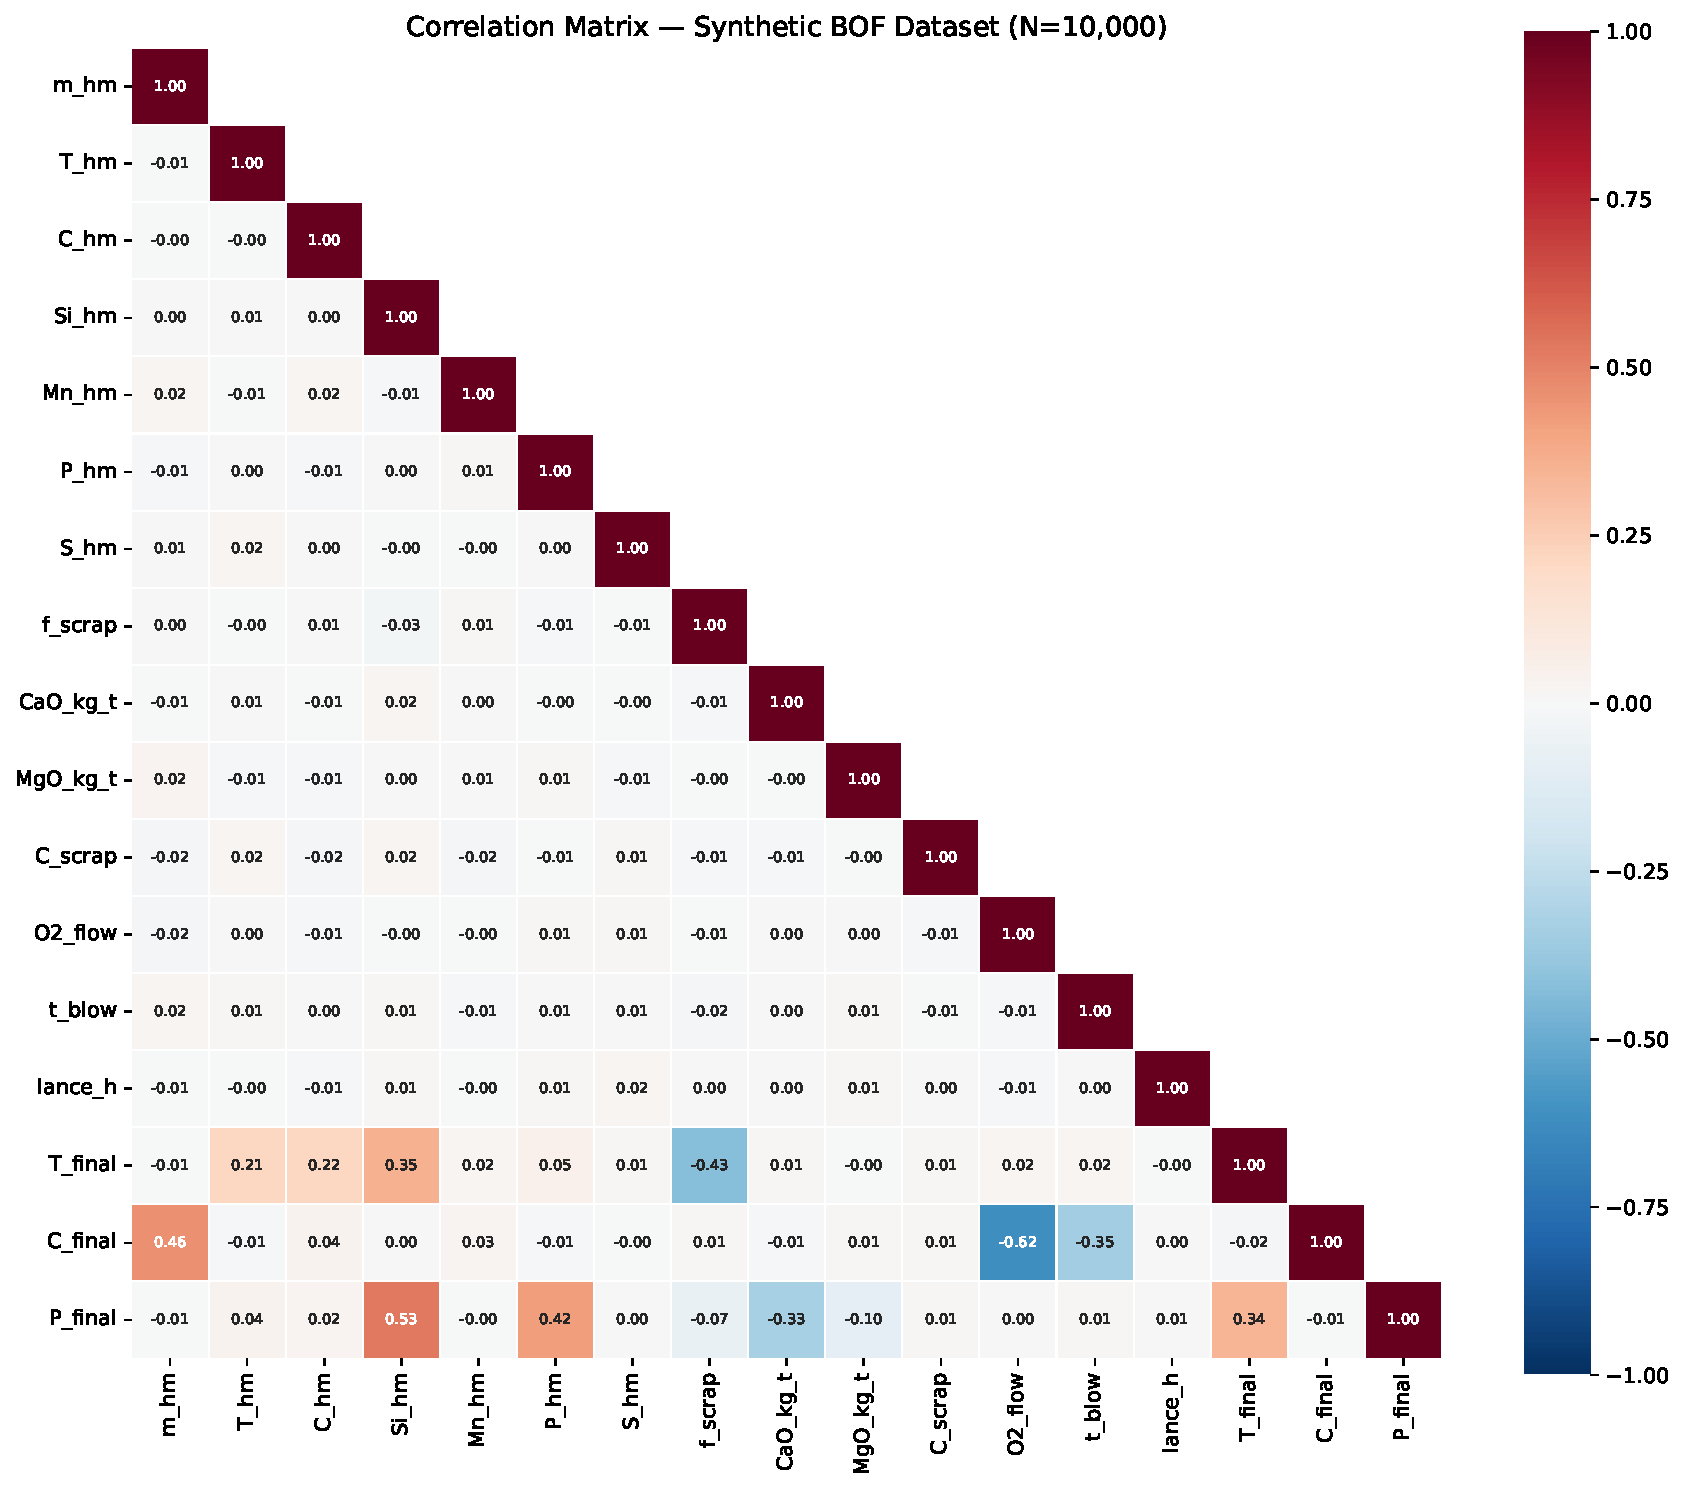
\includegraphics[width=0.82\textwidth]{Images/results/correlation_matrix.pdf}
\caption{Matriz de correlação (Pearson) do dataset sintético ($N = 10{.}000$): 14 variáveis de entrada e três alvos. As correlações mais fortes são fisicamente coerentes: $r(\texttt{O2\_flow}, [\text{C}]_\text{final}) = -0{,}62$ (mais O$_2$ remove mais C) e $r(\texttt{Si\_hm}, [\text{P}]_\text{final}) = +0{,}52$ (Si compete com P pela oxidação).}
\label{fig:corr_matrix}
\end{figure}

Os gráficos de dispersão predito vs.\ observado (Figuras~\ref{fig:predvsactual_C_cfinal} e \ref{fig:predvsactual_C_pfinal}) mostram a relação global entre predição e valor real; os gráficos de resíduo vs.\ predito (Figuras~\ref{fig:residuals_C_cfinal} e \ref{fig:residuals_C_pfinal}) são o diagnóstico apropriado para viés sistemático e heterocedasticidade, e complementam --- não substituem --- a leitura anterior. O CatBoost/Config~C para $[\text{C}]_\text{final}$ tem resíduo médio $\approx 0{,}0007\,\%$ (desprezível frente ao MAE de 0{,}0086\,\%) e correlação entre $|\text{resíduo}|$ e valor predito de apenas $0{,}017$, sem heterocedasticidade apreciável; o mesmo modelo para $[\text{P}]_\text{final}$ tem resíduo médio $\approx -0{,}0001\,\%$, mas correlação de $0{,}17$, indicando heterocedasticidade leve (erro absoluto maior para predições mais altas). Como no caso de $T_\text{final}$ (Seção~\ref{sec:resultados-A}), parte do $R^2$ de $[\text{C}]_\text{final}$ também é inflada pela censura nos limites da faixa-alvo: excluindo as amostras saturadas no conjunto de teste ($33{,}3\,\%$; a fração no dataset completo é $35{,}2\,\%$, Capítulo~\ref{chp:capitulo4}), o $R^2$ do CatBoost cai de $0{,}843$ para $0{,}766$, e o MAE sobe de $0{,}0086\,\%$ para $0{,}0101\,\%$ --- ainda um resultado sólido, mas a métrica sobre a amostra completa é, nesse caso, otimista tanto em $R^2$ quanto em MAE.

\begin{figure}[H]
\centering
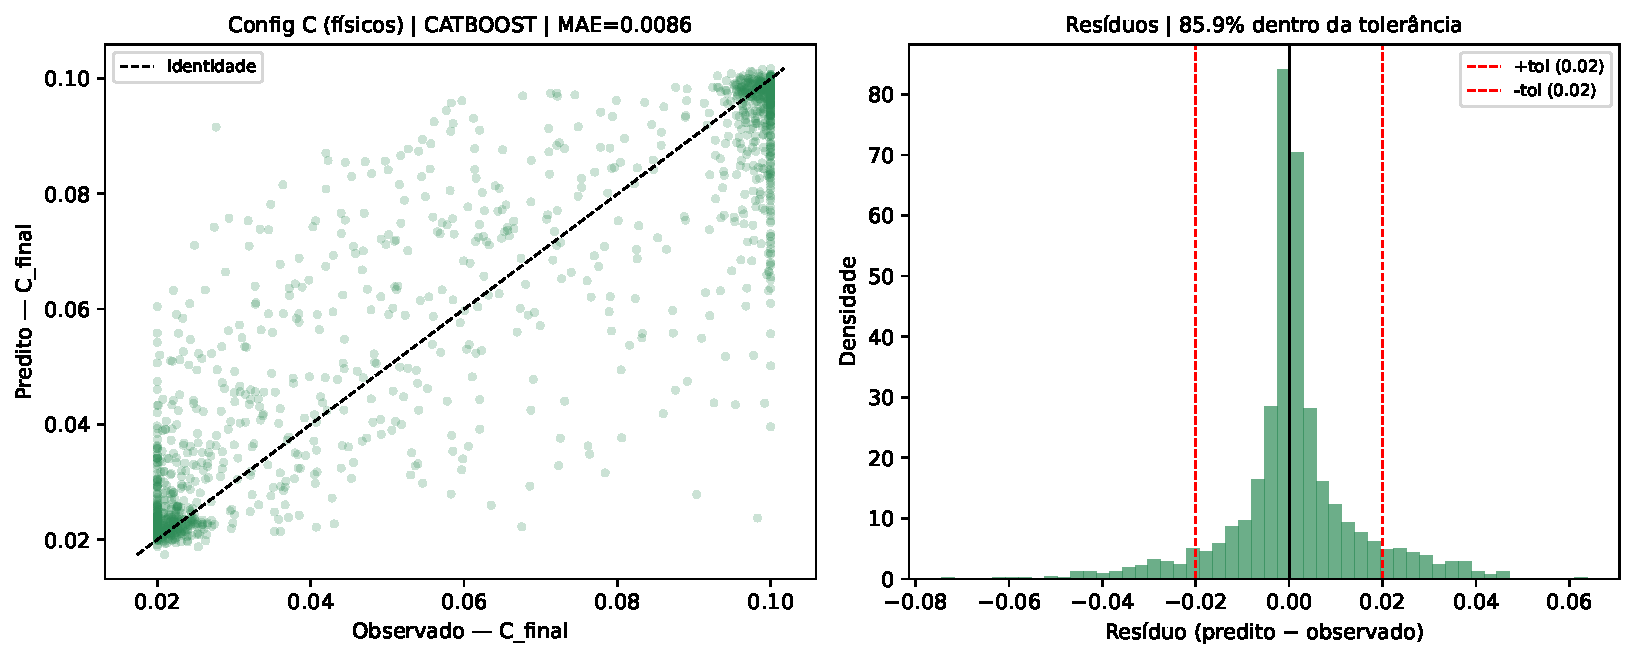
\includegraphics[width=0.75\textwidth]{Images/results/predvsactual_C_physics_catboost_C_final.pdf}
\caption{Predito vs.\ observado: CatBoost, Config~C, $[\text{C}]_\text{final}$. MAE = 0{,}0086\,\%, $R^2 = 0{,}843$.}
\label{fig:predvsactual_C_cfinal}
\end{figure}

\begin{figure}[H]
\centering
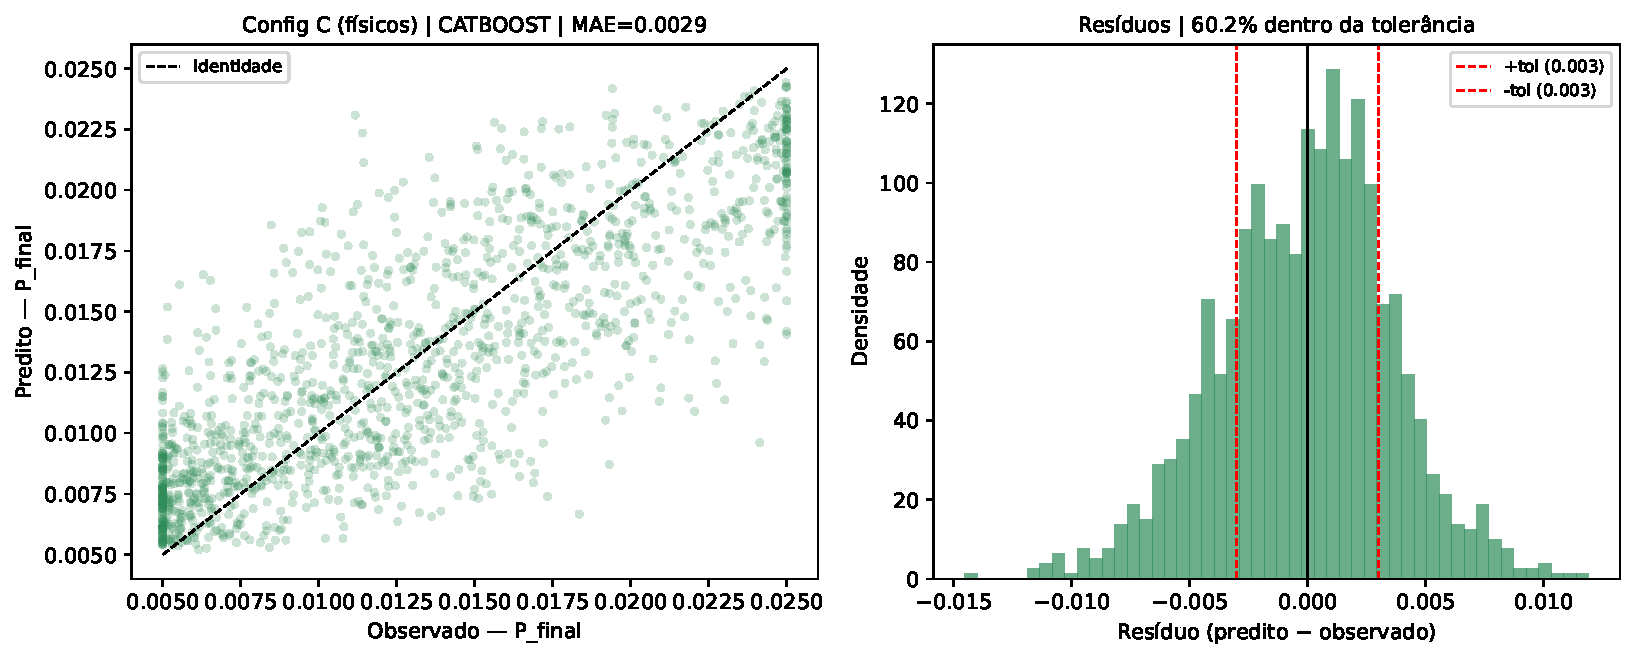
\includegraphics[width=0.75\textwidth]{Images/results/predvsactual_C_physics_catboost_P_final.pdf}
\caption{Predito vs.\ observado: CatBoost, Config~C, $[\text{P}]_\text{final}$. MAE = 0{,}0029\,\%, $R^2 = 0{,}664$.}
\label{fig:predvsactual_C_pfinal}
\end{figure}

\begin{figure}[H]
\centering
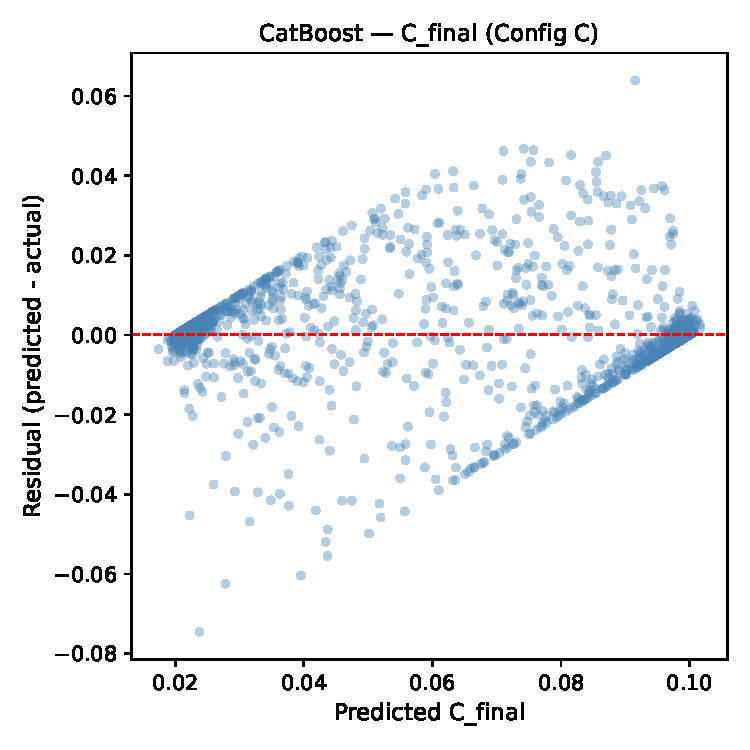
\includegraphics[width=0.75\textwidth]{Images/results/residuals_catboost_C_final.pdf}
\caption{Resíduo (predito $-$ observado) vs.\ predito: CatBoost, Config~C, $[\text{C}]_\text{final}$. Resíduo médio $\approx 0{,}0007\,\%$ (desprezível frente ao MAE de 0{,}0086\,\%) e correlação entre $|\text{resíduo}|$ e valor predito de apenas $0{,}017$: sem viés sistemático nem heterocedasticidade apreciável.}
\label{fig:residuals_C_cfinal}
\end{figure}

\begin{figure}[H]
\centering
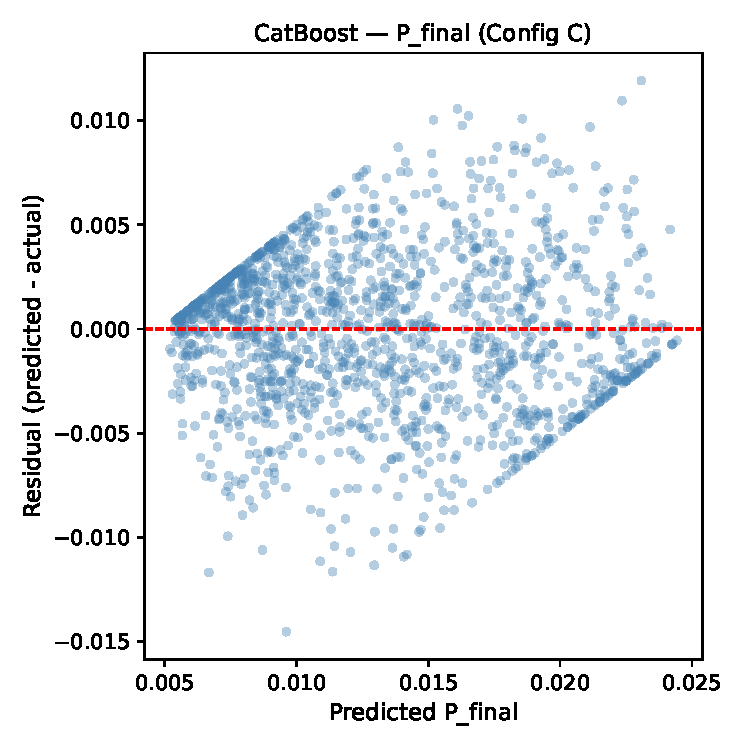
\includegraphics[width=0.75\textwidth]{Images/results/residuals_catboost_P_final.pdf}
\caption{Resíduo (predito $-$ observado) vs.\ predito: CatBoost, Config~C, $[\text{P}]_\text{final}$. Resíduo médio $\approx -0{,}0001\,\%$ (sem viés sistemático), mas correlação entre $|\text{resíduo}|$ e valor predito de $0{,}17$ --- heterocedasticidade leve, com erro absoluto ligeiramente maior para predições de $[\text{P}]_\text{final}$ mais altas.}
\label{fig:residuals_C_pfinal}
\end{figure}


\section{Análise de Interpretabilidade via SHAP}
\label{sec:shap-resultados}

A análise SHAP (SHapley Additive exPlanations) foi conduzida sobre três modelos representativos de famílias distintas da Config~C (RF, XGBoost, MLP --- ensemble de bagging, \textit{boosting} e rede neural, respectivamente) para cada alvo, utilizando TreeExplainer para os modelos de árvore e KernelExplainer com 200 amostras de fundo para o MLP\,\cite{lundberg2017unified,manojlovic2022eaf,xia2024dmpinn}. Esses três não são necessariamente os de menor MAE em cada alvo individualmente (Tabelas~\ref{tbl:resultados_configA}--\ref{tbl:resultados_configC}) --- notavelmente, o MLP é o pior modelo da Config~C para $T_\text{final}$ --- mas cobrem os principais paradigmas de modelo usados na comparação, o que é relevante para a leitura das hipóteses H1, H4 e H5 adiante, cuja média entre os três é por vezes dominada pelo modelo com maior magnitude de SHAP bruto, não pelo de melhor desempenho preditivo. A Tabela~\ref{tbl:shap_importance} apresenta as cinco features de maior importância média $|\text{SHAP}|$ por alvo, consolidadas como média aritmética dos três modelos.

\begin{table}[H]
\caption{Top-5 features por importância SHAP média $\overline{|\phi|}$ (média de RF, XGBoost, MLP da Config~C). Features físico-derivadas são marcadas com $\bullet$.}
\label{tbl:shap_importance}
\centering
\footnotesize
\setlength{\tabcolsep}{4pt}
\begin{tabular}{clrclrclr}
\hline
\multicolumn{3}{c}{$T_\text{final}$} & \multicolumn{3}{c}{$[\text{C}]_\text{final}$} & \multicolumn{3}{c}{$[\text{P}]_\text{final}$} \\
\cline{1-3}\cline{4-6}\cline{7-9}
\# & Feature & $\overline{|\phi|}$ & \# & Feature & $\overline{|\phi|}$ & \# & Feature & $\overline{|\phi|}$ \\
\hline
1 & \texttt{t\_blow}              & 87,07 & 1 & $\bullet$ \texttt{o2\_efficiency}  & 0,0195 & 1 & $\bullet$ \texttt{slag\_basicity} & 0,00282 \\
2 & $\bullet$ \texttt{o2\_efficiency}      & 73,69 & 2 & \texttt{O2\_flow}               & 0,0069 & 2 & \texttt{P\_hm}                   & 0,00228 \\
3 & $\bullet$ \texttt{decarb\_rate}        & 67,10 & 3 & $\bullet$ \texttt{fe\_oxidation\_loss}   & 0,0036 & 3 & $\bullet$ \texttt{theo\_o2\_demand}        & 0,00077 \\
4 & $\bullet$ \texttt{slag\_basicity}      & 51,91 & 4 & \texttt{t\_blow}                & 0,0027 & 4 & \texttt{Si\_hm}                  & 0,00062 \\
5 & \texttt{O2\_flow}            & 41,87 & 5 & \texttt{m\_hm}                  & 0,0023 & 5 & \texttt{m\_hm}                   & 0,00050 \\
\hline
\end{tabular}
\end{table}

A Tabela~\ref{tbl:shap_importance} mostra que features físico-derivadas ocupam posições relevantes para os três alvos: \texttt{o2\_efficiency} e \texttt{decarb\_rate} são as features \#2 e \#3 para $T_\text{final}$ (com a ressalva sobre agregação entre modelos discutida adiante); \texttt{o2\_efficiency} é a feature \#1 para $[\text{C}]_\text{final}$ no RF e no XGBoost, e \#2 no MLP (atrás de \texttt{O2\_flow}); e \texttt{slag\_basicity} é a feature \#1 para $[\text{P}]_\text{final}$, embora com margem modesta sobre a segunda posição --- indicando que a composição bruta do gusa continua sendo um preditor quase tão relevante quanto o atributo físico-derivado combinado. A Figura~\ref{fig:shap_beeswarm_cfinal} mostra o gráfico \textit{beeswarm} do XGBoost para $[\text{C}]_\text{final}$, confirmando que \texttt{o2\_efficiency} domina a predição com relação monotônica \emph{direta} --- maior \texttt{o2\_efficiency} corresponde a maior $[\text{C}]_\text{final}$ predito (SHAP médio assinado positivo nos três modelos), não o inverso: como \texttt{o2\_efficiency} = \texttt{theo\_o2\_demand} / (O$_2$\_soprado $\times$ tempo de sopro) e \texttt{theo\_o2\_demand} cresce com a carga inicial de impurezas do gusa, corridas com maior carga inicial produzem simultaneamente maior \texttt{o2\_efficiency} \emph{e} maior $[\text{C}]_\text{final}$ residual --- uma relação de causa comum, não de causalidade direta entre o atributo e o alvo.

\begin{figure}[H]
\centering
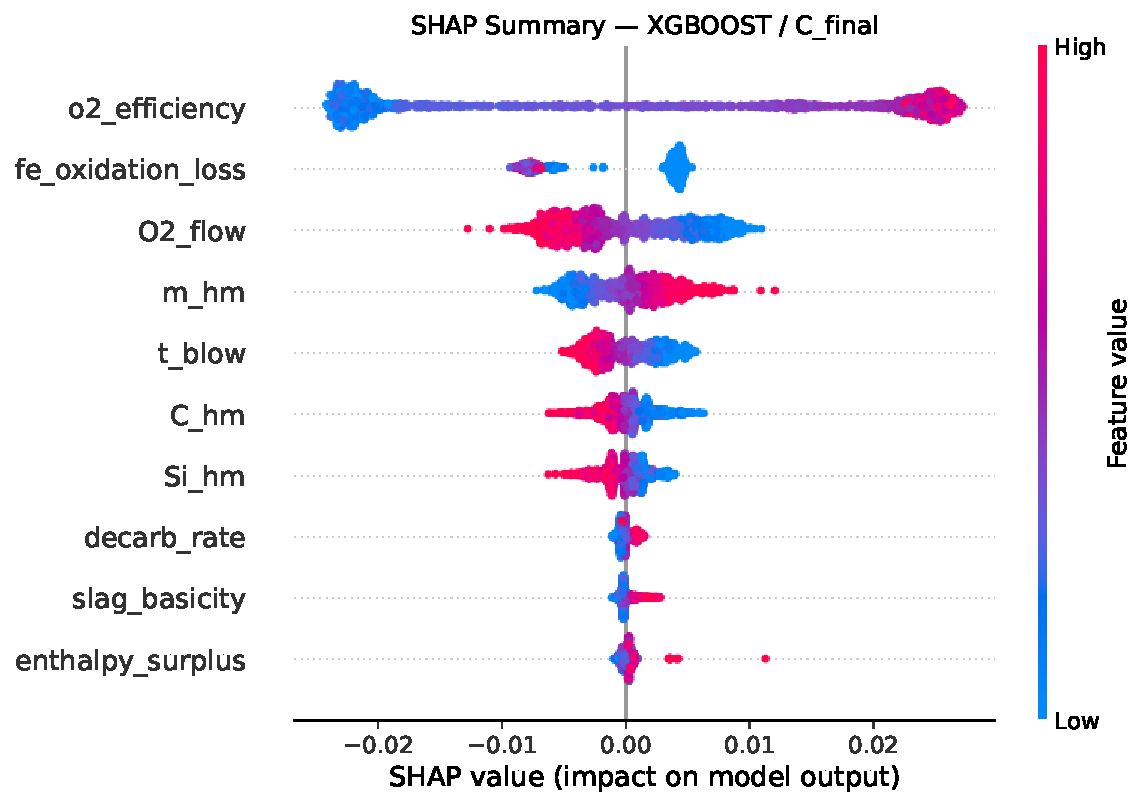
\includegraphics[width=0.85\textwidth]{Images/shap/summary_xgboost_C_final.pdf}
\caption{Gráfico \textit{beeswarm} SHAP do XGBoost (Config~C) para $[\text{C}]_\text{final}$. A feature \texttt{o2\_efficiency} (físico-derivada) domina, com importância $3{,}8\times$ superior à segunda posição neste modelo (\texttt{fe\_oxidation\_loss}); a relação é direta, não inversa (ver texto).}
\label{fig:shap_beeswarm_cfinal}
\end{figure}

\begin{figure}[H]
\centering
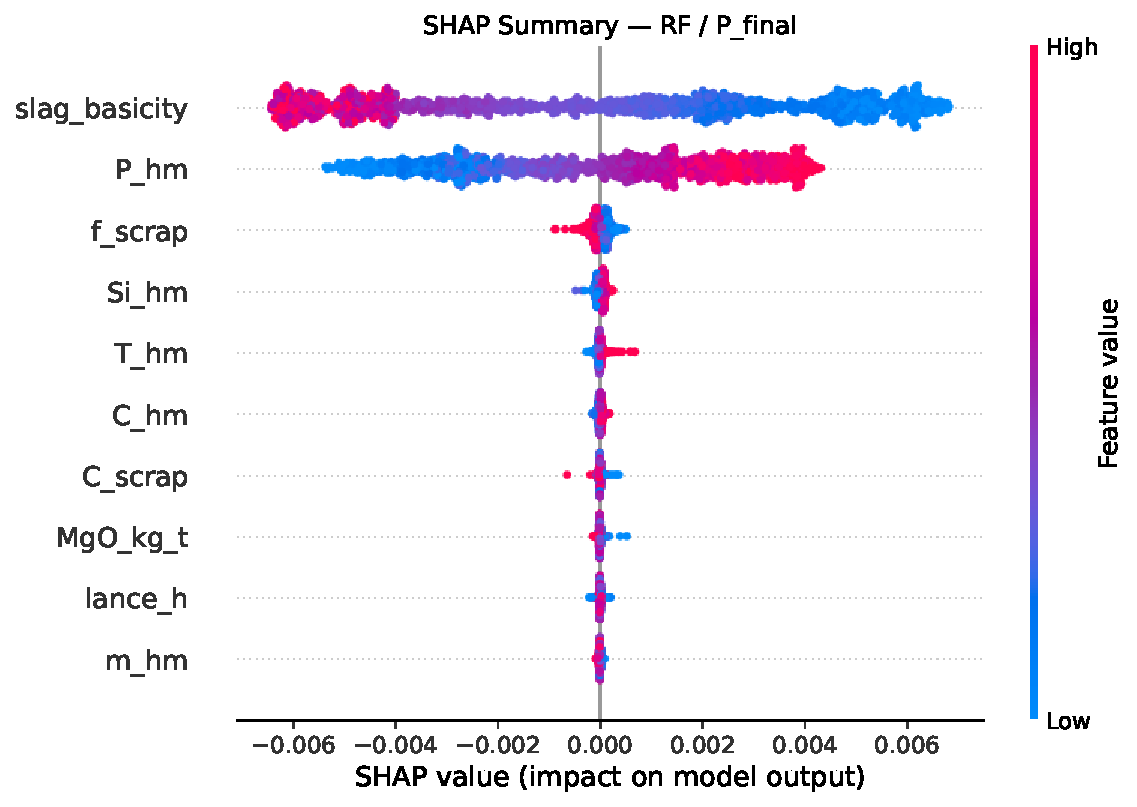
\includegraphics[width=0.85\textwidth]{Images/shap/summary_rf_P_final.pdf}
\caption{Gráfico \textit{beeswarm} SHAP do RF (Config~C) para $[\text{P}]_\text{final}$. \texttt{slag\_basicity} (físico-derivada) é a feature de maior importância, com margem modesta ($1{,}63\times$ neste modelo) sobre \texttt{P\_hm}, consistente com o mecanismo termodinâmico de desfosforação pela basicidade da escória~\cite{bae2020bof}.}
\label{fig:shap_beeswarm_pfinal}
\end{figure}

A Tabela~\ref{tbl:shap_hypotheses} reporta os resultados dos cinco testes de coerência física definidos no Capítulo~\ref{chp:capitulo4} (H1 e H2 aceitam \texttt{theo\_o2\_demand} \emph{ou} \texttt{o2\_efficiency} como satisfazendo a hipótese, conforme formulado no Capítulo~\ref{chp:capitulo1}; H4 e H5 são resolvidas pelo sinal médio do SHAP, não apenas por sua magnitude).

\begin{table}[H]
\caption{Resultados dos testes de hipótese de coerência física SHAP (H1--H5).}
\label{tbl:shap_hypotheses}
\centering
\footnotesize
\resizebox{\textwidth}{!}{%
\setlength{\tabcolsep}{4pt}
\begin{tabular}{cp{4.2cm}p{1.8cm}p{6.0cm}}
\hline
\textbf{H} & \textbf{Hipótese} & \textbf{Resultado} & \textbf{Evidência} \\
\hline
H1 & \texttt{theo\_o2\_demand} ou \texttt{o2\_efficiency} top-3 para $T_\text{final}$ & Confirmada na média, não por modelo individual & Top-3 médio: \texttt{t\_blow}, \texttt{o2\_efficiency}, \texttt{decarb\_rate}; mas apenas no MLP (2\textordmasculine) --- RF e XGBoost não incluem nenhum atributo de O$_2$ em seus próprios top-3 \\[3pt]
H2 & \texttt{theo\_o2\_demand} ou \texttt{o2\_efficiency} top-3 para $[\text{C}]_\text{final}$ & Confirmada por modelo individual & Top-3: \texttt{o2\_efficiency}, \texttt{O2\_flow}, \texttt{fe\_oxidation\_loss}; \texttt{o2\_efficiency} está no top-3 dos três modelos (\#1 em RF/XGBoost, \#2 no MLP) \\[3pt]
H3 & \texttt{slag\_basicity} top-3 para $[\text{P}]_\text{final}$ & Confirmada & \texttt{slag\_basicity} é \#1, mas com margem modesta sobre \texttt{P\_hm} \\[3pt]
H4 & \texttt{decarb\_rate} dir.\ negativa para $[\text{C}]_\text{final}$ & Confirmada na média, sinal divergente entre modelos & SHAP médio assinado $= -0{,}000114$; sinal positivo (oposto ao hipotetizado) no RF, negativo no XGBoost e no MLP (dominante na média) \\[3pt]
H5 & \texttt{enthalpy\_surplus} dir.\ positiva para $T_\text{final}$ & Refutada na média, sinal divergente entre modelos & SHAP médio assinado $= -1{,}45$; sinal positivo (hipotetizado) em RF e XGBoost, negativo e de magnitude dominante no MLP \\
\hline
\end{tabular}}
\end{table}

H2 é confirmada de forma robusta: \texttt{o2\_efficiency} = \texttt{theo\_o2\_demand} / (O$_2$\_soprado $\times$ tempo de sopro) está no top-3 para $[\text{C}]_\text{final}$ nos três modelos individualmente (\#1 no RF e no XGBoost, \#2 no MLP, atrás de \texttt{O2\_flow}), não apenas na média. H1 é confirmada apenas pelo critério pré-registrado de média entre modelos --- \texttt{o2\_efficiency} é a \#2 no top-3 médio para $T_\text{final}$ --- mas essa média é dominada pelo MLP: individualmente, RF e XGBoost não colocam nenhum atributo relacionado a O$_2$ em seus próprios top-3 para $T_\text{final}$ (Seção~\ref{sec:shap-resultados} discute por que agregar $|\phi|$ entre TreeExplainer e KernelExplainer sem normalização favorece o modelo de escala bruta maior). H1 deve, portanto, ser lida como confirmada pelo protocolo pré-registrado, mas frágil a essa escolha de agregação --- o mesmo problema metodológico identificado adiante para H4 e H5. Onde \texttt{o2\_efficiency} de fato domina (H2), a relação com o alvo é direta, não inversa: como discutido acima, ambos crescem juntos com a carga inicial de impurezas do gusa~\cite{chattopadhyay2022hybrid}.

H3 é confirmada: \texttt{slag\_basicity} é a feature de maior importância para $[\text{P}]_\text{final}$ --- o critério pré-registrado (top-3) é satisfeito com folga --- ainda que por margem modesta sobre \texttt{P\_hm} (o teor bruto de fósforo do gusa); isso é fisicamente sensato, já que o teor inicial de P é, por si só, um forte preditor de quanto restará após a remoção parcial\,\cite{bae2020bof,chattopadhyay2022hybrid}, e não contradiz a hipótese, que nunca postulou magnitude de dominância, apenas posição relativa.

H4 é confirmada apenas na média, com o mesmo padrão de fragilidade identificado para H1 e H5: o sinal assinado de \texttt{decarb\_rate} para $[\text{C}]_\text{final}$ é positivo no RF (o oposto do hipotetizado), negativo no XGBoost e fortemente negativo no MLP, que domina a média. A relação algébrica esperada é, de fato, ambígua a priori: $\texttt{decarb\_rate} = [\text{C}]_\text{hm} / t_\text{blow}$ e $[\text{C}]_\text{final} \propto [\text{C}]_\text{hm} \cdot \exp(-k \cdot r_{\text{O}_2})$ (Capítulo~\ref{chp:capitulo4}) --- um $[\text{C}]_\text{hm}$ maior eleva ambos simultaneamente (sinal positivo, como no RF), enquanto um $t_\text{blow}$ maior reduz \texttt{decarb\_rate} mas também prolonga a oxidação, reduzindo $[\text{C}]_\text{final}$ (sinal negativo, como no XGBoost e no MLP). Qual mecanismo domina depende de qual dos dois canais cada modelo pondera mais fortemente, não de uma direção termodinâmica única e inequívoca; a leitura mais honesta é que H4 captura uma associação estatística real, mas de direção dependente do modelo, e não uma relação causal de sinal único.

H5 é refutada na média dos três modelos, mas o resultado por modelo é menos unânime do que a média sugere: o SHAP médio assinado de \texttt{enthalpy\_surplus} para $T_\text{final}$ é positivo --- o sinal hipotetizado --- tanto no RF ($+0{,}032$) quanto no XGBoost ($+0{,}041$), e apenas o MLP mostra sinal negativo ($-4{,}43$); como o MLP usa KernelExplainer (valores aproximados sobre 200 amostras de fundo) em vez do TreeExplainer exato dos outros dois, e sua magnitude é de 1 a 2 ordens de grandeza maior nesta feature (comparado a $|\phi| = 0{,}22$ no RF e $0{,}71$ no XGBoost), a média simples de três modelos é dominada por um único valor de magnitude e método de cálculo distintos. Em qualquer leitura, \texttt{enthalpy\_surplus} tem importância baixa para $T_\text{final}$ (13\textordmasculine\ de 22 atributos por $|\phi|$ médio, Seção~\ref{sec:shap-resultados}), de modo que H5 --- confirmada ou refutada --- não afeta a conclusão central de que $T_\text{final}$ permanece dominado por variância irredutível não capturada por nenhum atributo disponível. Uma explicação plausível para o sinal negativo específico do MLP é a de que \texttt{enthalpy\_surplus} é calculado com constantes fixas e frações de oxidação teóricas completas (Nível~2, §\,\ref{subsec:ameacas-validade}), enquanto $T_\text{final}$ é gerado com eficiência térmica e frações de remoção específicas à corrida ($\eta_\text{eff}$, Nível~1); esta é uma leitura pós-hoc, não uma hipótese testada de forma independente, e fica registrada como direção de investigação futura em vez de explicação definitiva.

Em síntese, a análise SHAP é consistente com os modelos da Config~C utilizando os atributos físico-derivados como vetores relevantes de predição, com quatro das cinco hipóteses de coerência física não falsificadas; a exceção (H5) mostra sinal dependente do modelo (positivo em RF e XGBoost, negativo e dominante no MLP) sobre um atributo de importância já baixa para $T_\text{final}$, o que por si só é um resultado informativo sobre os limites de agregar SHAP entre modelos com métodos de explicação distintos.


\section{Comparação com a Literatura}
\label{sec:comparacao-literatura}

Os ganhos observados na Config~C podem ser contextualizados frente aos resultados reportados na literatura de predição de ponto final BOF, reconhecendo que diferenças em dados (sintéticos vs.\ industriais), escalas de planta e variáveis de entrada tornam a comparação qualitativa e não direta.

\citeonline{bae2020bof} reportam que a adição de 17 atributos termodinâmicos a uma rede neural para predição de $T_\text{final}$ em dados reais de planta eleva a taxa de acerto dentro de $\pm 10\,^\circ\text{C}$ em 2--4 pontos percentuais (os autores não reportam um MAE absoluto de referência). Nesta dissertação, o ganho em $w_\text{tol}$ da Config~C sobre a Config~A para $T_\text{final}$ é nulo ou levemente negativo (o melhor modelo pareado, SVR, cai de $35{,}9\,\%$ para $34{,}5\,\%$). A diferença crucial é que \citeonline{bae2020bof} incluem medições de sublança intermediárias como atributos, enquanto esta dissertação restringe-se a variáveis pré-sopro --- um cenário informacionalmente mais restritivo. Como referência de MAE absoluto no mesmo regime pré-sopro (sem off-gas), \citeonline{zhou2024bof} reportam $7{,}96\,^\circ\text{C}$ (LightGBM, 45 variáveis tabulares) --- inferior aos $21{,}86$--$27{,}37\,^\circ\text{C}$ desta dissertação, refletindo o benefício de dados reais de planta e um conjunto de atributos tabulares mais amplo.

Para $[\text{C}]_\text{final}$, \citeonline{zhou2024bof} reportam MAE de $6{,}92\times10^{-3}\,\%$ com CatBoost sobre dados reais de planta, também no regime tabular sem off-gas (o modelo combinado com off-gas dos mesmos autores reduz esse valor a $6{,}41\times10^{-3}\,\%$ em teste, mas usa informação temporal indisponível nesta dissertação). O melhor resultado da Config~C (CatBoost, MAE~$= 0{,}0086\,\%$) é cerca de $24\,\%$ maior --- ou seja, pior --- que o valor tabular de \citeonline{zhou2024bof}, mesmo com o alvo desta dissertação já se beneficiando de uma proporção maior de amostras saturadas na faixa (\S\,\ref{sec:diagnostico-visual}). A diferença é plausivelmente explicada tanto pelo conjunto de atributos tabulares mais amplo de \citeonline{zhou2024bof} ($45$ variáveis, contra $22$ nesta dissertação) quanto pelo fato de que os alvos provêm de distribuições distintas --- uma gerada por um modelo físico simplificado sem os modos de falha, ruído de processo e não-linearidades de uma planta real, a outra medida diretamente em operação --- de modo que a proximidade ou distância numérica entre os MAE não deve ser lida como evidência de equivalência ou inferioridade metodológica entre as abordagens~\cite{shao2024hybrid}.

Para $[\text{P}]_\text{final}$, \citeonline{chattopadhyay2022hybrid} reportam que modelos híbridos serial (físico + ML) atingem MAE $\approx 0{,}004\,\%$ em dados reais, e a Config~C obtém 0{,}0029\,\% com CatBoost --- valor numericamente menor, mas obtido sobre dados sintéticos sem a complexidade total de uma planta real, o que impede tratar a comparação como evidência de superioridade\,\cite{buggineni2024synthetic}. A Tabela~\ref{tbl:comparacao_literatura} consolida essa comparação.

\begin{table}[H]
\caption{Contextualização do MAE desta dissertação frente à literatura. $\dagger$: dados sintéticos; demais: dados industriais reais. Os valores \textbf{não são diretamente comparáveis}: diferenças em escala de planta, variáveis disponíveis e, sobretudo, na natureza dos dados (sintéticos vs.\ reais) impedem inferir superioridade ou equivalência a partir da proximidade numérica.}
\label{tbl:comparacao_literatura}
\centering
\footnotesize
\setlength{\tabcolsep}{4pt}
\begin{tabular}{llrrp{3.8cm}}
\hline
\textbf{Alvo} & \textbf{Estudo} & \textbf{MAE} & \textbf{Modelo} & \textbf{Observação} \\
\hline
$T_\text{final}$ (°C) & \citeonline{zhou2024bof} & 7,96 & LightGBM & 45 var.\ tabulares, dados reais \\
 & Esta dissert.$^\dagger$ & 21,86 & SVR (A) & Apenas variáveis pré-sopro \\
\hline
$[\text{C}]$ (\%) & \citeonline{zhou2024bof} & 0,00692 & CatBoost & 45 var.\ tabulares, dados reais \\
 & Esta dissert.$^\dagger$ & 0,0086 & CatBoost (C) & 8 features físicas estáticas \\
\hline
$[\text{P}]$ (\%) & \citeonline{chattopadhyay2022hybrid} & $\approx$0,004 & Híbrido & Serial (físico+ML), dados reais \\
 & Esta dissert.$^\dagger$ & 0,0029 & CatBoost (C) & 8 features físicas estáticas \\
\hline
\end{tabular}
\end{table}

A engenharia de atributos físico-derivados produz, em suma, ganhos estatisticamente significativos e de relevância prática para $[\text{C}]_\text{final}$ (10 dos 11 modelos) e para $[\text{P}]_\text{final}$ (8 dos 11 modelos, com seis passando a atender ao limiar industrial contra apenas um na linha de base), mas não resolve o gargalo estrutural de $T_\text{final}$, cujo erro é dominado por variância irredutível do processo e pela ausência de informação temporal. O teste de extrapolação, além disso, mostra que esses ganhos para $[\text{C}]_\text{final}$ e $[\text{P}]_\text{final}$ se mantêm --- e no caso do fósforo, permanecem dentro do limiar industrial --- sob a extensão moderada de faixa de amostragem testada. A hipótese central da dissertação é, portanto, parcialmente confirmada: os atributos físico-derivados melhoram a predição frente à linha de base nos dois alvos com relação física mais direta com as features propostas, e esse benefício não desaparece sob a extrapolação testada, mas depende do alvo, da família de modelo utilizada e da informação disponível no momento da predição.

Toda essa avaliação, cabe reiterar, ocorre sobre dados sintéticos gerados por um modelo físico simplificado, não sobre uma planta real (Capítulo~\ref{chp:con}, Seção~\ref{sec:limitacoes}); os ganhos relativos entre configurações são internos ao universo do gerador e quantificam o valor da engenharia de atributos dentro dele, não necessariamente a magnitude que se observaria em dados industriais reais. A validação com dados de planta permanece, portanto, condição necessária antes de qualquer inferência sobre aplicabilidade operacional.

\chapter{Considerações Finais}
\label{chp:con}

\section{Síntese do Trabalho}
\label{sec:sintese}

Esta dissertação investigou a hipótese central de que a incorporação de conhecimento físico-químico diretamente na engenharia de atributos --- em vez de restringi-lo às funções de perda ou às arquiteturas de rede --- produz modelos de regressão supervisionada mais acurados, mais robustos e mais interpretáveis para a predição de parâmetros de fim de corrida em Fornos Básicos a Oxigênio (BOF). A motivação partiu de um diagnóstico conhecido na literatura: modelos puramente orientados a dados tendem a apresentar degradação significativa de desempenho quando aplicados a regiões operacionais fora da distribuição de treino, especialmente em processos siderúrgicos com dados escassos e ruidosos \cite{bae2020bof,willard2020integrating}.

A resposta metodológica proposta organiza-se em quatro etapas sequenciais. Primeiro, um conjunto de dados sintéticos de BOF foi gerado via simulação de Monte Carlo, com N=10.000 corridas fisicamente válidas, impondo restrições de balanço entálpico e estequiométrico às amostras \cite{buggineni2024synthetic,melo2024synthetic}. Segundo, os dados brutos foram expandidos com oito atributos físico-derivados --- demanda teórica de oxigênio, eficiência de sopro, entalpia acumulada, fração de massa oxidada, taxa de descarbonetação, basicidade da escória, capacidade de fusão da sucata e perda de ferro --- todos calculados a partir das equações de balanço descritas no Capítulo~\ref{chp:capitulo4}. Terceiro, três configurações experimentais foram definidas: Config~A (baseline, atributos brutos, conjunto completo de modelos otimizados via Optuna), Config~B (aprendizado profundo, atributos brutos, MLP com busca de arquitetura via Optuna) e Config~C (física informada, atributos brutos mais os oito físico-derivados, conjunto completo de modelos). Quarto, os modelos foram avaliados por MAE, RMSE e $R^2$ para três variáveis-alvo: temperatura final ($T_{\text{final}}$), teor de carbono final ($[\text{C}]_{\text{final}}$) e teor de fósforo final ($[\text{P}]_{\text{final}}$), adotando as tolerâncias industriais de $\text{MAE} \leq 10\,^\circ\text{C}$, $\text{MAE} \leq 0{,}020\,\%$ e $\text{MAE} \leq 0{,}003\,\%$, respectivamente, como critério de aprovação \cite{zhou2024bof,bae2020bof}.

A hipótese central foi parcialmente confirmada: os atributos físico-derivados produziram ganhos estatisticamente significativos para $[\text{C}]_\text{final}$ (10/11 modelos melhoram, $p < 0{,}05$) e $[\text{P}]_\text{final}$ (8/11 modelos melhoram), com seis modelos de $[\text{P}]_\text{final}$ passando a atender ao limiar industrial de $0{,}003\,\%$ contra apenas um na linha de base, mas não resolveram o gargalo estrutural de $T_\text{final}$ (nenhum modelo melhora significativamente), cujo erro é dominado por variância irredutível associada a grandezas estocásticas não observáveis ($\eta_\text{eff}$). O teste de extrapolação mostra que esses ganhos em $[\text{C}]_\text{final}$ e $[\text{P}]_\text{final}$ se mantêm sob perturbação moderada fora da faixa de calibração. A análise SHAP é consistente, em grande parte, com a relevância física esperada dos atributos: \texttt{o2\_efficiency} é a feature de maior importância para $[\text{C}]_\text{final}$ nos três modelos testados individualmente, e \texttt{slag\_basicity} para $[\text{P}]_\text{final}$ (embora com margem modesta sobre o teor bruto de fósforo do gusa) --- sem que isso prove, por si só, captura causal de estrutura física\,\cite{manojlovic2022eaf,xia2024dmpinn}.


\section{Principais Contribuições}
\label{sec:contribuicoes}

O trabalho entrega quatro contribuições concretas à interseção entre aprendizado de máquina e modelagem de processos siderúrgicos:

\textbf{C1 — Dataset sintético de BOF com validação física.} Um conjunto de 10.000 corridas sintéticas de BOF, amostrado dentro de faixas operacionais documentadas na literatura \cite{chattopadhyay2022hybrid,bae2020bof} e validado por consistência termodinâmica (erro de balanço entálpico $< 10\%$). O dataset supre a carência crítica de dados industriais abertos para pesquisa em predição de fim de corrida BOF, problema amplamente reconhecido na área \cite{ghalati2023review,zhou2024bof}. O código de geração e as constantes físicas utilizadas são disponibilizados integralmente no repositório do projeto\footnote{\url{https://github.com/devGvieira/bof-piml-dissertation}}, permitindo reprodução e extensão a outras faixas operacionais.

\textbf{C2 — Conjunto padronizado de oito atributos físico-derivados para BOF.} A sistematização das oito features calculadas a partir de balanços de massa e energia --- com equações, constantes termodinâmicas e referências bibliográficas explícitas para cada uma --- oferece um ponto de partida reproduzível para estudos futuros de engenharia de atributos em processos de refino. Ao contrário de abordagens que integram a física à função de perda \cite{raissi2019pinns,xia2024dmpinn}, a estratégia adotada é agnóstica em relação ao algoritmo de aprendizado e pode ser aplicada a qualquer modelo de regressão supervisionada.

\textbf{C3 — Comparação sistemática de três configurações experimentais em onze modelos e três variáveis-alvo.} O protocolo A×B×C isola dois fatores independentes: o ganho proveniente de atributos físicos (A×C) e o ganho proveniente de profundidade arquitetural (A×B), além de avaliar sua interação (B×C). Com 11 modelos (Ridge, Lasso, ElasticNet, SVR, KNN, RF, GBM, XGBoost, LightGBM, CatBoost, MLP) avaliados em três alvos, o experimento gera evidência quantitativa sobre qual fator --- física ou capacidade de representação --- contribui mais para a qualidade preditiva no domínio BOF. Protocolos similares de comparação sistemática em contextos siderúrgicos são escassos na literatura \cite{ghalati2023review,shao2024hybrid}.

\textbf{C4 — Análise SHAP com validação de consistência física.} A análise SHAP (SHapley Additive exPlanations) é aplicada não apenas como ferramenta de ranqueamento de importância de atributos, mas como mecanismo de validação qualitativa, sob um protocolo de falsificação pré-registrado (Capítulo~\ref{chp:capitulo1}): quatro das cinco hipóteses de coerência física testáveis (H1–H5) não foram falsificadas, o que é consistente com --- ainda que não prove --- a captura de estrutura física real pelos modelos, e não apenas de correlações espúrias \cite{manojlovic2022eaf,xia2024dmpinn}. A exceção (H5) e a fragilidade de H1 e H4 (Capítulo~\ref{chp:resultados}) revelam um limite metodológico específico: a média de importância SHAP entre modelos explicados por métodos distintos (TreeExplainer exato vs.\ KernelExplainer aproximado) pode ser dominada por um único modelo de escala bruta maior, mascarando divergência de sinal ou de posição entre os demais — um resultado negativo tratado como achado, não omitido. Esta perspectiva estende a aplicação de SHAP em siderurgia, onde seu uso é predominantemente descritivo na literatura revisada nesta dissertação \cite{ghalati2023review}.


\section{Limitações}
\label{sec:limitacoes}

A validade externa dos resultados desta pesquisa está condicionada a três limitações estruturais que devem ser consideradas na interpretação das conclusões. Ressalta-se que nenhum dado industrial proprietário foi empregado nesta pesquisa; todos os parâmetros físicos, faixas operacionais e constantes termodinâmicas derivam exclusivamente de literatura científica publicada\,\cite{cai2021heat,bae2020bof,chattopadhyay2022hybrid,xia2024dmpinn}.

Primeiramente, toda a experimentação é conduzida sobre dados sintéticos, gerados por um modelo físico simplificado que não inclui dinâmicas de escória, perfis temporais de sopro, variações de composição do sucateado ou efeitos de desgaste refratário. Comparações entre configurações AI e AI-física sobre dados sintéticos quantificam o ganho relativo da engenharia de atributos dentro do universo do modelo generativo, mas não permitem inferência direta sobre desempenho em plantas reais. A validação com dados industriais reais é, portanto, condição necessária para afirmar aplicabilidade operacional --- e permanece como trabalho futuro essencial \cite{buggineni2024synthetic,morales2025synthetic}.

Em segundo lugar, o modelo físico subjacente é estático e de estado final: prediz os valores de saída ao término da corrida a partir de variáveis de entrada iniciais, sem modelar a trajetória temporal do processo. Fenômenos como a dinâmica de formação de escória, o perfil de sopro ao longo do tempo e a evolução do banho metálico são ignorados. Modelos que incorporam perfis temporais --- como os abordados por \citeonline{shao2024hybrid} com dados de off-gas e por \citeonline{xia2024dmpinn} com PINNs dinâmicas --- podem capturar informações adicionais não disponíveis nesta formulação.

Finalmente, a generalização dos modelos treinados para plantas siderúrgicas distintas daquela que deu origem aos parâmetros físicos adotados pode exigir re-calibração das constantes, dos limites de amostragem e dos pesos do modelo físico. As tolerâncias industriais adotadas ($\text{MAE} \leq 10\,^\circ\text{C}$ para temperatura, $\leq 0{,}020\,\%$ para carbono e $\leq 0{,}003\,\%$ para fósforo) refletem condições de operação típicas documentadas na literatura \cite{zhou2024bof,bae2020bof}, mas podem diferir entre plantas com diferentes capacidades de convertedor, qualidades de sucata e fontes de ferro-gusa.


\section{Trabalhos Futuros}
\label{sec:trabalhos-futuros}

As limitações identificadas na seção anterior delineiam naturalmente as extensões mais relevantes desta pesquisa.

A prioridade imediata é a validação com dados reais de planta. A parceria com uma siderurgia nacional para acesso a históricos de corridas --- mesmo que anonimizados --- permitiria avaliar se os ganhos preditivos observados em dados sintéticos se transferem para o domínio real, e em que magnitude. A metodologia de engenharia de atributos físico-derivados é, por construção, transferível: as equações de balanço são universais, e apenas os parâmetros numéricos requerem calibração para cada instalação \cite{chattopadhyay2022hybrid,shao2024hybrid}.

Uma extensão natural do trabalho é a incorporação de perfis temporais de sopro e dados de off-gas como atributos adicionais. Estudos recentes demonstram que a composição dinâmica dos gases de exaustão (CO/CO$_2$) fornece informação contínua sobre o progresso da descarbonetação, permitindo predições mais precisas de $[\text{C}]_{\text{final}}$ \cite{zhou2024bof,shao2024hybrid}. A combinação desses sinais com os atributos físico-derivados estáticos propostos nesta dissertação configuraria um framework híbrido de segunda ordem.

No campo do aprendizado profundo aplicado a processos dinâmicos, a substituição do MLP estático por uma arquitetura PINN que integra as equações diferenciais de balanço de massa e energia como restrições de treinamento representa uma extensão teoricamente motivada \cite{raissi2019pinns,xia2024dmpinn}. Esta abordagem permitiria modelar a trajetória da corrida, e não apenas seu estado final, além de reduzir a dependência de grandes volumes de dados de treino.

A extensão da metodologia para o Forno Elétrico a Arco (EAF) constitui outro caminho de interesse prático e científico. O EAF compartilha com o BOF a característica de processo batelada com múltiplas variáveis de entrada e saídas de qualidade críticas, e já conta com uma base de trabalhos de modelagem híbrida que poderiam ser comparados sistematicamente com a abordagem proposta \cite{skrjanc2022eaf,logar2022eaf,manojlovic2022eaf}.

Por fim, a integração dos modelos resultantes em um gêmeo digital industrial alinha-se com as perspectivas mais recentes sobre Indústria 4.0 e sistemas ciberfísicos aplicados à siderurgia \cite{fuller2020digital,lee2015cps,hermann2016industrie4}. O teste de extrapolação (Capítulo~\ref{chp:resultados}) mostra, sob perturbação de uma variável de entrada por vez, que o ganho da engenharia de atributos físicos sobre a linha de base se mantém para $[\text{C}]_\text{final}$ e $[\text{P}]_\text{final}$; para $T_\text{final}$, nem a linha de base nem a versão físico-informada aproximam-se do limiar industrial, dentro ou fora da faixa de calibração. Como o teste cobre apenas um regime de deslocamento moderado e unidimensional, não simultâneo em múltiplas variáveis, um gêmeo digital operacional exigiria, ainda assim, monitoramento contínuo de \textit{data drift} e re-treinamento periódico, não apenas a engenharia de atributos proposta aqui.

%---------- Referencias ----------
\clearpage % this is need for add +1 to pageref of bibstart used in 'ficha catalografica'.
\label{bibstart}
\bibliography{bibtex/reflatex} % geracao automatica das referencias a partir do arquivo reflatex.bib
\label{bibend}

%---------- Apendices (opcionais) ----------
%\apendice
%\chapter{Nome do Ap\^endice}

%Use o comando {\ttfamily \textbackslash apendice} e depois comandos {\ttfamily \textbackslash chapter\{\}}
%para gerar t\'itulos de ap\^en-dices.


% ---------- Anexos (opcionais) ----------
%\anexo
%\chapter{Nome do Anexo}

%Use o comando {\ttfamily \textbackslash anexo} e depois comandos {\ttfamily \textbackslash chapter\{\}}
%para gerar t\'itulos de anexos.


% --------- Ordenacao Afabetica da Lista de siglas --------
%\textbf{* Observa\c{c}\~oes:} a ordenacao alfabetica da lista de siglas ainda nao eh realizada de forma automatica, porem
% eh possivel se de realizar isto manualmente. Duas formas:
%
% ** Primeira forma)
%    A ordenacao eh feita com o auxilio do comando 'sort', disponivel em qualquer
% sistema Linux e UNIX, e tambem em sistemas Windows se instalado o coreutils (http://gnuwin32.sourceforge.net/packages/coreutils.htm)
% comandos para compilar e ordenar, supondo que seu arquivo se chame 'dissertacao.tex':
%
%      $ latex dissertacao
%      $ bibtex dissertacao && latex dissertacao
%      $ latex dissertacao
%      $ sort dissertacao.lsg > dissertacao.lsg.tmp
%      $ mv dissertacao.lsg.tmp dissertacao.lsg
%      $ latex dissertacao
%      $ dvipdf dissertacao.dvi
%
%
% ** Segunda forma)
%\textbf{Sugest\~ao:} crie outro arquivo .tex para siglas e utilize o comando \sigla{sigla}{descri\c{c}\~ao}.
%Para incluir este arquivo no final do arquivo, utilize o comando \input{arquivo.tex}.
%Assim, Todas as siglas serao geradas na ultima pagina. Entao, devera excluir a ultima pagina da versao final do arquivo
% PDF do seu documento.


%-------- Citacoes ---------
% - Utilize o comando \citeonline{...} para citacoes com o seguinte formato: Autor et al. (2011).
% Este tipo de formato eh utilizado no comeco do paragrafo. P.ex.: \citeonline{autor2011}

% - Utilize o comando \cite{...} para citacoeses no meio ou final do paragrafo. P.ex.: \cite{autor2011}



%-------- Titulos com nomes cientificos (titulo, capitulos e secoes) ----------
% Regra para escrita de nomes cientificos:
% Os nomes devem ser escritos em italico, 
%a primeira letra do primeiro nome deve ser em maiusculo e o restante em minusculo (inclusive a primeira letra do segundo nome).
% VEJA os exemplos abaixo.
% 
% 1) voce nao quer que a secao fique com uppercase (caixa alta) automaticamente:
%\section[nouppercase]{\MakeUppercase{Estudo dos efeitos da radiacao ultravioleta C e TFD em celulas de} {\textit{Saccharomyces boulardii}}
%
% 2) por padrao os cases (maiusculas/minuscula) sao ajustados automaticamente, voce nao precisa usar makeuppercase e afins.
% \section{Introducao} % a introducao sera posta no texto como INTRODUCAO, automaticamente, como a norma indica.


\contracapa

%---------- Registro de Siglas e Simbolos (pagina descartada na versao final) ----------
\newpage
\pagestyle{empty}
\noindent\textbf{Siglas:}\par
\sigla{AutoML}{Automated Machine Learning}
\sigla{BOF}{Basic Oxygen Furnace}
\sigla{DRI}{Direct Reduced Iron}
\sigla{EAF}{Electric Arc Furnace}
\sigla{GBM}{Gradient Boosting Machine}
\sigla{HBI}{Hot Briquetted Iron}
\sigla{KNN}{K-Nearest Neighbors}
\sigla{LGBM}{Light Gradient Boosting Machine}
\sigla{MAE}{Mean Absolute Error}
\sigla{ML}{Machine Learning}
\sigla{MLP}{Multilayer Perceptron}
\sigla{ODE}{Ordinary Differential Equation}
\sigla{PIML}{Physics-Informed Machine Learning}
\sigla{PINN}{Physics-Informed Neural Network}
\sigla{RF}{Random Forest}
\sigla{RMSE}{Root Mean Squared Error}
\sigla{SHAP}{SHapley Additive exPlanations}
\sigla{SVR}{Support Vector Regression}
\sigla{TPE}{Tree-structured Parzen Estimator}
\sigla{XGB}{Extreme Gradient Boosting}\par
\noindent\textbf{Simbolos:}\par
\simbolo{$T_\text{final}$}{Temperatura final do aco (graus C)}
\simbolo{$C_\text{final}$}{Teor de carbono final (\%~em~massa)}
\simbolo{$P_\text{final}$}{Teor de fosforo final (\%~em~massa)}
\simbolo{$Q_\text{in}$}{Calor de entrada no conversor (kJ)}
\simbolo{$Q_\text{out}$}{Calor de saida do conversor (kJ)}
\simbolo{$m_\text{hm}$}{Massa de ferro-gusa (t)}
\simbolo{$T_\text{hm}$}{Temperatura do ferro-gusa (graus C)}
\simbolo{$t_\text{blow}$}{Tempo de sopro de oxigenio (min)}

\end{document}

